% ============================================================
% SECCIÓN 4.4 — Predicción con GRU (Cemento + Ladrillo)
% ============================================================
\section{Predicción de los Precios del Cemento y del Ladrillo Común con Gated Recurrent Unit (GRU)}
\vspace{0.3cm}

\justify
Como alternativa al modelo LSTM, se evaluó la arquitectura \textit{Gated Recurrent Unit} (GRU), propuesta por Cho et al.\ (2014) como una simplificación de las redes LSTM. A diferencia de la celda LSTM, que emplea tres compuertas (entrada, olvido y salida), la celda GRU utiliza únicamente dos ---la de actualización (\textit{update gate}) y la de reinicio (\textit{reset gate})---, lo que reduce el número de parámetros entrenables y puede favorecer la convergencia en \textit{datasets} de tamaño moderado.

\justify
Al igual que para el LSTM, para cada material se entrenaron dos modelos GRU independientes: uno para el escenario sin efecto pandémico y otro para el escenario con efecto pandémico. Los hiperparámetros de cada modelo fueron optimizados de forma independiente con Optuna. La implementación se realizó con TensorFlow 2.19.0 / Keras, con la misma partición temporal (95 / 20 / 22 meses), las mismas 7 variables de entrada y los mismos intervalos de confianza al 95\,\% estimados por Monte Carlo Dropout ($N=100$ simulaciones). Dado que cada escenario puede resultar en arquitecturas distintas, los resultados de cada uno se presentan por separado.

% ============================================================
% 4.4.1 — CEMENTO GRU
% ============================================================
\subsection{Predicción del Precio del Cemento}

\justify
Para el cemento, ambos escenarios resultaron en modelos GRU con diferente configuración de hiperparámetros y distintas métricas de evaluación. A continuación se presenta cada escenario con su propia descripción completa.

% ------ CEMENTO GRU SIN COVID ------
\subsubsection{Escenario sin Efecto Pandémico}

\paragraph{Hiperparámetros y Arquitectura}

\justify
La búsqueda de hiperparámetros con Optuna para el escenario sin pandemia seleccionó una capa GRU unidireccional con 64 unidades ocultas, ventana de entrada (\textit{lookback}) de 6 meses, optimizador Adam con tasa de aprendizaje $\eta = 0{,}00732$ y \textit{weight decay} de $2{,}60 \times 10^{-7}$, \textit{batch size} de 2, \textit{dropout} de 0{,}1, \textit{dropout} recurrente de 0{,}0, y \textit{scheduler} ReduceLROnPlateau. La arquitectura resultante totaliza 14.081 parámetros entrenables. La Tabla~\ref{tab:gru_cemento_sc_arq} resume los hiperparámetros seleccionados.

\begin{table}[htbp]
    \centering
    \caption{Hiperparámetros del modelo GRU para cemento --- escenario sin pandemia.}
    \label{tab:gru_cemento_sc_arq}
    \begin{tabular}{ll}
        \toprule
        \textbf{Hiperparámetro} & \textbf{Valor} \\
        \midrule
        Capas GRU              & 1 (unidireccional) \\
        Unidades ocultas       & 64 \\
        Lookback               & 6 meses \\
        Optimizador            & Adam ($\eta=0{,}00732$, WD $=2{,}60 \times 10^{-7}$) \\
        Batch size             & 2 \\
        Dropout / Rec.\ dropout & 0{,}1 / 0{,}0 \\
        Scheduler              & ReduceLROnPlateau \\
        Parámetros entrenables & 14.081 \\
        \bottomrule
    \end{tabular}
\end{table}

\paragraph{Curva de Aprendizaje}

\justify
El modelo GRU del cemento para el escenario sin pandemia convergió en 35 épocas con \textit{early stopping}. La Figura~\ref{fig:gru_cemento_curva_sc} muestra las curvas de pérdida de entrenamiento y validación. Se observa un descenso rápido de ambas curvas durante las primeras 10 épocas, seguido de una estabilización gradual sin signos evidentes de sobreajuste.

\begin{figure}[htbp]
    \centering
    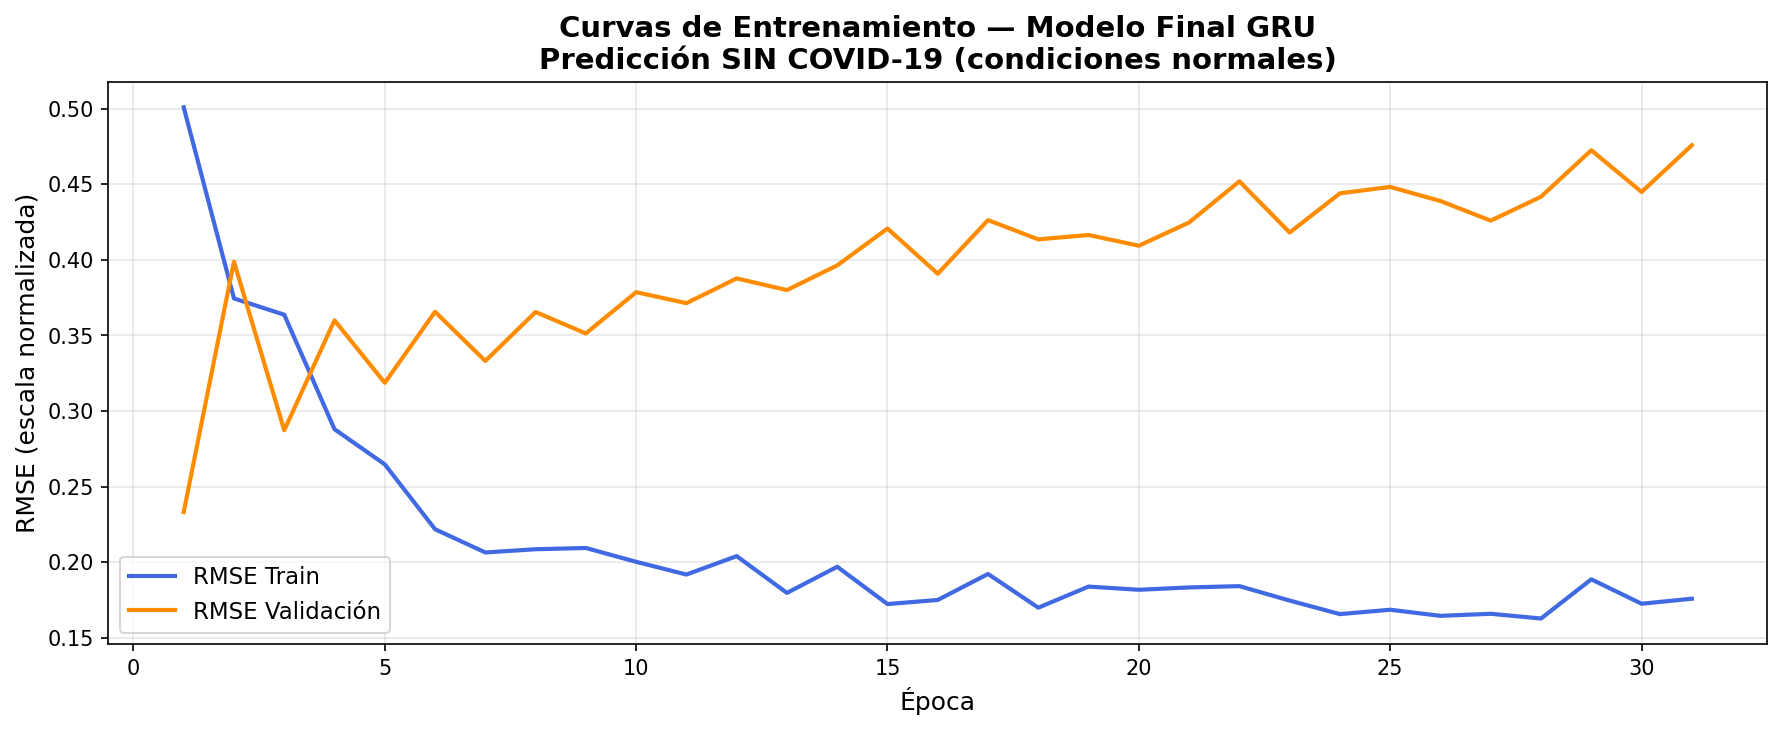
\includegraphics[width=\textwidth]{predicciones/prediccion_cemento_gru/resultados_sin_covid/final_01_curvas_entrenamiento.png}
    \caption{Curvas de aprendizaje del modelo GRU para cemento --- escenario sin pandemia.}
    \label{fig:gru_cemento_curva_sc}
\end{figure}

\paragraph{Métricas de Evaluación}

\begin{table}[htbp]
    \centering
    \caption{Desempeño del modelo GRU para cemento --- escenario sin pandemia: RMSE en train, val y test.}
    \label{tab:gru_cemento_sc_metricas}
    \begin{tabular}{lrrr}
        \toprule
        \textbf{Métrica} & \textbf{Train} & \textbf{Val} & \textbf{Test} \\
        \midrule
        RMSE (Gs.) & 4.911{,}67 & 2.862{,}84 & 2.709{,}13 \\
        \bottomrule
    \end{tabular}
\end{table}

\justify
El RMSE sobre el conjunto de prueba (Gs.~2.709{,}13) es inferior al RMSE de entrenamiento (Gs.~4.911{,}67) y al de validación (Gs.~2.862{,}84), patrón que indica ausencia de sobreajuste. En términos relativos al rango histórico de la serie (Gs.~48.000--76.036), el RMSE de prueba representa aproximadamente el 9,5\,\% del rango, resultado superior al obtenido por el modelo LSTM del mismo material en el mismo escenario (RMSE test: Gs.~1.619,75).

\paragraph{Evaluación sobre el Conjunto de Prueba}

\begin{figure}[htbp]
    \centering
    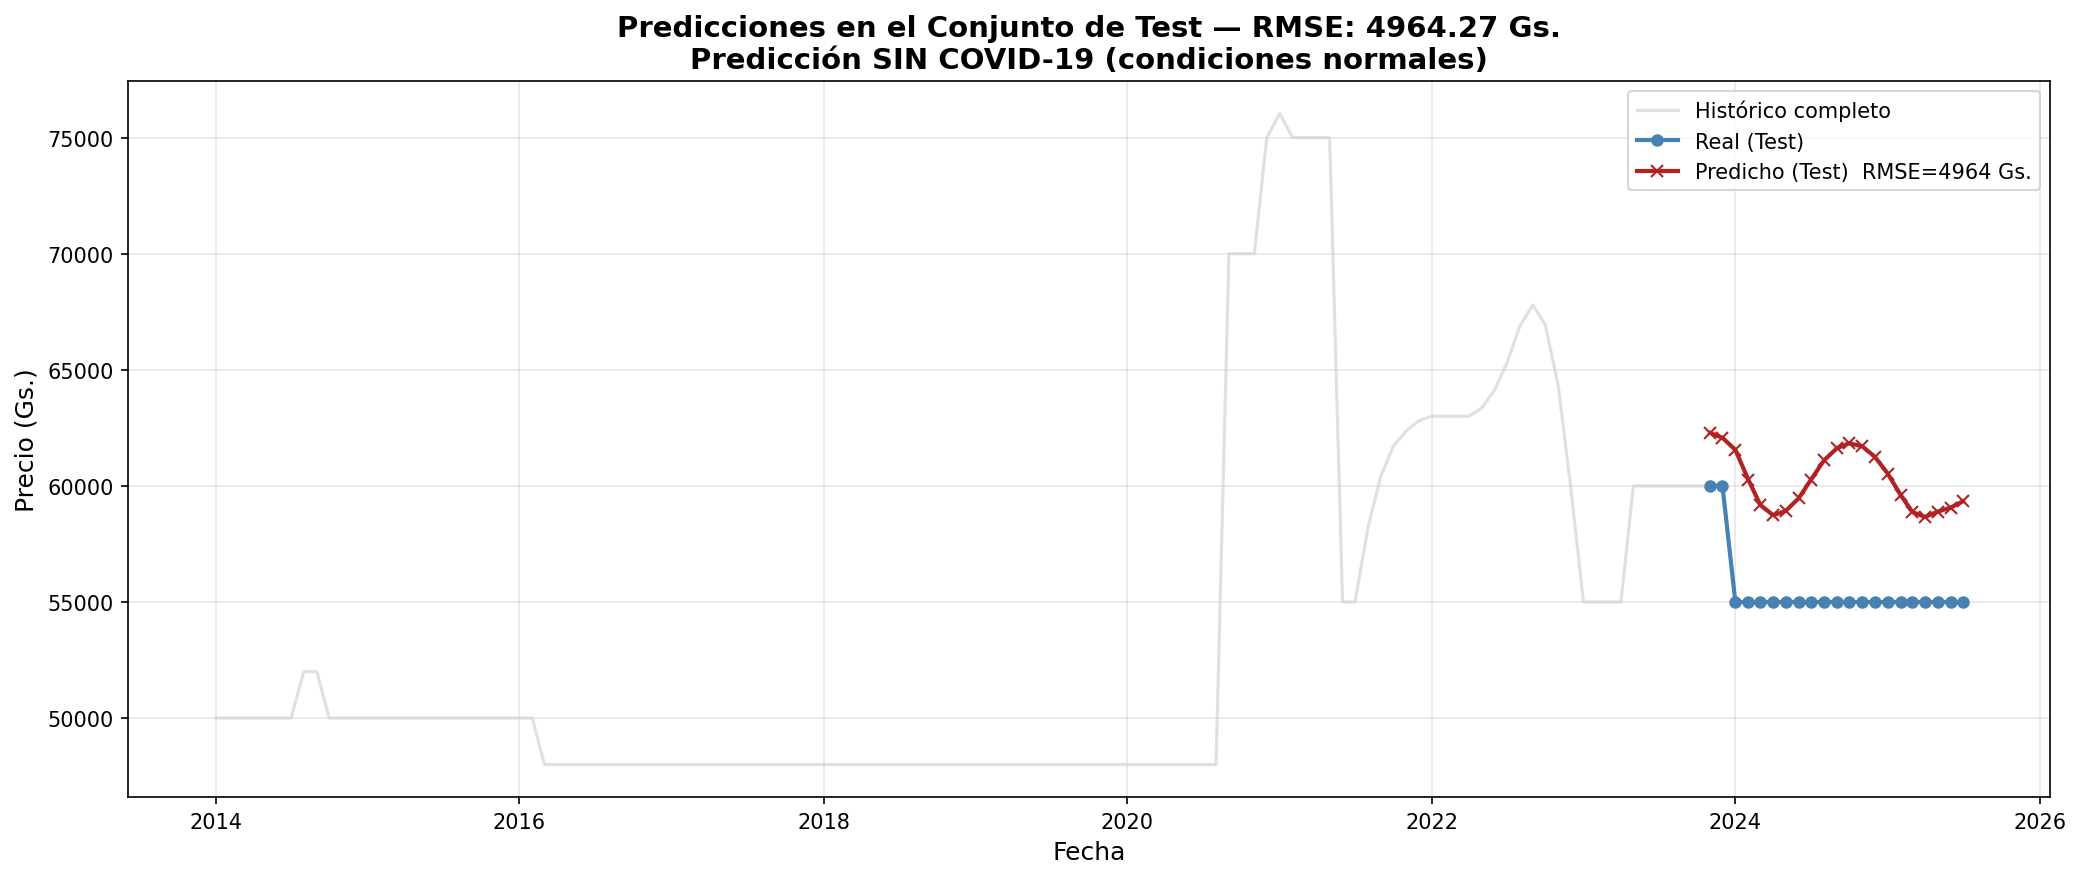
\includegraphics[width=\textwidth]{predicciones/prediccion_cemento_gru/resultados_sin_covid/final_02_prediccion_test_serie.png}
    \caption{Predicción GRU vs.\ valores reales del precio del cemento --- escenario sin pandemia, conjunto de prueba.}
    \label{fig:gru_cemento_test_sc}
\end{figure}

\begin{figure}[htbp]
    \centering
    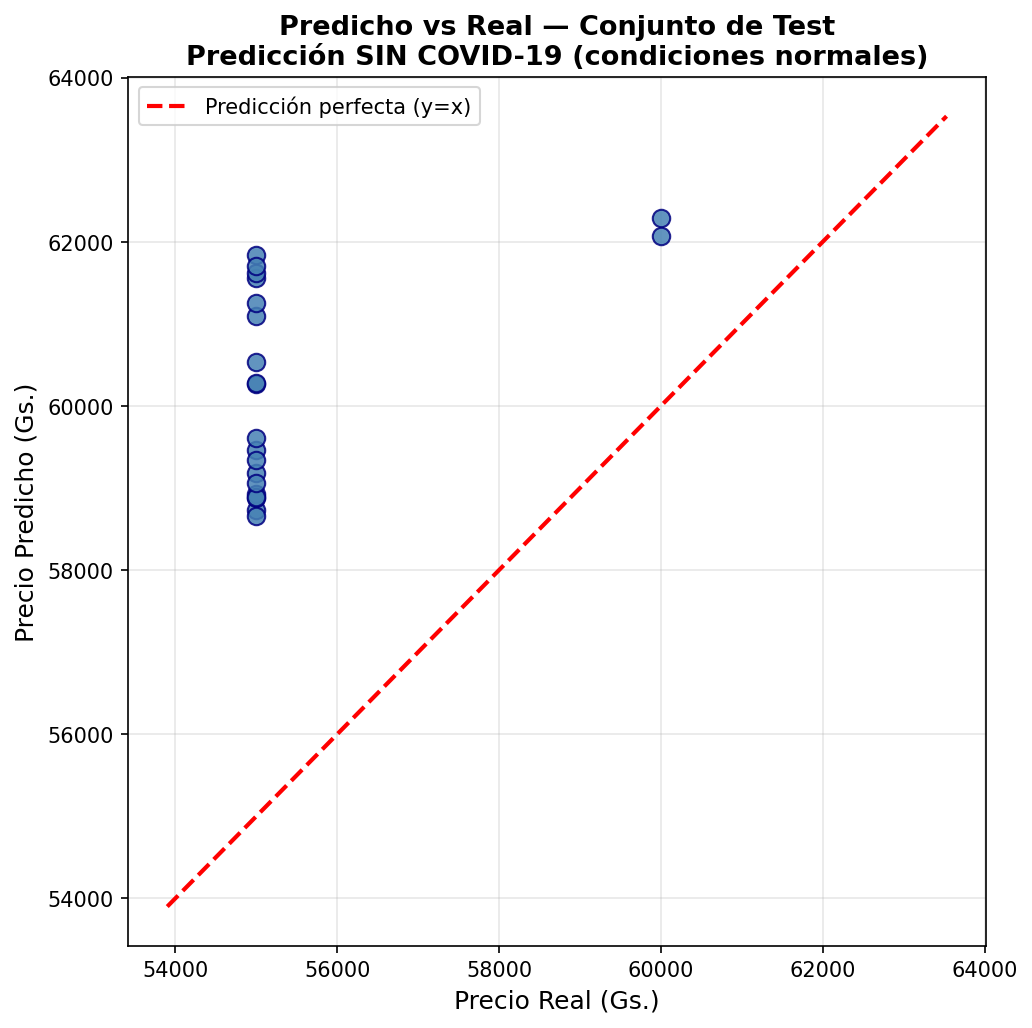
\includegraphics[width=0.8\textwidth]{predicciones/prediccion_cemento_gru/resultados_sin_covid/final_03_scatter_test.png}
    \caption{Diagrama de dispersión: precio predicho vs.\ real del cemento --- escenario sin pandemia (GRU).}
    \label{fig:gru_cemento_scatter_sc}
\end{figure}

\begin{figure}[htbp]
    \centering
    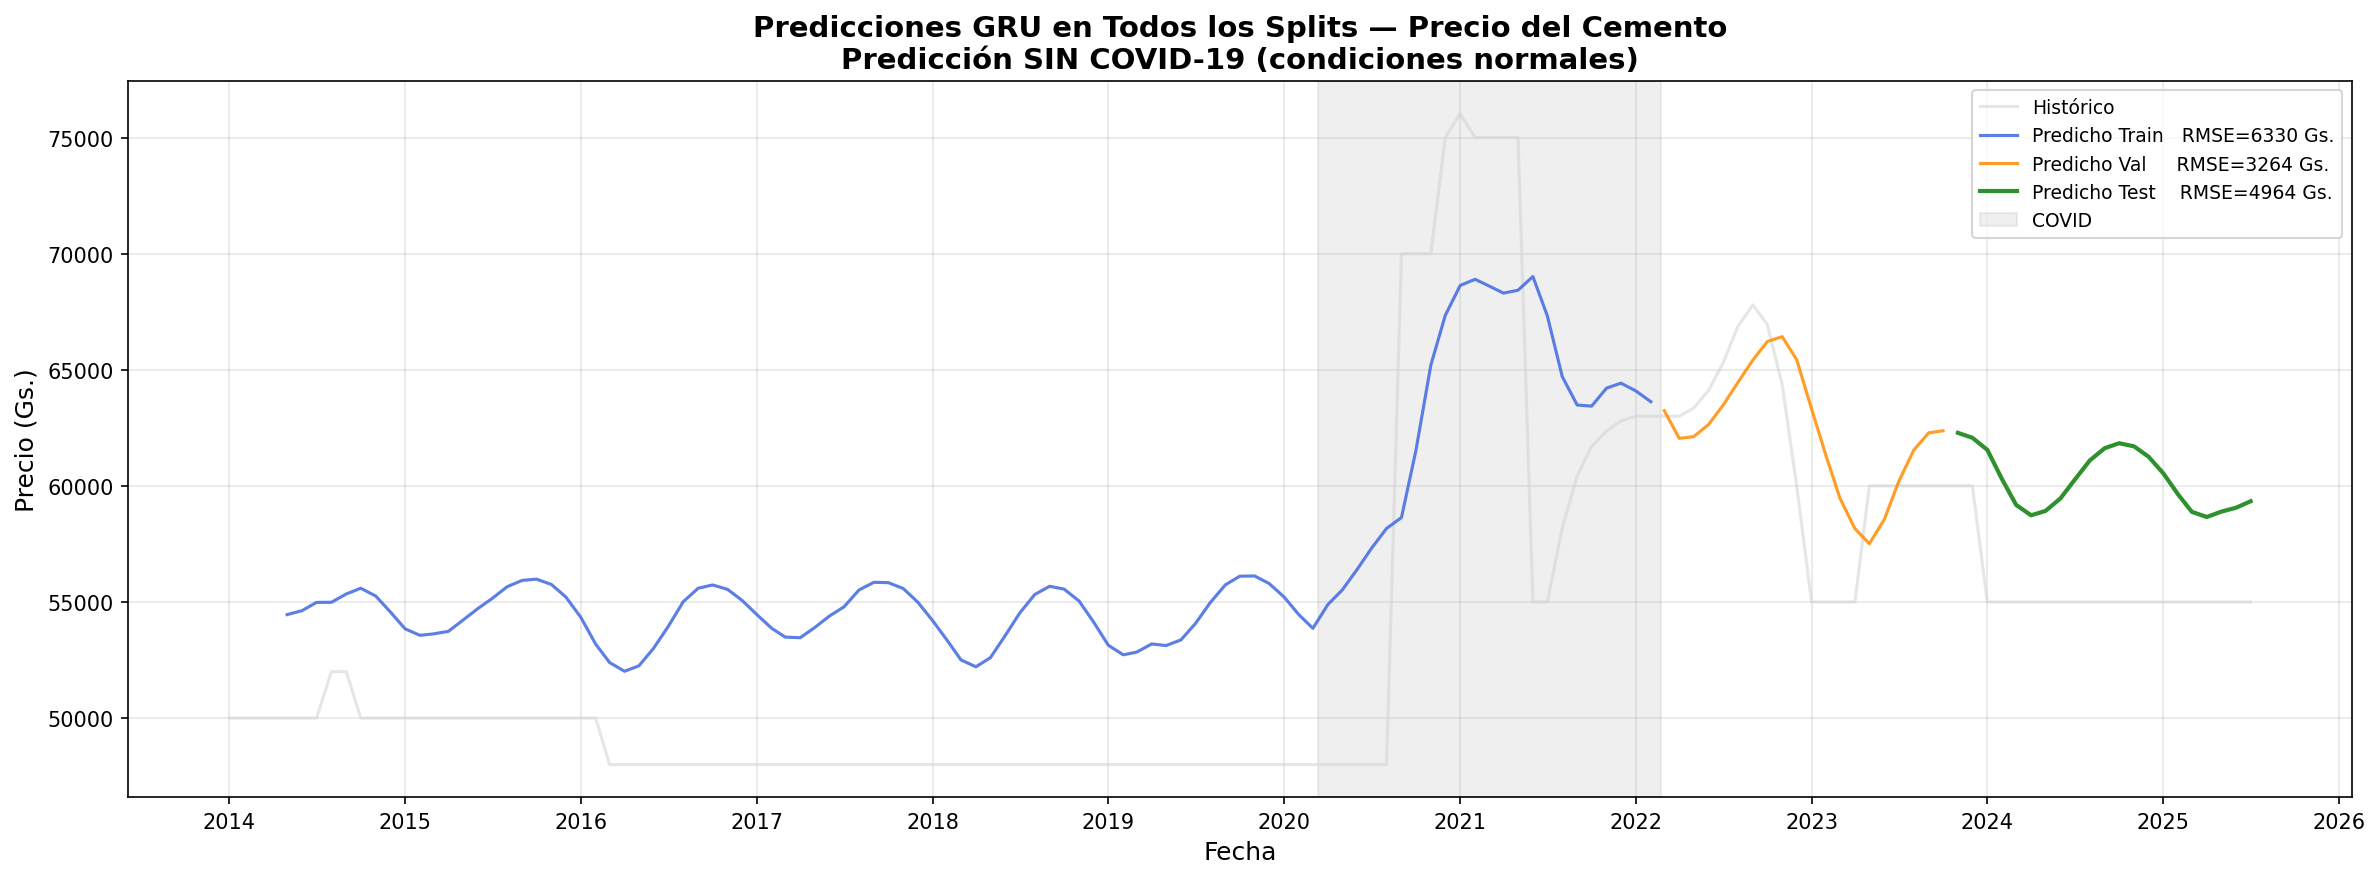
\includegraphics[width=\textwidth]{predicciones/prediccion_cemento_gru/resultados_sin_covid/final_05_todos_splits.png}
    \caption{Ajuste del modelo GRU del cemento sobre las tres particiones --- escenario sin pandemia.}
    \label{fig:gru_cemento_splits_sc}
\end{figure}

\clearpage
\paragraph{Análisis de Residuos}

\begin{figure}[htbp]
    \centering
    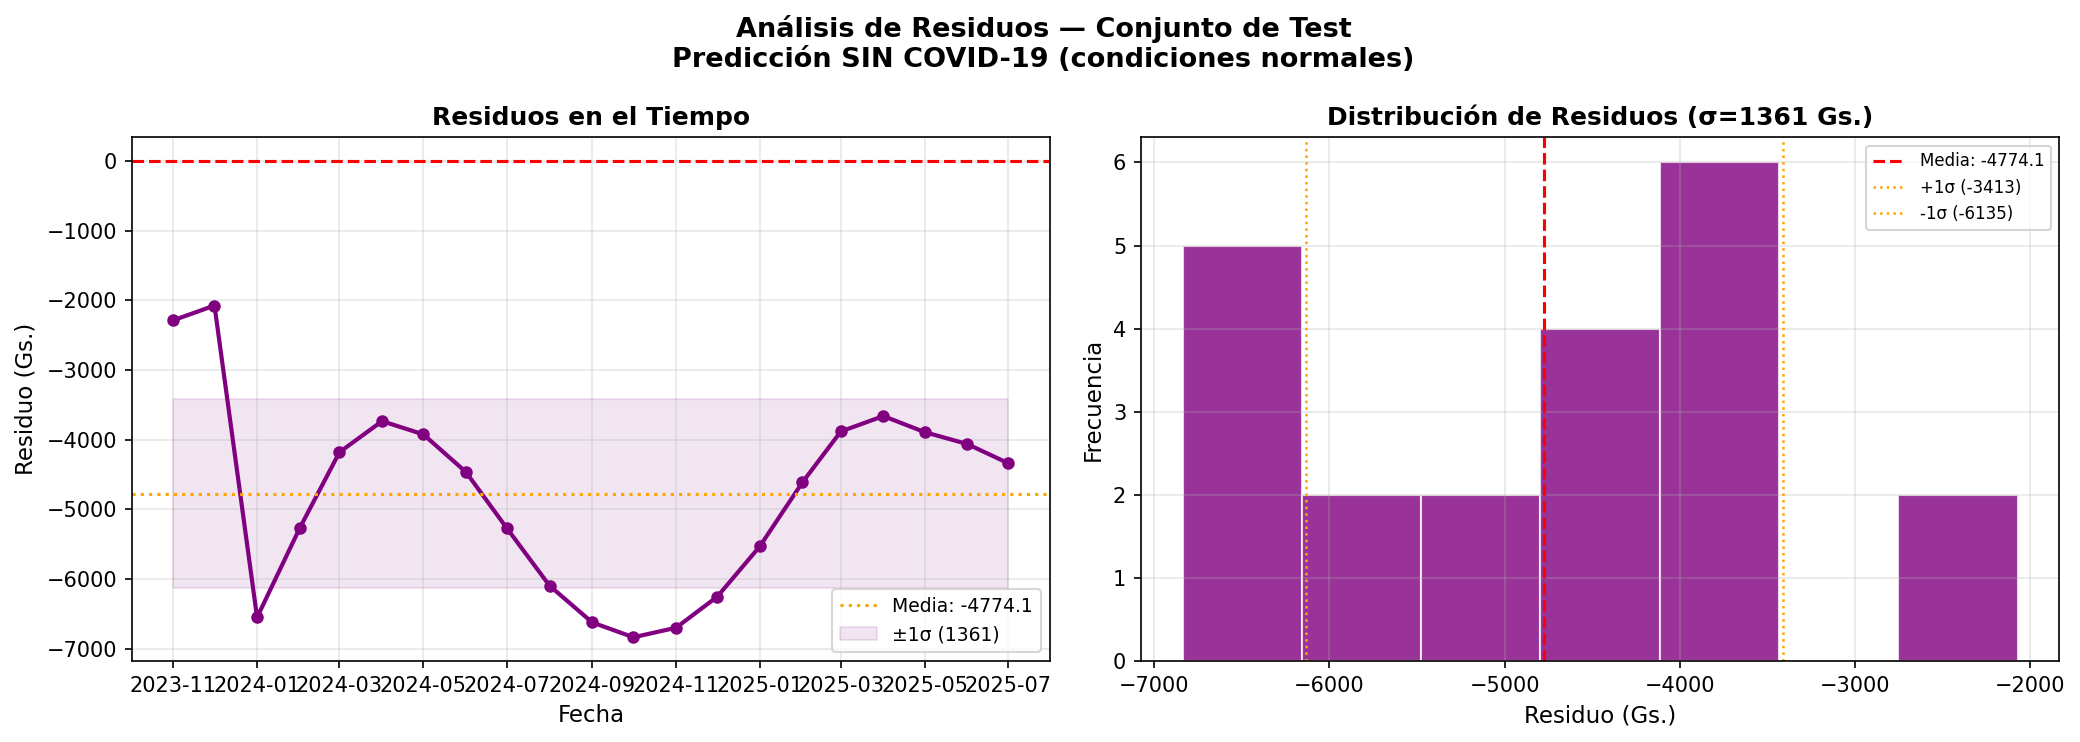
\includegraphics[width=\textwidth]{predicciones/prediccion_cemento_gru/resultados_sin_covid/final_04_residuos.png}
    \caption{Residuos del modelo GRU para cemento --- escenario sin pandemia, conjunto de prueba.}
    \label{fig:gru_cemento_res_sc}
\end{figure}

\begin{figure}[htbp]
    \centering
    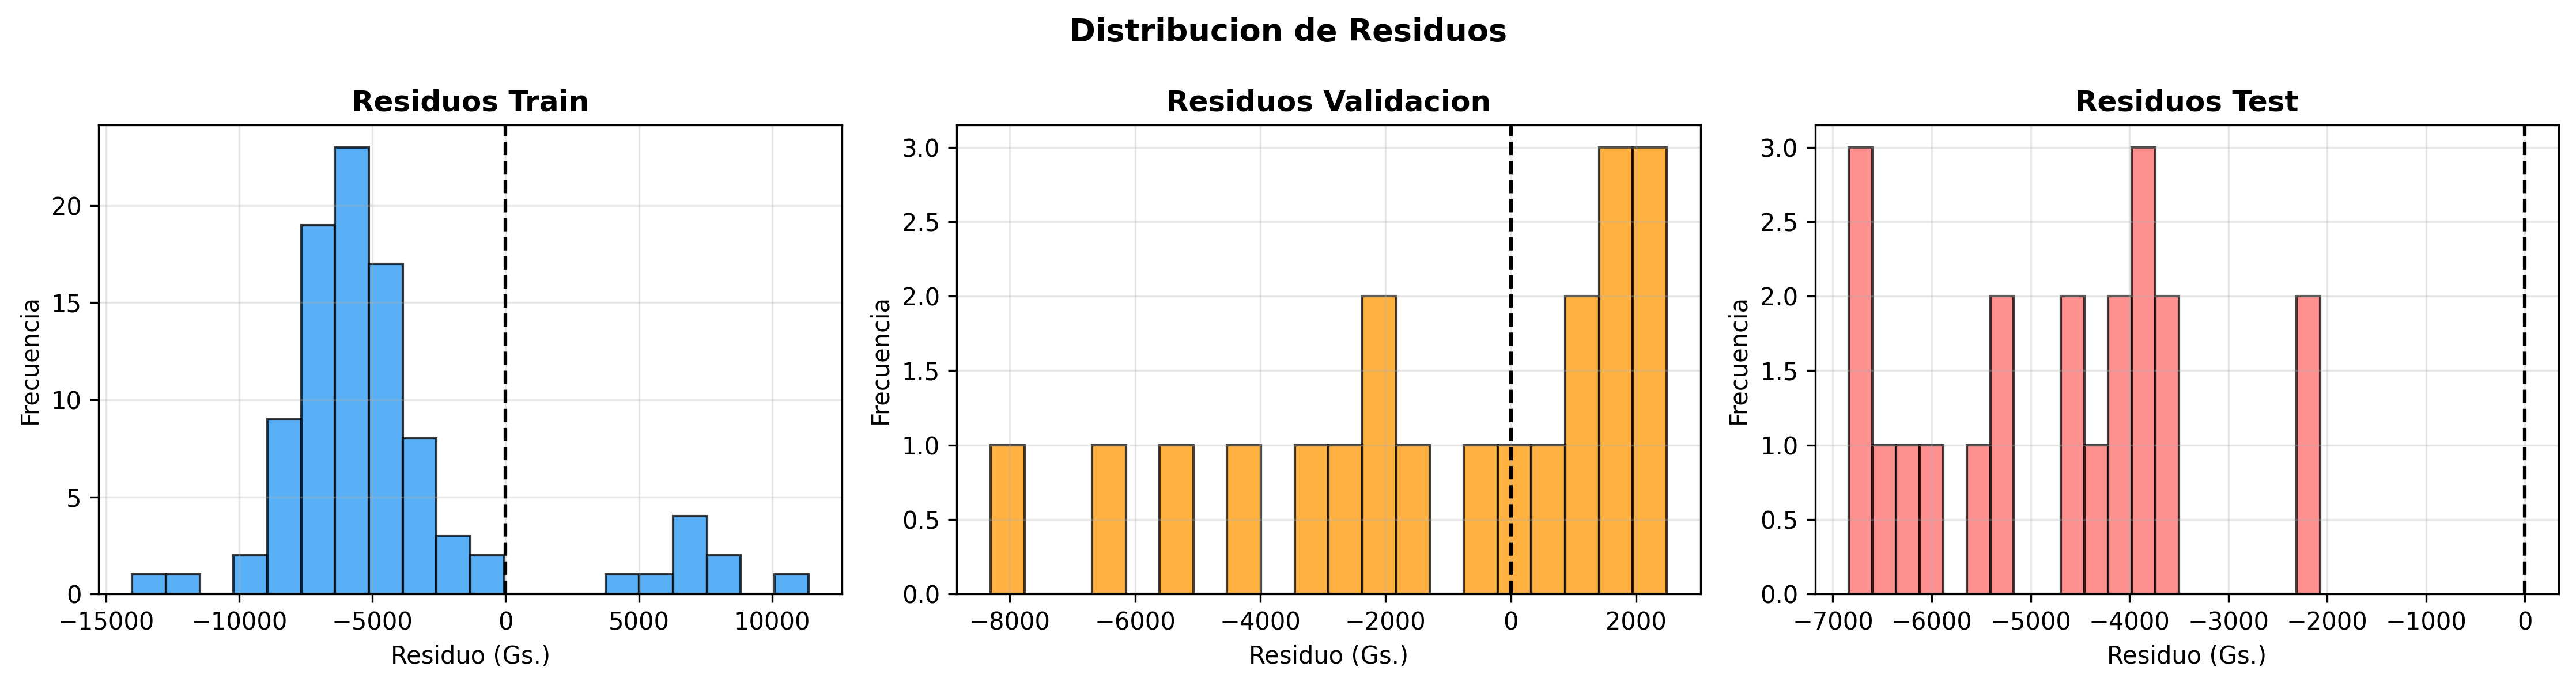
\includegraphics[width=0.8\textwidth]{predicciones/prediccion_cemento_gru/resultados_sin_covid/residuos_histograma.png}
    \caption{Histograma de residuos del modelo GRU para cemento --- escenario sin pandemia.}
    \label{fig:gru_cemento_reshist_sc}
\end{figure}

\begin{figure}[htbp]
    \centering
    \includegraphics[width=\textwidth]{predicciones/prediccion_cemento_gru/resultados_sin_covid/residuos_acf_pacf.png}
    \caption{ACF y PACF de los residuos del modelo GRU para cemento --- escenario sin pandemia.}
    \label{fig:gru_cemento_acf_sc}
\end{figure}

\justify
El test de Ljung-Box sobre los residuos del conjunto de prueba arroja un $p$-valor de 0,002 a 10 rezagos (rechaza $H_0$) y un $p$-valor de 0,077 a 20 rezagos (no rechaza $H_0$). Este resultado intermedio indica que el modelo captura la mayor parte de la estructura temporal, aunque persiste cierta dependencia serial de bajo orden en los primeros rezagos que no logra absorber completamente.

\clearpage
\paragraph{Pronóstico a 24 Meses}

\begin{figure}[htbp]
    \centering
    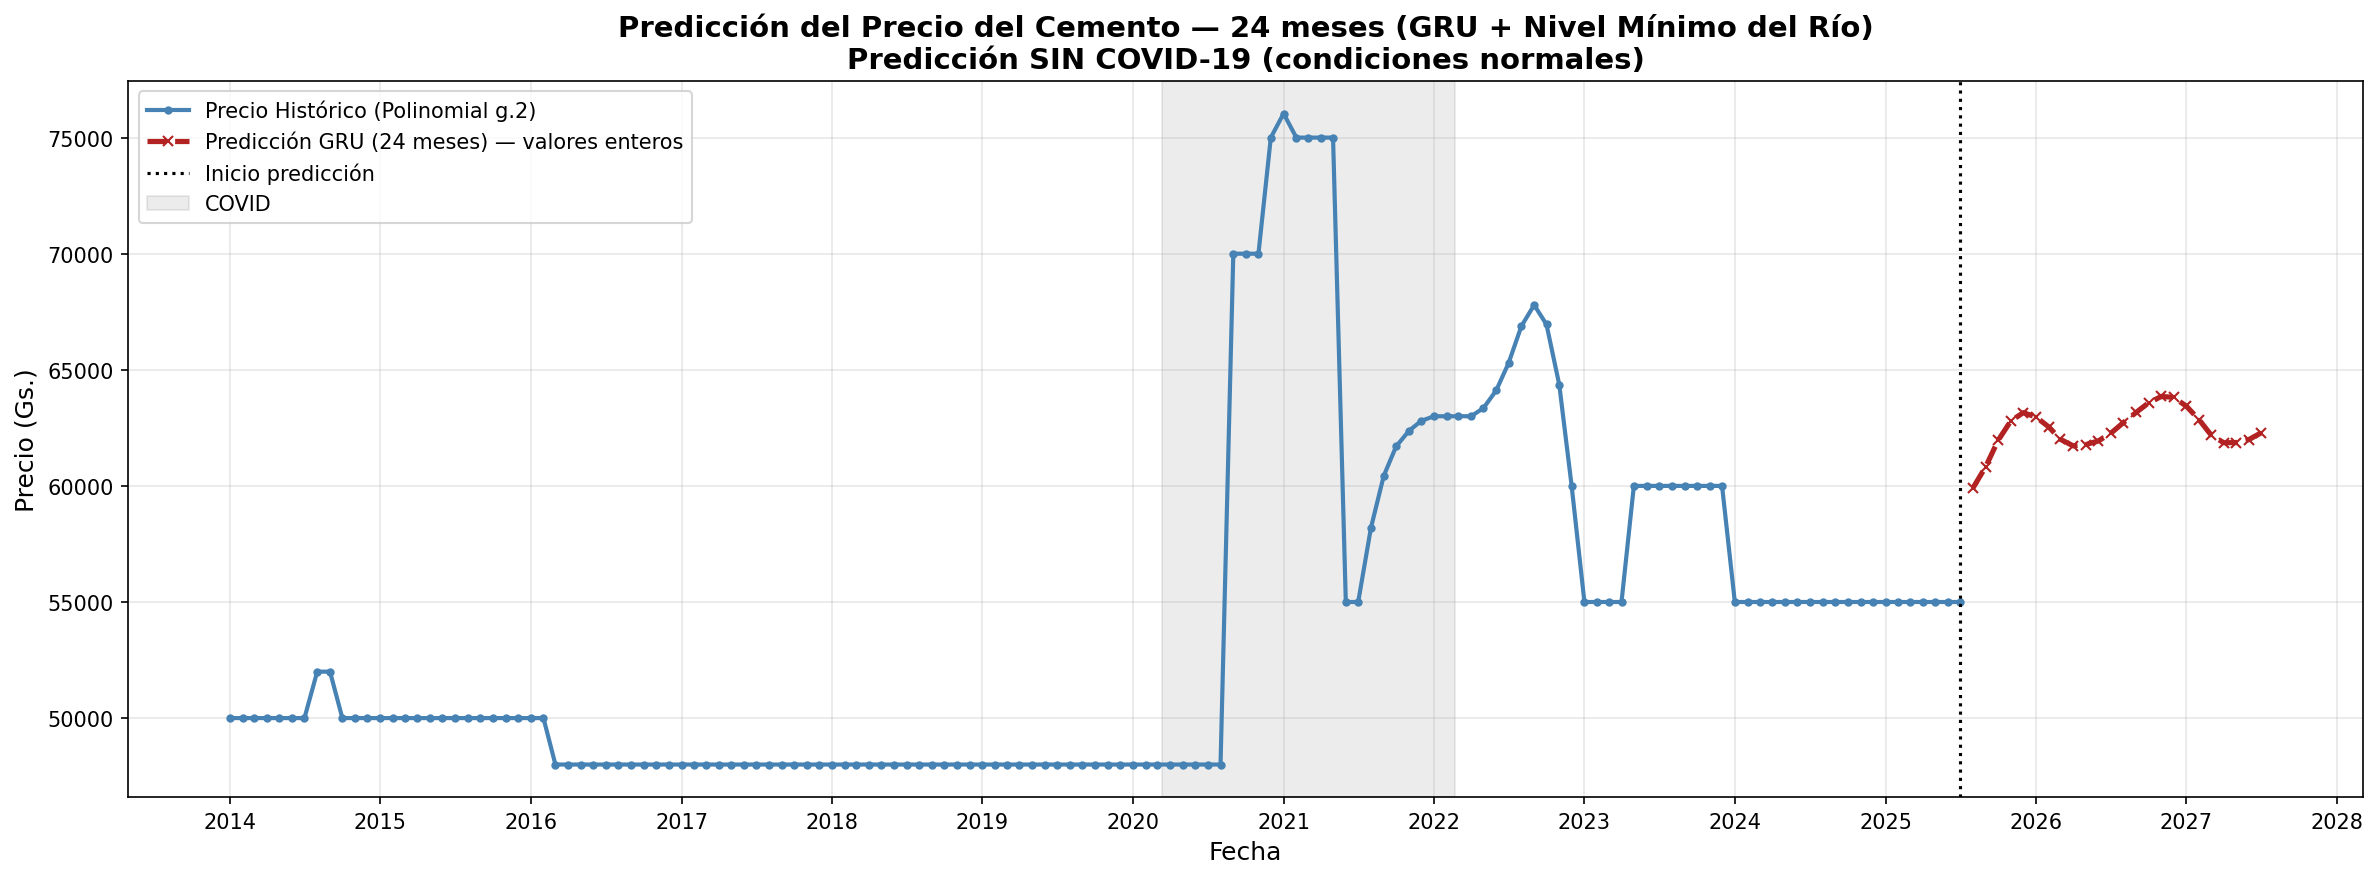
\includegraphics[width=\textwidth]{predicciones/prediccion_cemento_gru/resultados_sin_covid/final_06_prediccion_futura_completa.png}
    \caption{Pronóstico GRU del precio del cemento a 24 meses --- escenario sin pandemia: serie histórica y proyección.}
    \label{fig:gru_cemento_pred_sin_covid}
\end{figure}

\begin{figure}[htbp]
    \centering
    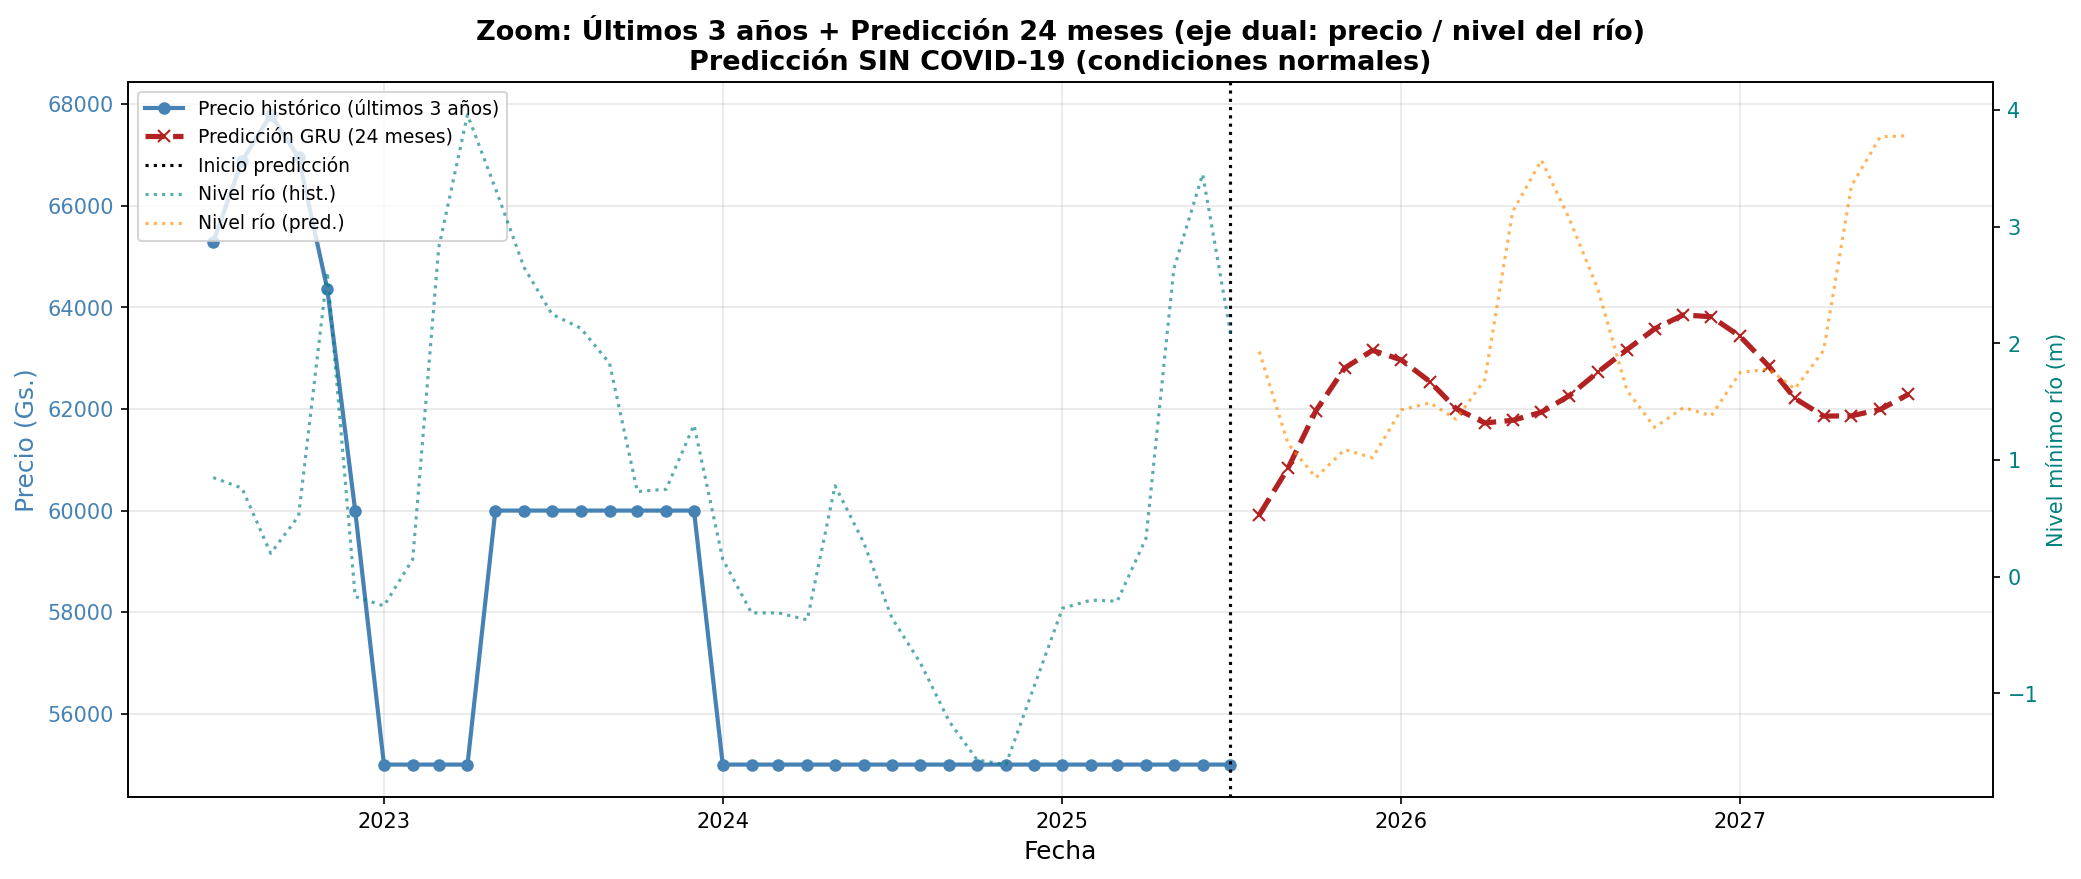
\includegraphics[width=\textwidth]{predicciones/prediccion_cemento_gru/resultados_sin_covid/final_07_prediccion_zoom_dual.png}
    \caption{Zoom sobre la transición entre datos observados y pronóstico GRU del cemento --- escenario sin pandemia.}
    \label{fig:gru_cemento_zoom_sin_covid}
\end{figure}

\begin{figure}[htbp]
    \centering
    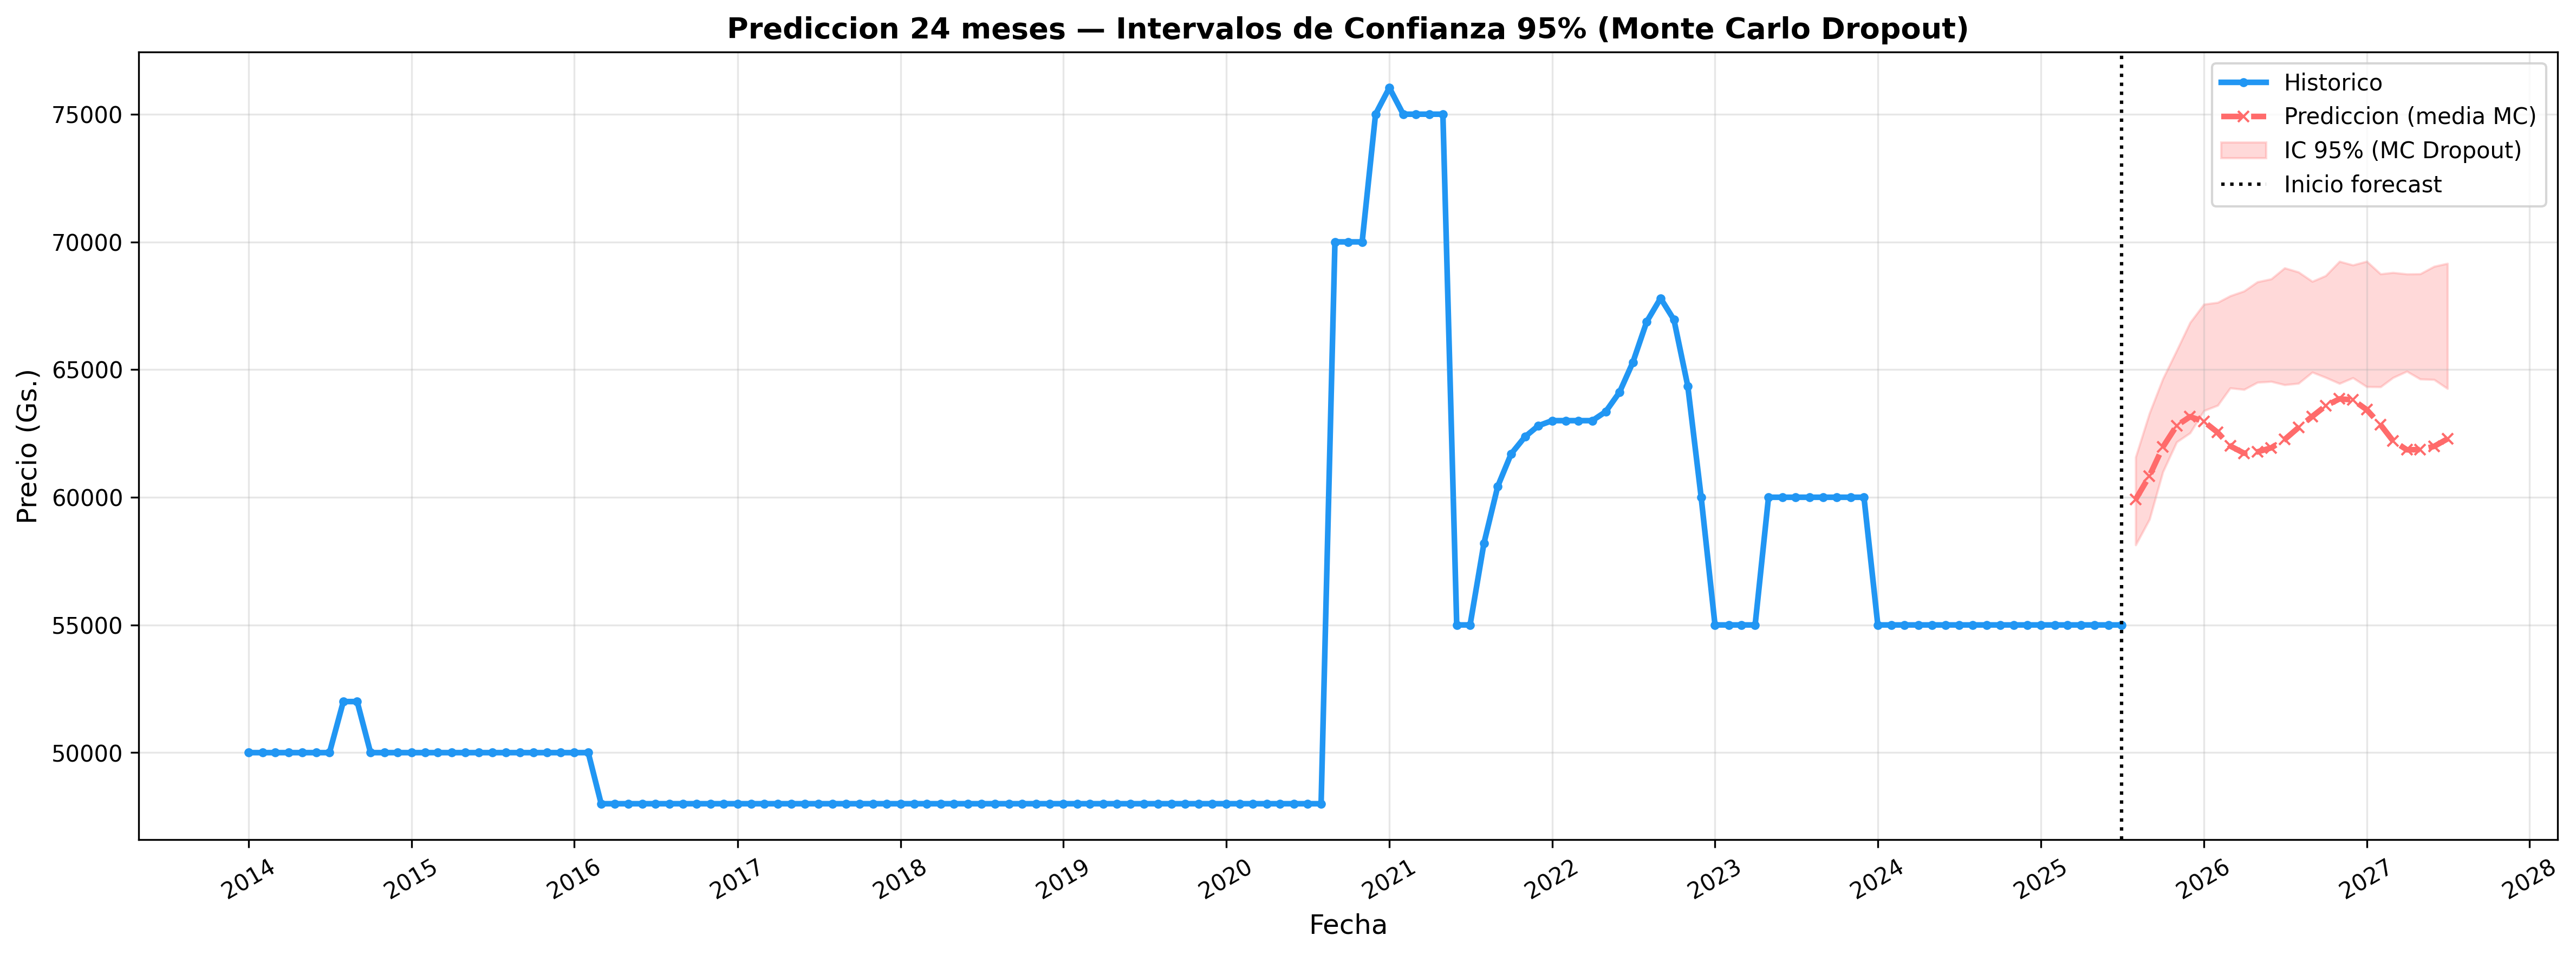
\includegraphics[width=\textwidth]{predicciones/prediccion_cemento_gru/resultados_sin_covid/forecast_ic_monte_carlo.png}
    \caption{IC Monte Carlo Dropout del pronóstico GRU para cemento --- escenario sin pandemia.}
    \label{fig:gru_cemento_ic_sin_covid}
\end{figure}

\justify
El modelo GRU proyecta, bajo el escenario sin pandemia, una tendencia ascendente del precio del cemento durante los primeros meses, alcanzando un máximo de Gs.~61.845 en diciembre de 2025, seguida de un descenso gradual hacia Gs.~55.712 en mayo de 2026 y una leve recuperación posterior. El rango de predicción para todo el horizonte se sitúa entre Gs.~55.600 y Gs.~61.845. La Tabla~\ref{tab:gru_cemento_pred_sc} sintetiza los valores pronosticados para los primeros doce meses.

\begin{table}[htbp]
    \centering
    \caption{Pronóstico GRU del precio del cemento (Gs.) --- escenario sin pandemia, agosto 2025 -- julio 2026.}
    \label{tab:gru_cemento_pred_sc}
    \begin{tabular}{lr}
        \toprule
        \textbf{Mes} & \textbf{Precio Predicho (Gs.)} \\
        \midrule
        Agosto 2025      & 57.693 \\
        Septiembre 2025  & 59.720 \\
        Octubre 2025     & 61.126 \\
        Noviembre 2025   & 61.824 \\
        Diciembre 2025   & 61.845 \\
        Enero 2026       & 61.009 \\
        Febrero 2026     & 59.763 \\
        Marzo 2026       & 58.206 \\
        Abril 2026       & 56.642 \\
        Mayo 2026        & 55.712 \\
        Junio 2026       & 56.018 \\
        Julio 2026       & 56.846 \\
        \bottomrule
    \end{tabular}
\end{table}

% ------ CEMENTO GRU CON COVID ------
\clearpage
\subsubsection{Escenario con Efecto Pandémico}

\paragraph{Hiperparámetros y Arquitectura}

\justify
Para el escenario con efecto pandémico, la búsqueda con Optuna convergió a una configuración diferente: una capa GRU unidireccional con 64 unidades ocultas, sin \textit{dropout} ni planificador de tasa de aprendizaje. El optimizador fue Adam con $\eta = 0{,}001$ y regularización L2 $\lambda=10^{-5}$, \textit{lookback} de 6 meses y \textit{batch size} de 4. La arquitectura resultante totaliza los mismos 14.081 parámetros entrenables, pero con una dinámica de entrenamiento más simple. La Tabla~\ref{tab:gru_cemento_cc_arq} resume estos parámetros.

\begin{table}[htbp]
    \centering
    \caption{Hiperparámetros del modelo GRU para cemento --- escenario con pandemia.}
    \label{tab:gru_cemento_cc_arq}
    \begin{tabular}{ll}
        \toprule
        \textbf{Hiperparámetro} & \textbf{Valor} \\
        \midrule
        Capas GRU              & 1 (unidireccional) \\
        Unidades ocultas       & 64 \\
        Lookback               & 6 meses \\
        Optimizador            & Adam ($\eta=0{,}001$, WD $=10^{-5}$) \\
        Batch size             & 4 \\
        Dropout / Rec.\ dropout & 0{,}0 / 0{,}0 \\
        Scheduler              & Ninguno \\
        Parámetros entrenables & 14.081 \\
        \bottomrule
    \end{tabular}
\end{table}

\paragraph{Curva de Aprendizaje}

\begin{figure}[htbp]
    \centering
    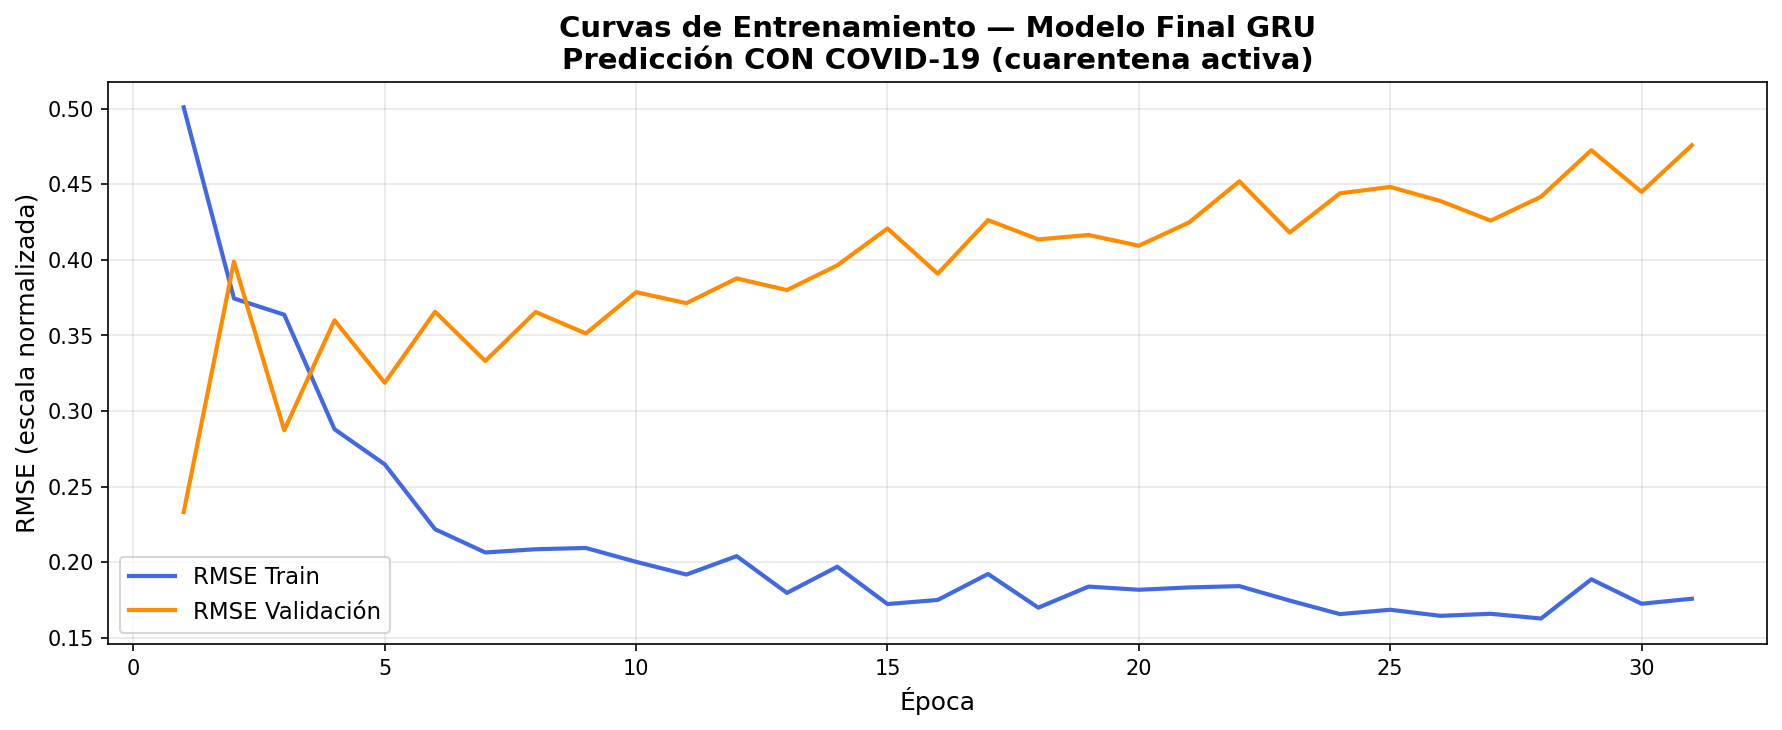
\includegraphics[width=\textwidth]{predicciones/prediccion_cemento_gru/resultados_con_covid/final_01_curvas_entrenamiento.png}
    \caption{Curvas de aprendizaje del modelo GRU para cemento --- escenario con pandemia.}
    \label{fig:gru_cemento_curva_cc}
\end{figure}

\paragraph{Métricas de Evaluación}

\begin{table}[htbp]
    \centering
    \caption{Desempeño del modelo GRU para cemento --- escenario con pandemia: RMSE en train, val y test.}
    \label{tab:gru_cemento_cc_metricas}
    \begin{tabular}{lrrr}
        \toprule
        \textbf{Métrica} & \textbf{Train} & \textbf{Val} & \textbf{Test} \\
        \midrule
        RMSE (Gs.) & 5.343{,}63 & 4.130{,}82 & 1.694{,}23 \\
        \bottomrule
    \end{tabular}
\end{table}

\justify
El RMSE de prueba para el escenario con pandemia (Gs.~1.694{,}23) resulta notablemente inferior al obtenido en el escenario sin pandemia (Gs.~2.709{,}13), lo que indica que la inclusión de la variable pandémica en el entrenamiento mejora el ajuste del modelo sobre el período de evaluación. Sin embargo, el RMSE de entrenamiento (Gs.~5.343{,}63) es más elevado que en el escenario sin pandemia (Gs.~4.911{,}67), lo que puede atribuirse a la mayor variabilidad introducida por los datos pandémicos en el conjunto de entrenamiento.

\paragraph{Evaluación sobre el Conjunto de Prueba}

\begin{figure}[htbp]
    \centering
    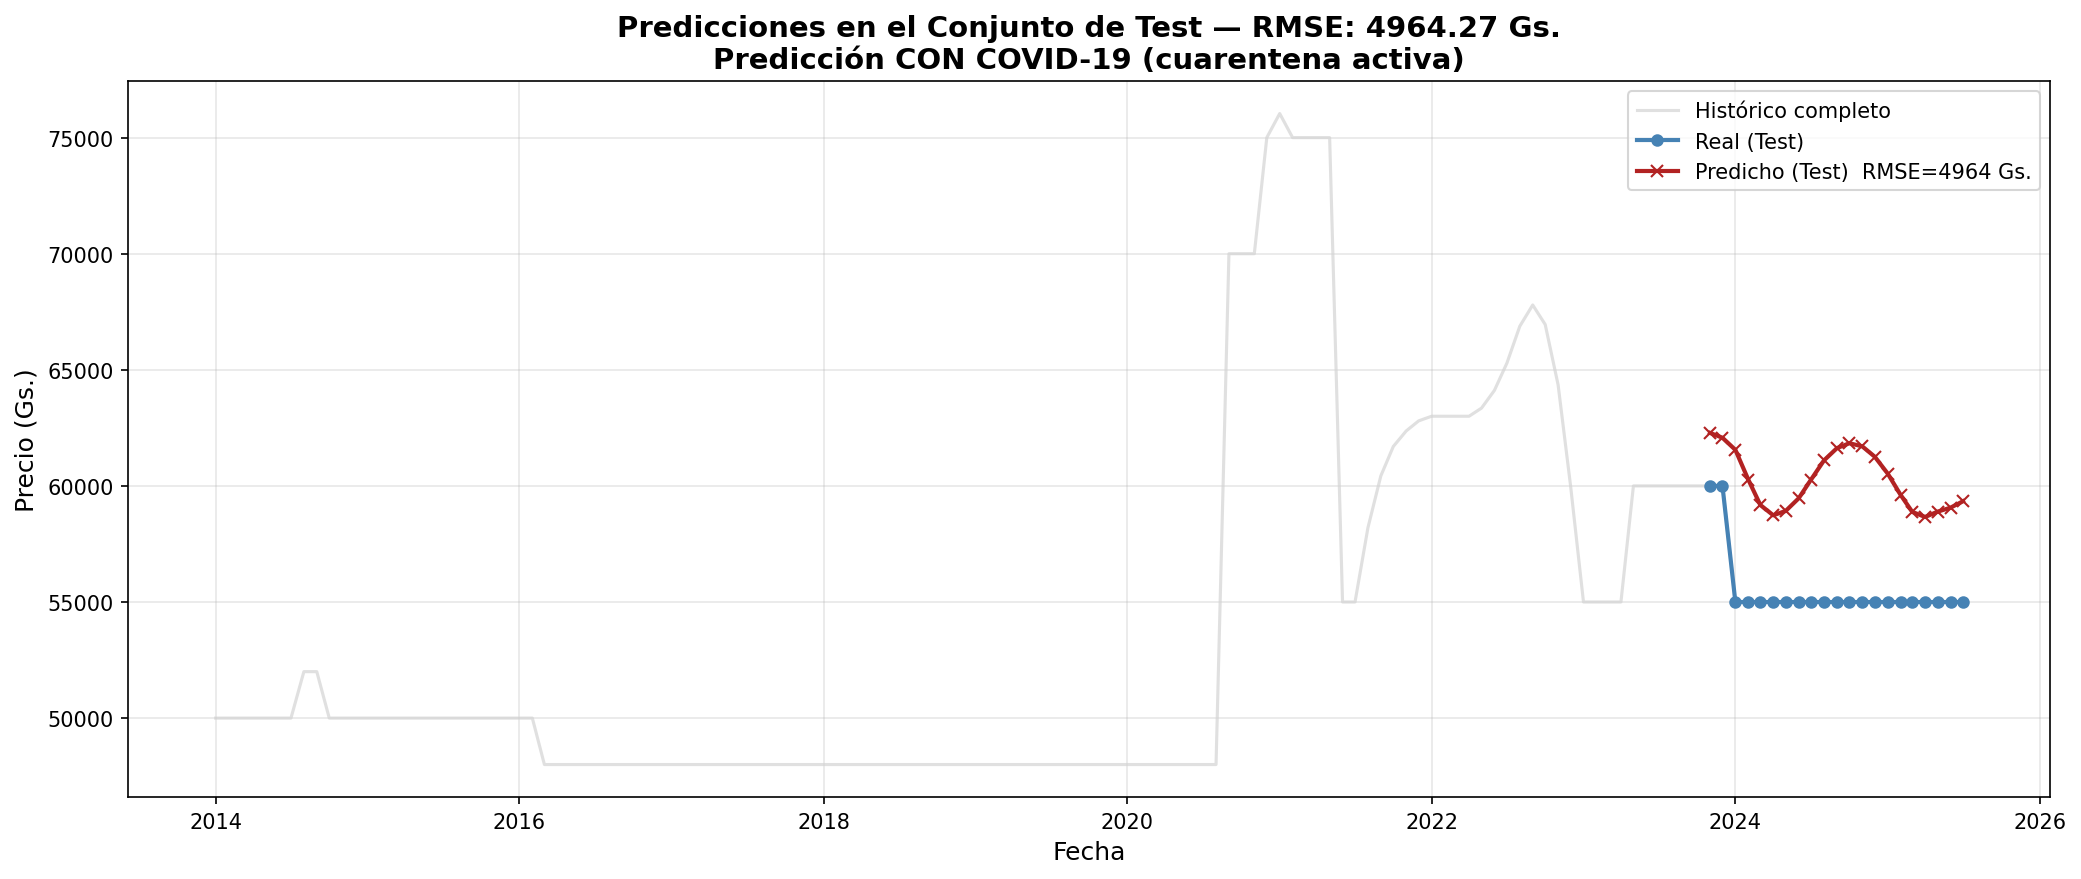
\includegraphics[width=\textwidth]{predicciones/prediccion_cemento_gru/resultados_con_covid/final_02_prediccion_test_serie.png}
    \caption{Predicción GRU vs.\ valores reales del precio del cemento --- escenario con pandemia, conjunto de prueba.}
    \label{fig:gru_cemento_test_cc}
\end{figure}

\begin{figure}[htbp]
    \centering
    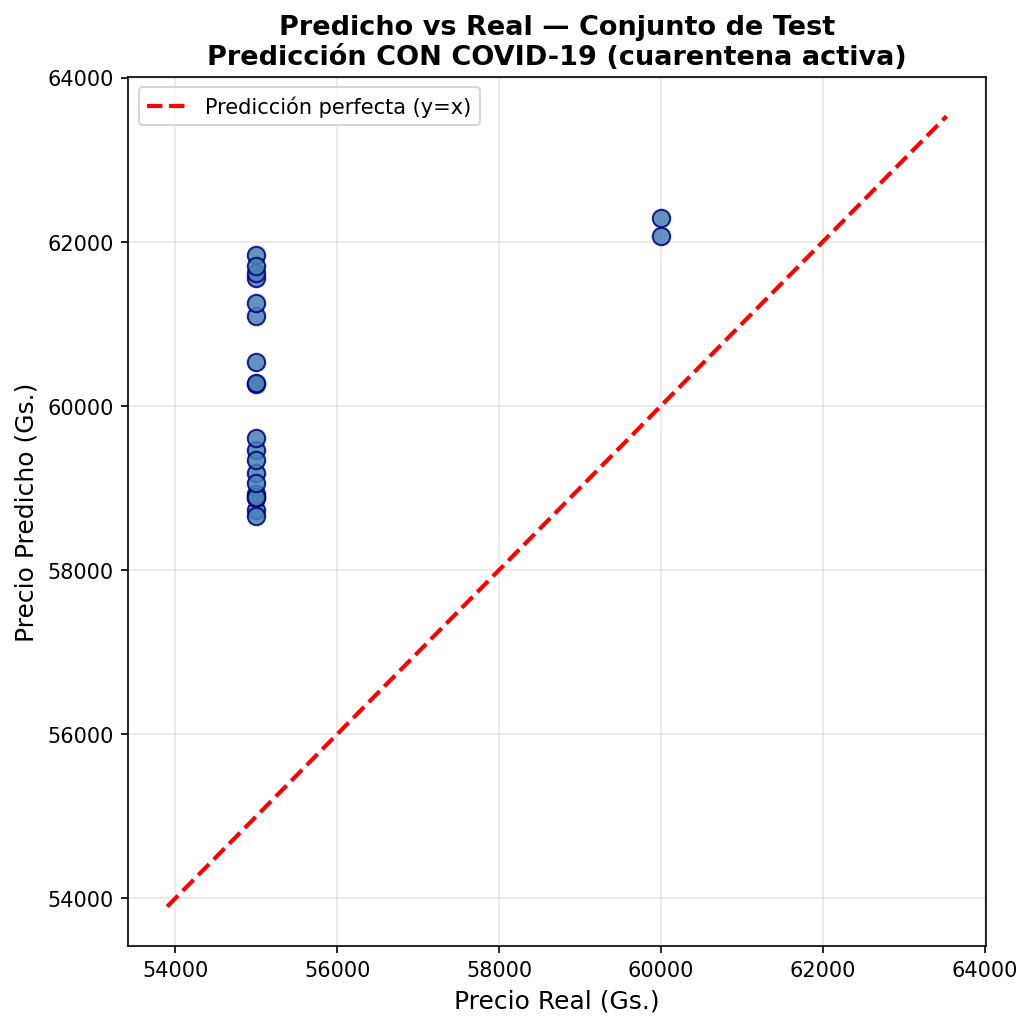
\includegraphics[width=0.8\textwidth]{predicciones/prediccion_cemento_gru/resultados_con_covid/final_03_scatter_test.png}
    \caption{Diagrama de dispersión: precio predicho vs.\ real del cemento --- escenario con pandemia (GRU).}
    \label{fig:gru_cemento_scatter_cc}
\end{figure}

\begin{figure}[htbp]
    \centering
    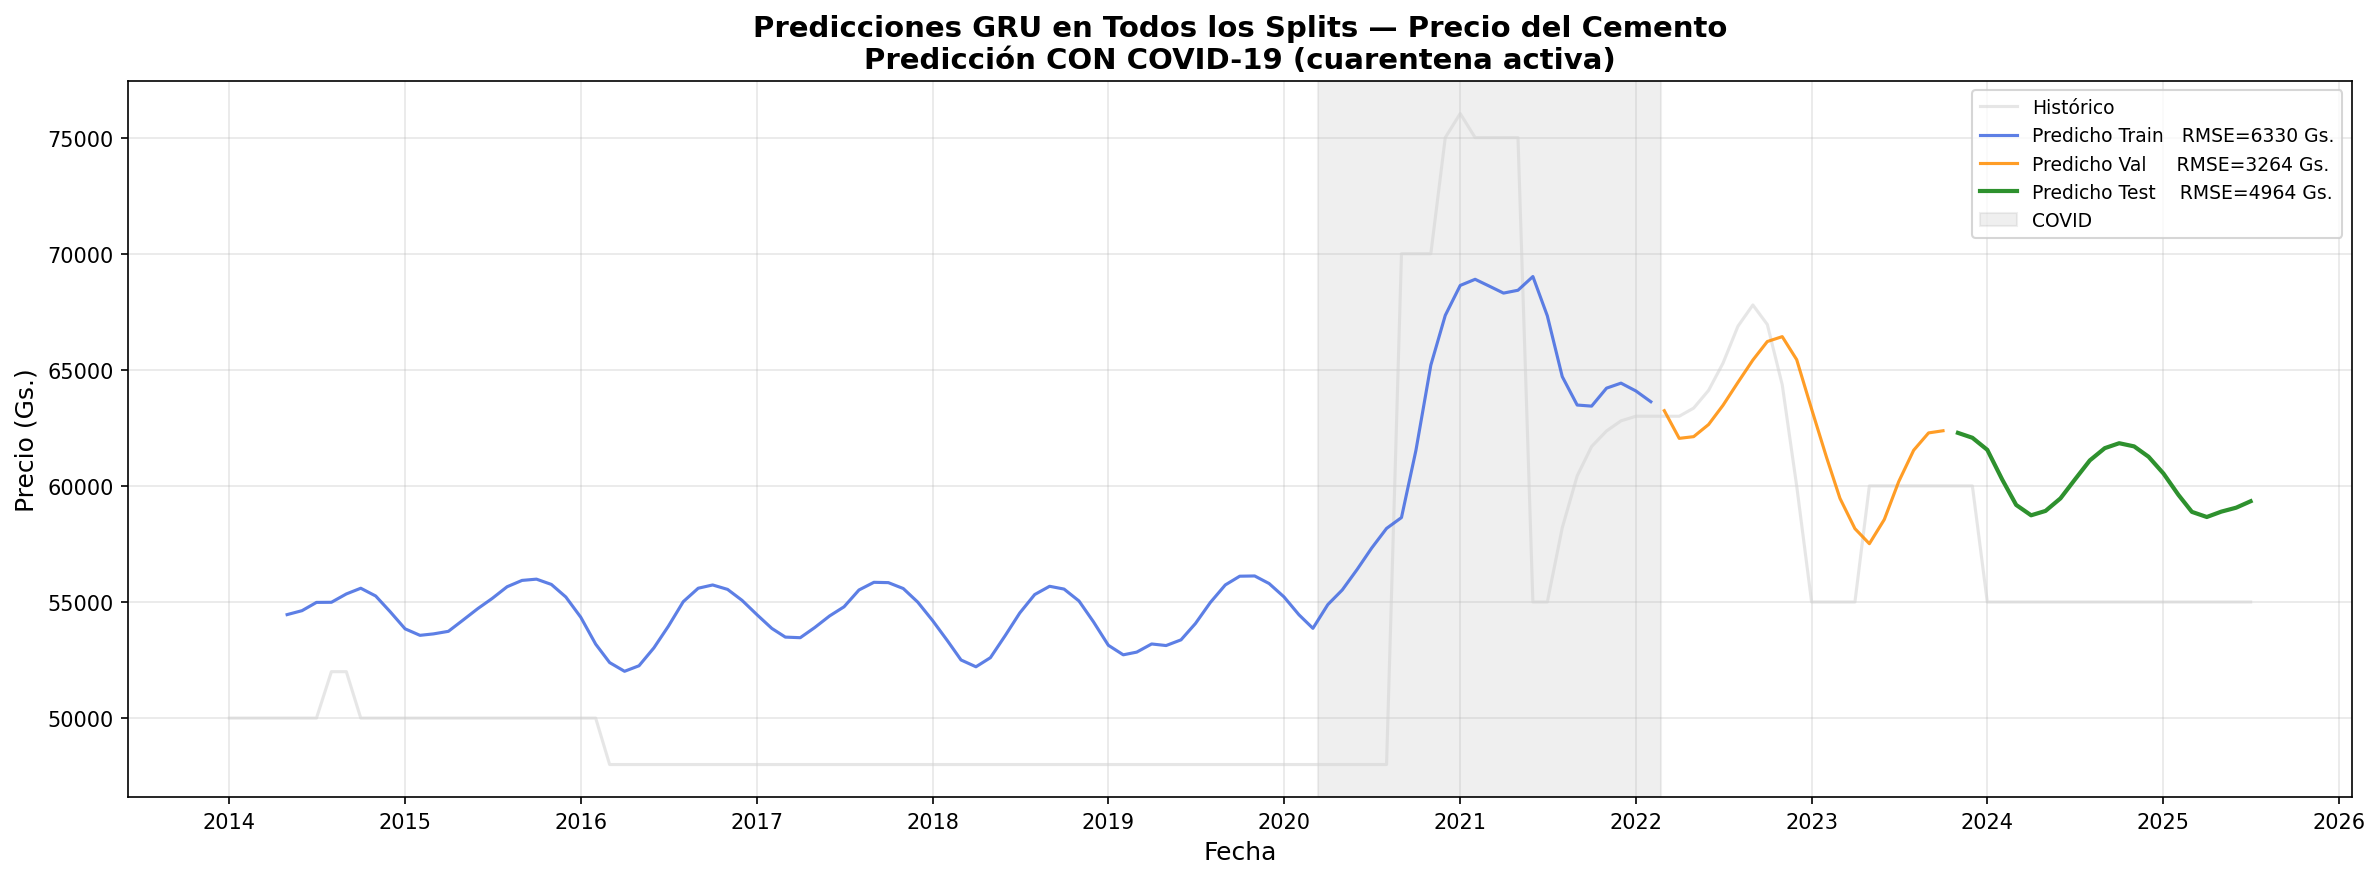
\includegraphics[width=\textwidth]{predicciones/prediccion_cemento_gru/resultados_con_covid/final_05_todos_splits.png}
    \caption{Ajuste del modelo GRU del cemento sobre las tres particiones --- escenario con pandemia.}
    \label{fig:gru_cemento_splits_cc}
\end{figure}

\clearpage
\paragraph{Análisis de Residuos}

\begin{figure}[htbp]
    \centering
    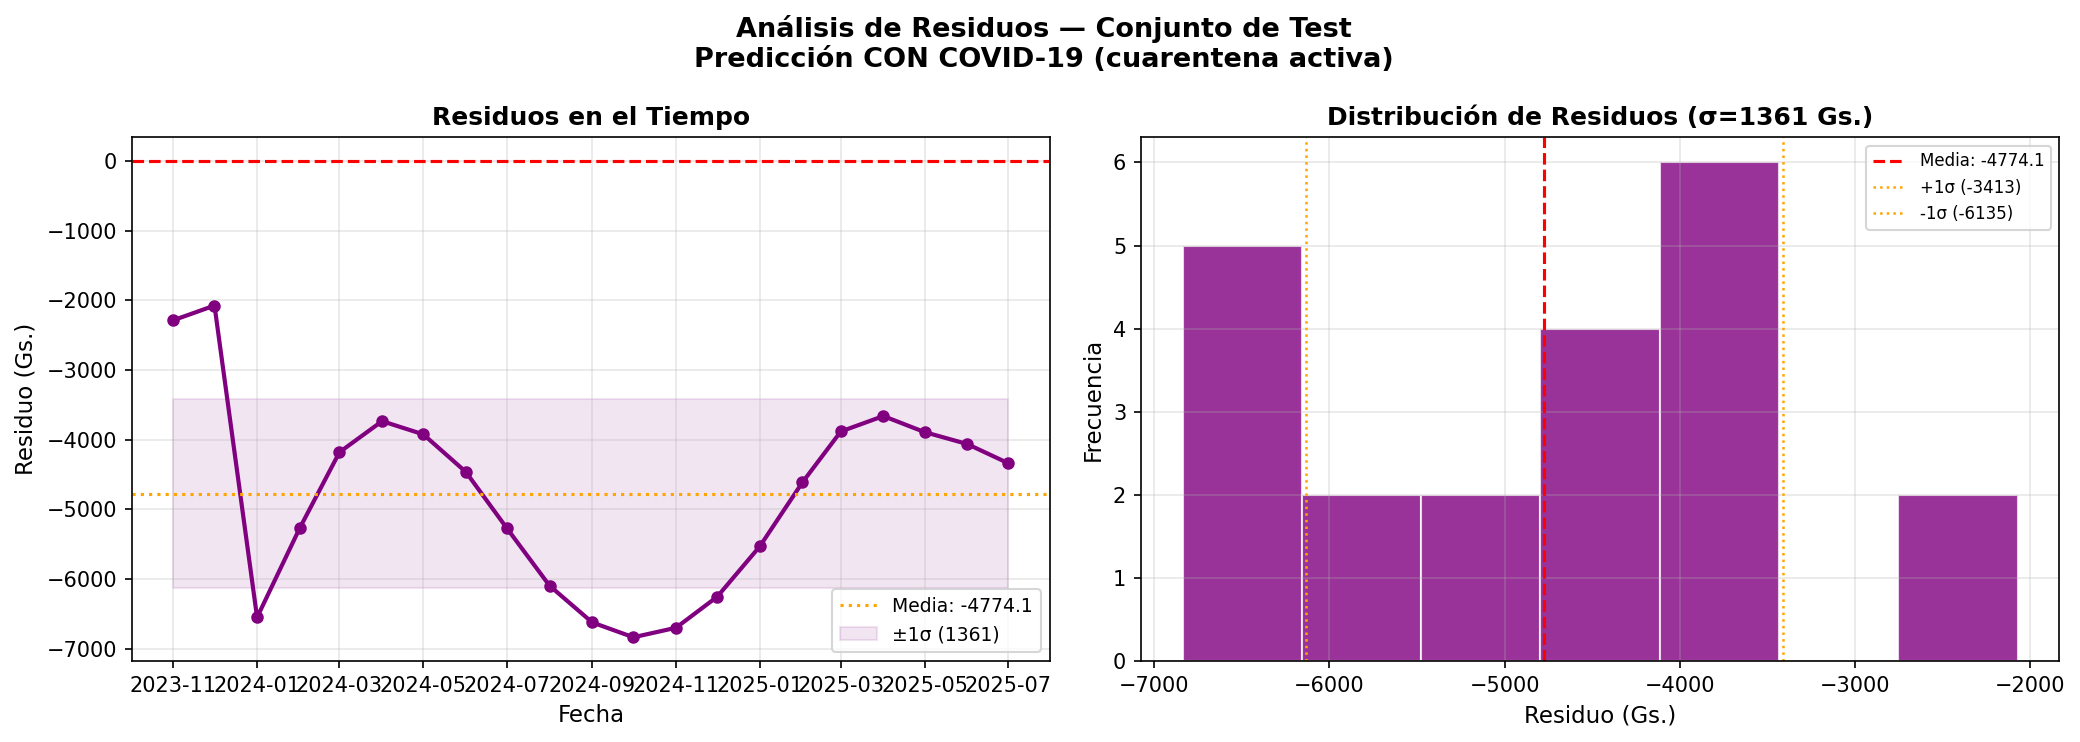
\includegraphics[width=\textwidth]{predicciones/prediccion_cemento_gru/resultados_con_covid/final_04_residuos.png}
    \caption{Residuos del modelo GRU para cemento --- escenario con pandemia, conjunto de prueba.}
    \label{fig:gru_cemento_res_cc}
\end{figure}

\begin{figure}[htbp]
    \centering
    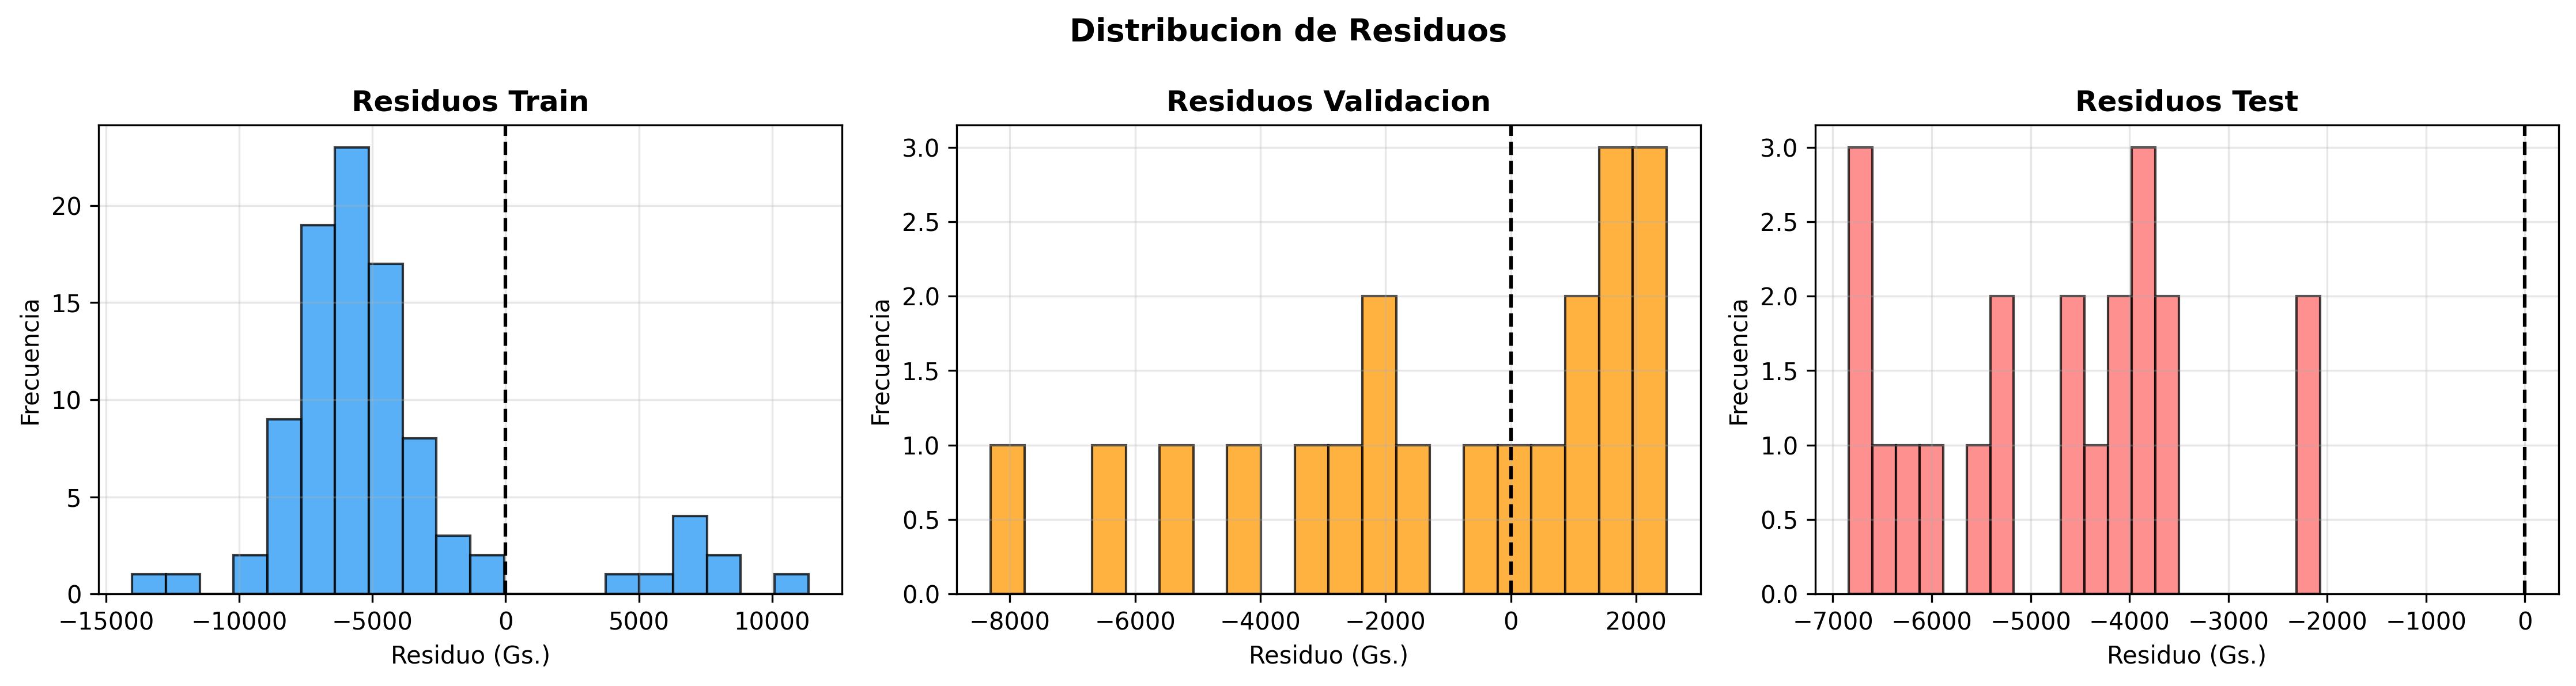
\includegraphics[width=0.8\textwidth]{predicciones/prediccion_cemento_gru/resultados_con_covid/residuos_histograma.png}
    \caption{Histograma de residuos del modelo GRU para cemento --- escenario con pandemia.}
    \label{fig:gru_cemento_reshist_cc}
\end{figure}

\begin{figure}[htbp]
    \centering
    \includegraphics[width=\textwidth]{predicciones/prediccion_cemento_gru/resultados_con_covid/residuos_acf_pacf.png}
    \caption{ACF y PACF de los residuos del modelo GRU para cemento --- escenario con pandemia.}
    \label{fig:gru_cemento_acf_cc}
\end{figure}

\justify
El test de Ljung-Box sobre los residuos del conjunto de prueba arroja un $p$-valor de 0,080 a 10 rezagos y de 0,151 a 20 rezagos, ambos superiores al umbral de 0,05. Esto confirma que los residuos del modelo GRU del cemento bajo el escenario con pandemia se comportan como ruido blanco, resultado más favorable que el obtenido en el escenario sin pandemia (donde existía autocorrelación a 10 rezagos). La inclusión de la variable pandémica parece haber reducido la autocorrelación residual, posiblemente al absorber parte de la estructura temporal que el modelo sin ese indicador no podía explicar.

\clearpage
\paragraph{Pronóstico a 24 Meses}

\begin{figure}[htbp]
    \centering
    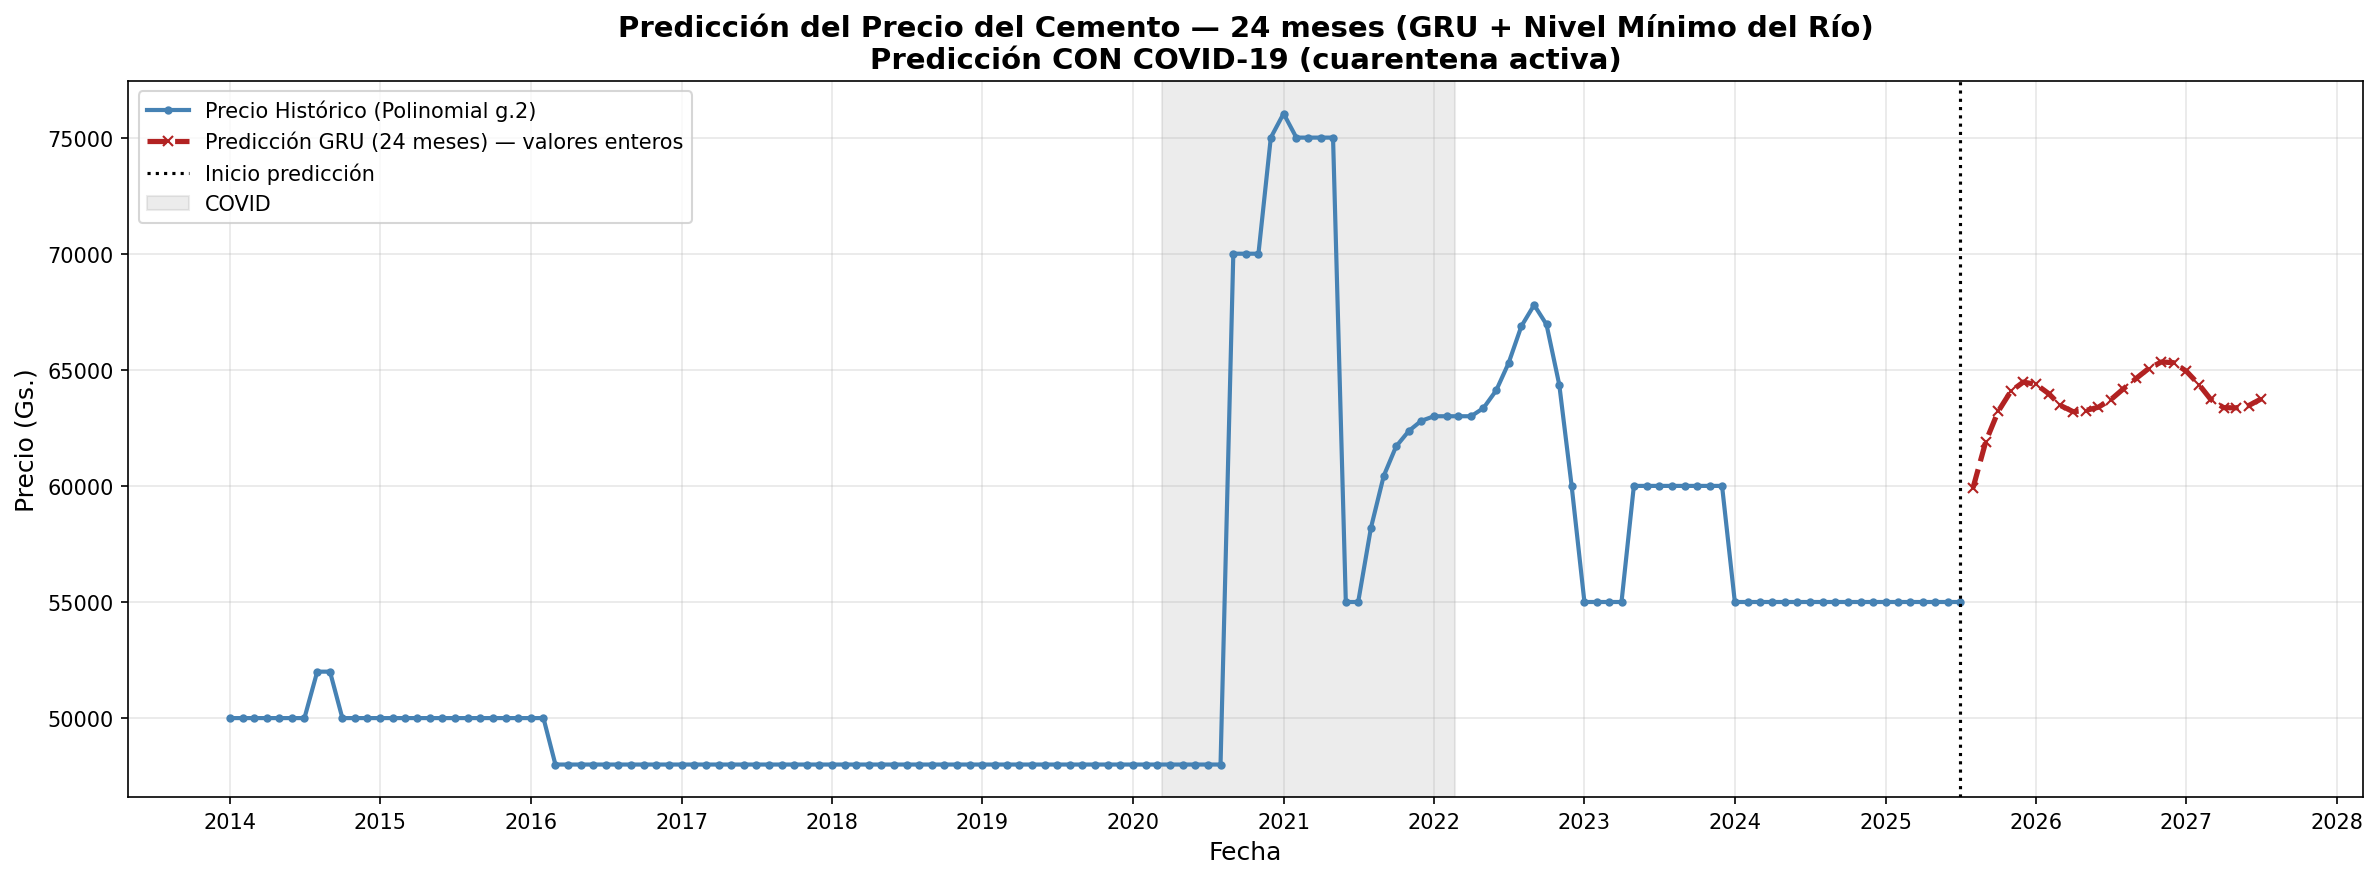
\includegraphics[width=\textwidth]{predicciones/prediccion_cemento_gru/resultados_con_covid/final_06_prediccion_futura_completa.png}
    \caption{Pronóstico GRU del precio del cemento a 24 meses --- escenario con pandemia: serie histórica y proyección.}
    \label{fig:gru_cemento_pred_con_covid}
\end{figure}

\begin{figure}[htbp]
    \centering
    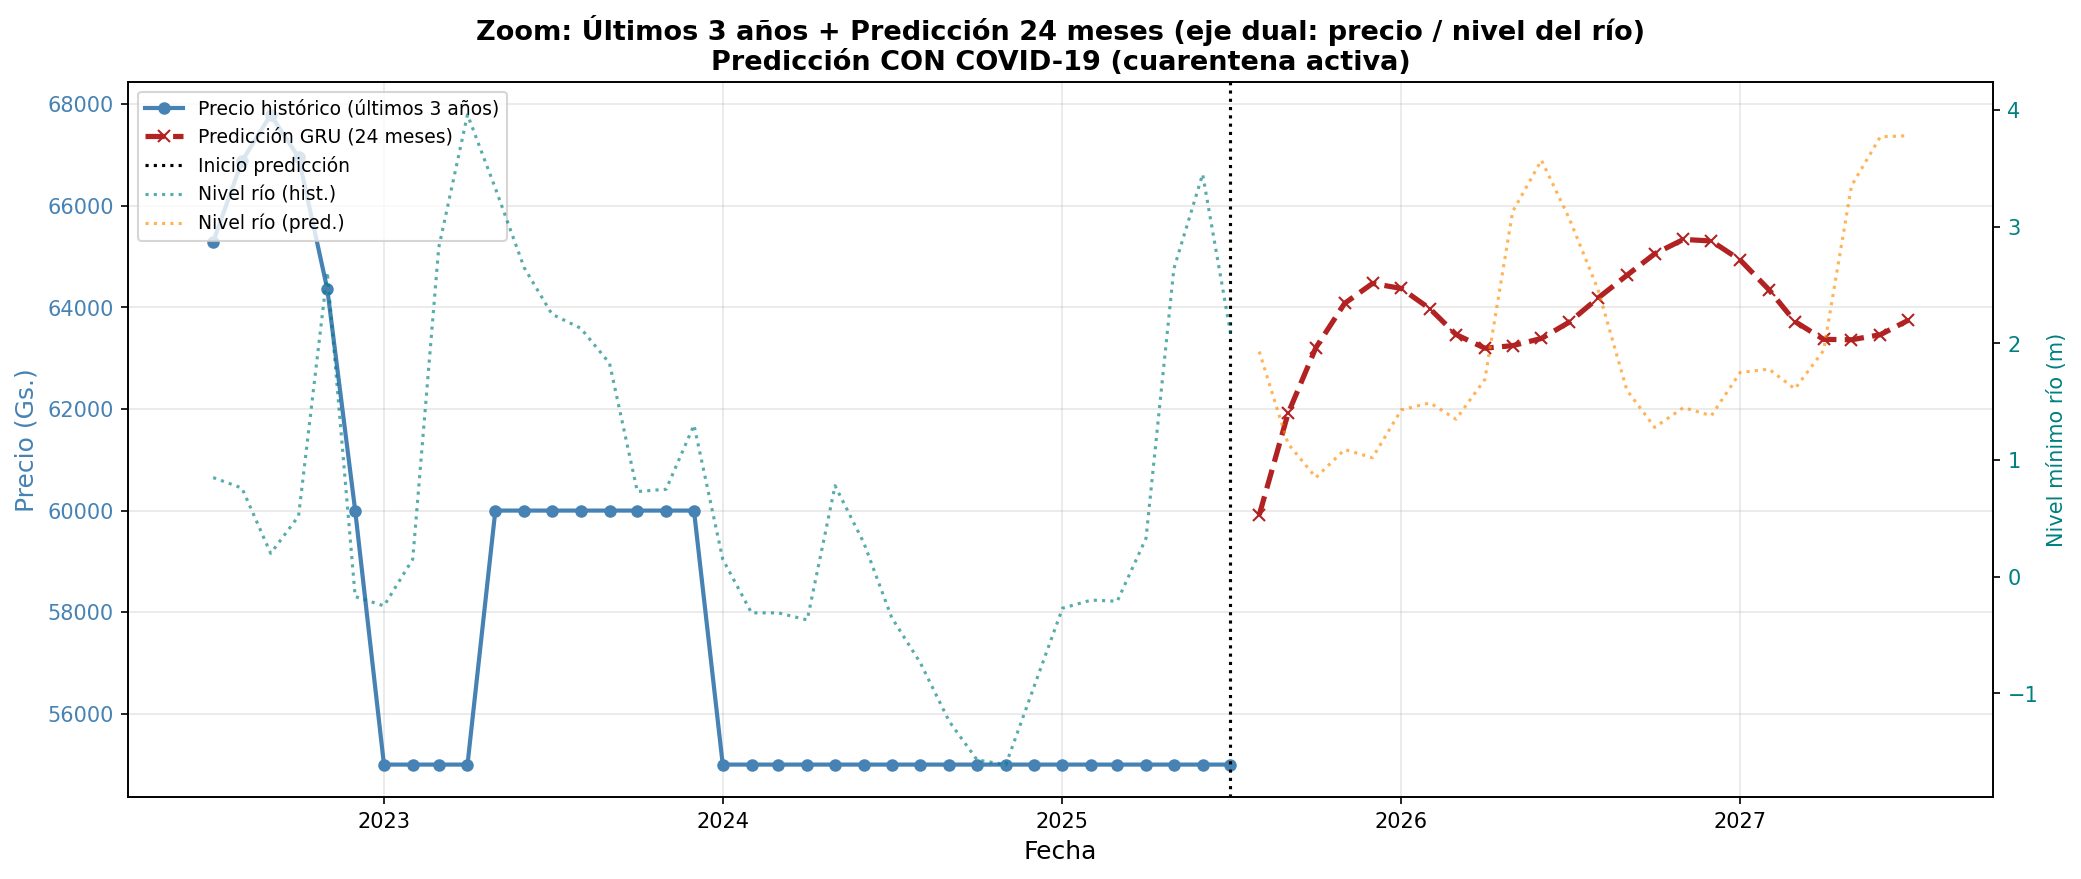
\includegraphics[width=\textwidth]{predicciones/prediccion_cemento_gru/resultados_con_covid/final_07_prediccion_zoom_dual.png}
    \caption{Zoom sobre la transición entre datos observados y pronóstico GRU del cemento --- escenario con pandemia.}
    \label{fig:gru_cemento_zoom_con_covid}
\end{figure}

\begin{figure}[htbp]
    \centering
    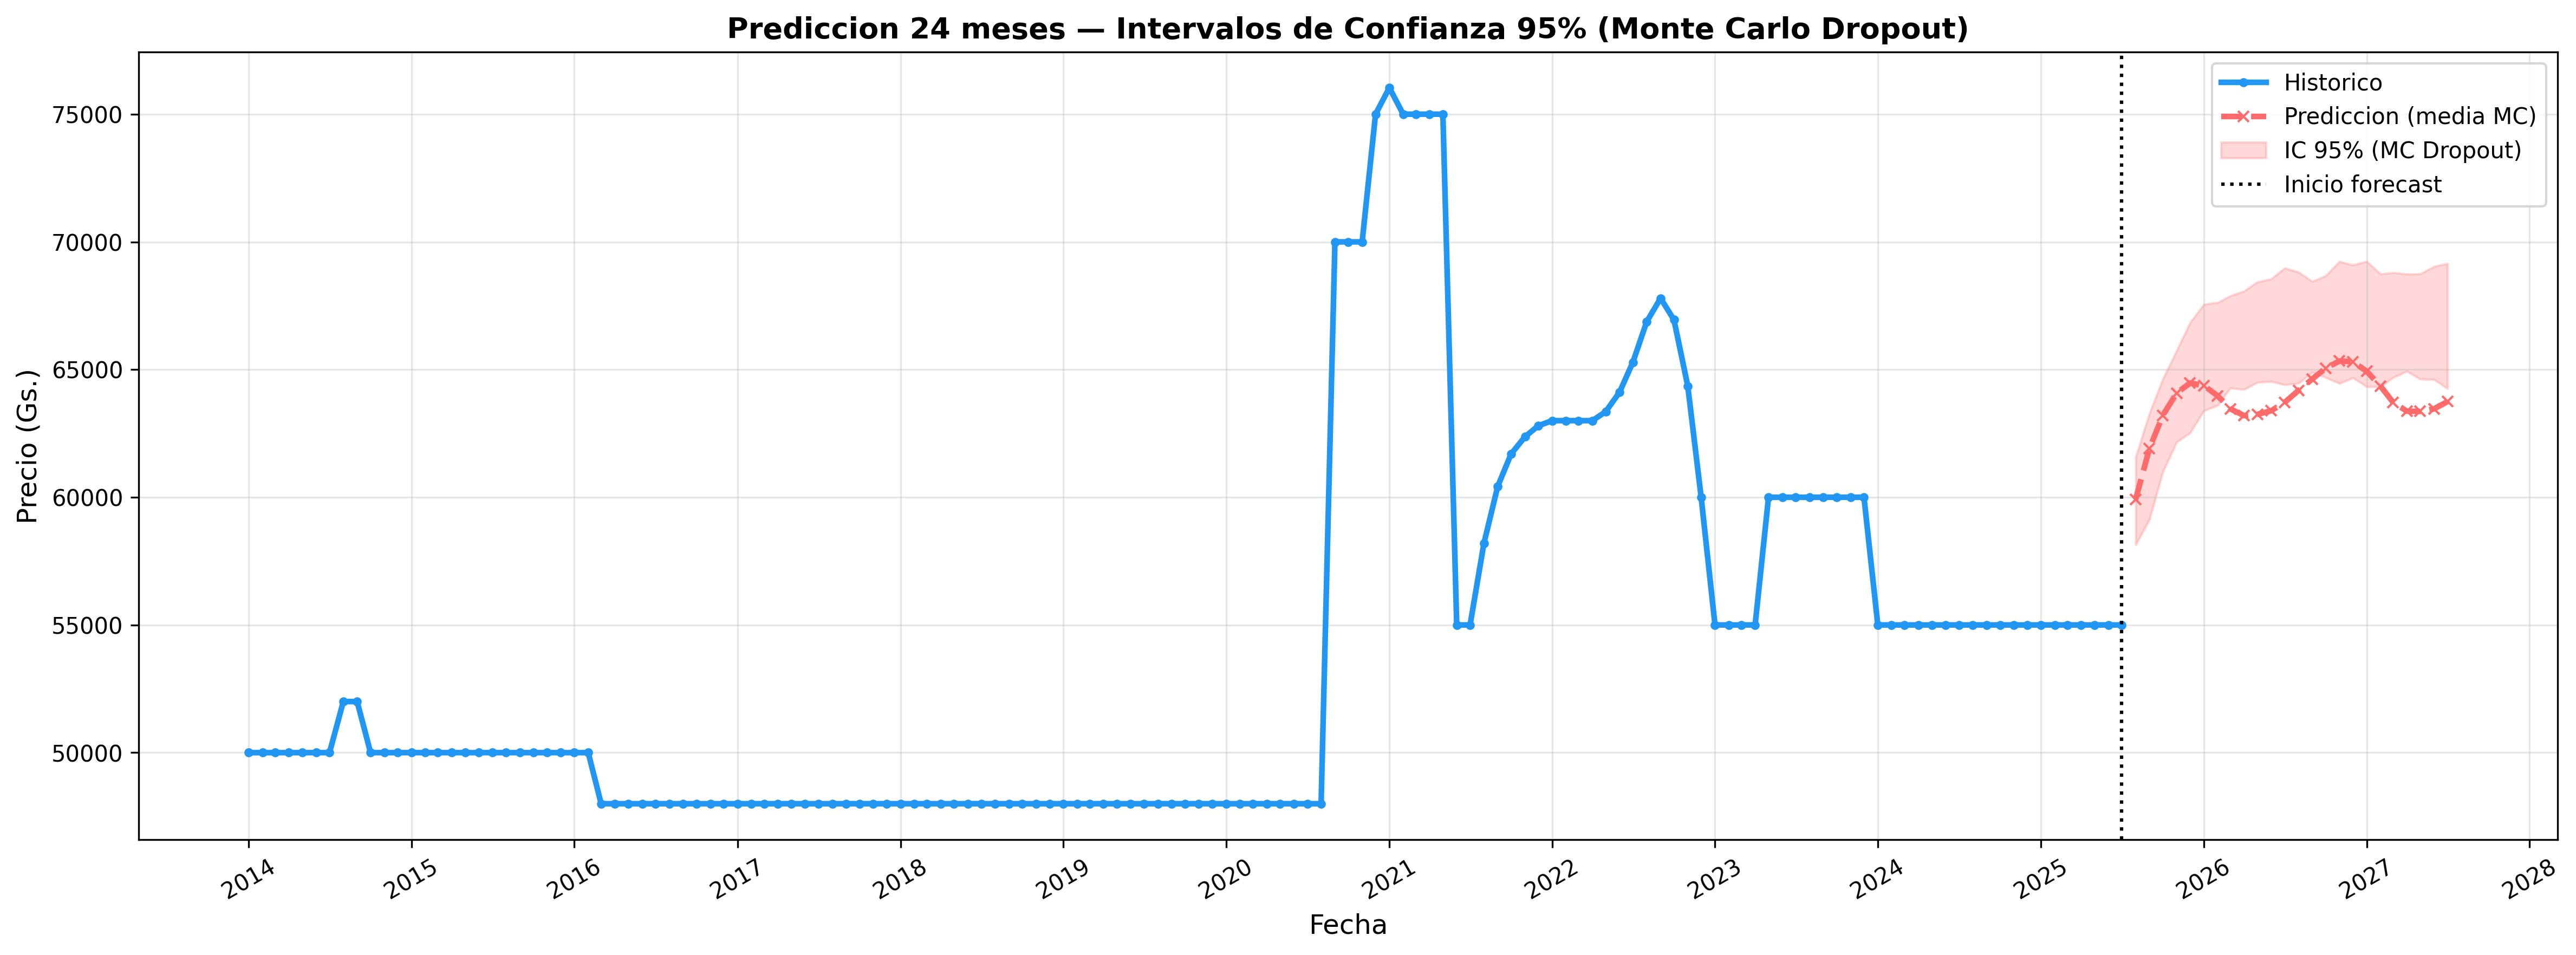
\includegraphics[width=\textwidth]{predicciones/prediccion_cemento_gru/resultados_con_covid/forecast_ic_monte_carlo.png}
    \caption{IC Monte Carlo Dropout del pronóstico GRU para cemento --- escenario con pandemia.}
    \label{fig:gru_cemento_ic_con_covid}
\end{figure}

\justify
Bajo el escenario con efecto pandémico, el modelo GRU proyecta para el cemento precios considerablemente inferiores al escenario sin pandemia, con el rango completo entre Gs.~46.048 y Gs.~53.874. La diferencia es sustancial: mientras que sin pandemia el precio asciende hasta Gs.~61.845, con pandemia el modelo proyecta una trayectoria descendente que alcanza un mínimo de Gs.~46.048. La GRU interpreta la señal de cuarentena activa como un factor de contracción de la demanda, lo que contrasta con la interpretación alcista que el LSTM asignó al mismo escenario. Este resultado es un hallazgo relevante de la comparación entre arquitecturas: ambas redes aprendieron aspectos diferentes del fenómeno pandémico a partir de los mismos datos históricos.

% ============================================================
% 4.4.2 — LADRILLO GRU
% ============================================================
\clearpage
\subsection{Predicción del Precio del Ladrillo}

\justify
Para el ladrillo, la búsqueda con Optuna fue realizada de forma independiente en cada escenario y ambos convergieron a la misma configuración GRU unidireccional con 64 unidades ocultas y 13.889 parámetros entrenables. A continuación se presenta cada escenario por separado.

% ------ LADRILLO GRU SIN COVID ------
\clearpage
\subsubsection{Escenario sin Efecto Pandémico}

\paragraph{Hiperparámetros y Arquitectura}

\justify
La búsqueda con Optuna (261 ensayos, 194,9 min) identificó una arquitectura GRU unidireccional con 64 unidades ocultas y ventana de entrada (\textit{lookback}) de 3 meses. El optimizador Adam con $\eta = 0{,}008441$ y \textit{weight decay} de $1{,}04 \times 10^{-6}$ resultó la configuración más eficiente, junto con \textit{batch size} de 8, \textit{dropout} de 0{,}05, \textit{dropout} recurrente de 0{,}2 y \textit{scheduler} StepLR. La arquitectura totaliza 13.889 parámetros entrenables. La Tabla~\ref{tab:gru_ladrillo_sc_arq} resume los hiperparámetros.

\begin{table}[htbp]
    \centering
    \caption{Hiperparámetros del modelo GRU para ladrillo --- escenario sin pandemia (Optuna: 261 ensayos, 194{,}9 min).}
    \label{tab:gru_ladrillo_sc_arq}
    \begin{tabular}{ll}
        \toprule
        \textbf{Hiperparámetro} & \textbf{Valor} \\
        \midrule
        Capas GRU              & 1 (unidireccional) \\
        Unidades ocultas       & 64 \\
        Lookback               & 3 meses \\
        Optimizador            & Adam ($\eta=0{,}008441$, WD $=1{,}04 \times 10^{-6}$) \\
        Batch size             & 8 \\
        Dropout / Rec.\ dropout & 0{,}05 / 0{,}2 \\
        Scheduler              & StepLR \\
        Parámetros entrenables & 13.889 \\
        \bottomrule
    \end{tabular}
\end{table}

\paragraph{Curva de Aprendizaje}

\justify
El modelo GRU del ladrillo para el escenario sin pandemia convergió en 62 épocas con \textit{early stopping}. La Figura~\ref{fig:gru_ladrillo_curva_sc} muestra las curvas de pérdida. La convergencia en pocas épocas es consistente con la tasa de aprendizaje relativamente alta ($\eta=0{,}008441$) del optimizador Adam, que permite alcanzar rápidamente una región de mínimo local, mientras que el \textit{scheduler} StepLR reduce gradualmente la tasa para afinar el ajuste en las épocas finales.

\begin{figure}[htbp]
    \centering
    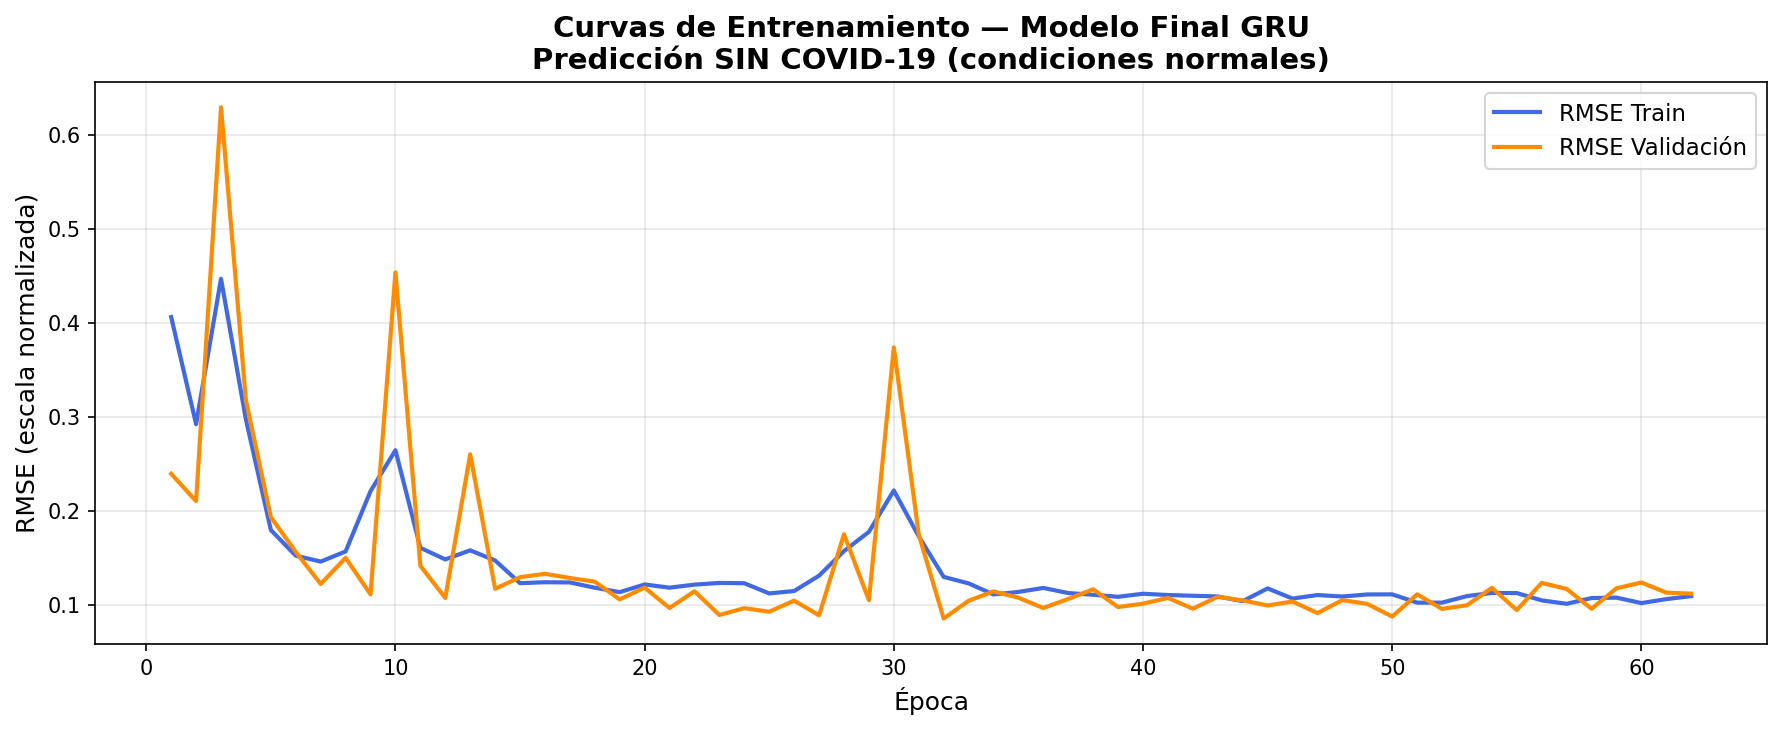
\includegraphics[width=\textwidth]{predicciones/prediccion_ladrillo_gru/resultados_sin_covid/final_01_curvas_entrenamiento.png}
    \caption{Curvas de aprendizaje del modelo GRU para ladrillo --- escenario sin pandemia.}
    \label{fig:gru_ladrillo_curva_sc}
\end{figure}

\paragraph{Métricas de Evaluación}

\begin{table}[htbp]
    \centering
    \caption{Desempeño del modelo GRU para ladrillo --- escenario sin pandemia: RMSE en train, val y test.}
    \label{tab:gru_ladrillo_sc_metricas}
    \begin{tabular}{lrrr}
        \toprule
        \textbf{Métrica} & \textbf{Train} & \textbf{Val} & \textbf{Test} \\
        \midrule
        RMSE (Gs.) & 15{,}56 & 11{,}53 & 11{,}88 \\
        \bottomrule
    \end{tabular}
\end{table}

\justify
El RMSE de validación (Gs.~11{,}53) y el de prueba (Gs.~11{,}88) son coherentes entre sí, lo que indica ausencia de sobreajuste. El RMSE de entrenamiento (Gs.~15{,}56) es mayor porque el período histórico completo de entrenamiento contiene mayor variabilidad que el período de prueba.

\paragraph{Evaluación sobre el Conjunto de Prueba}

\begin{figure}[htbp]
    \centering
    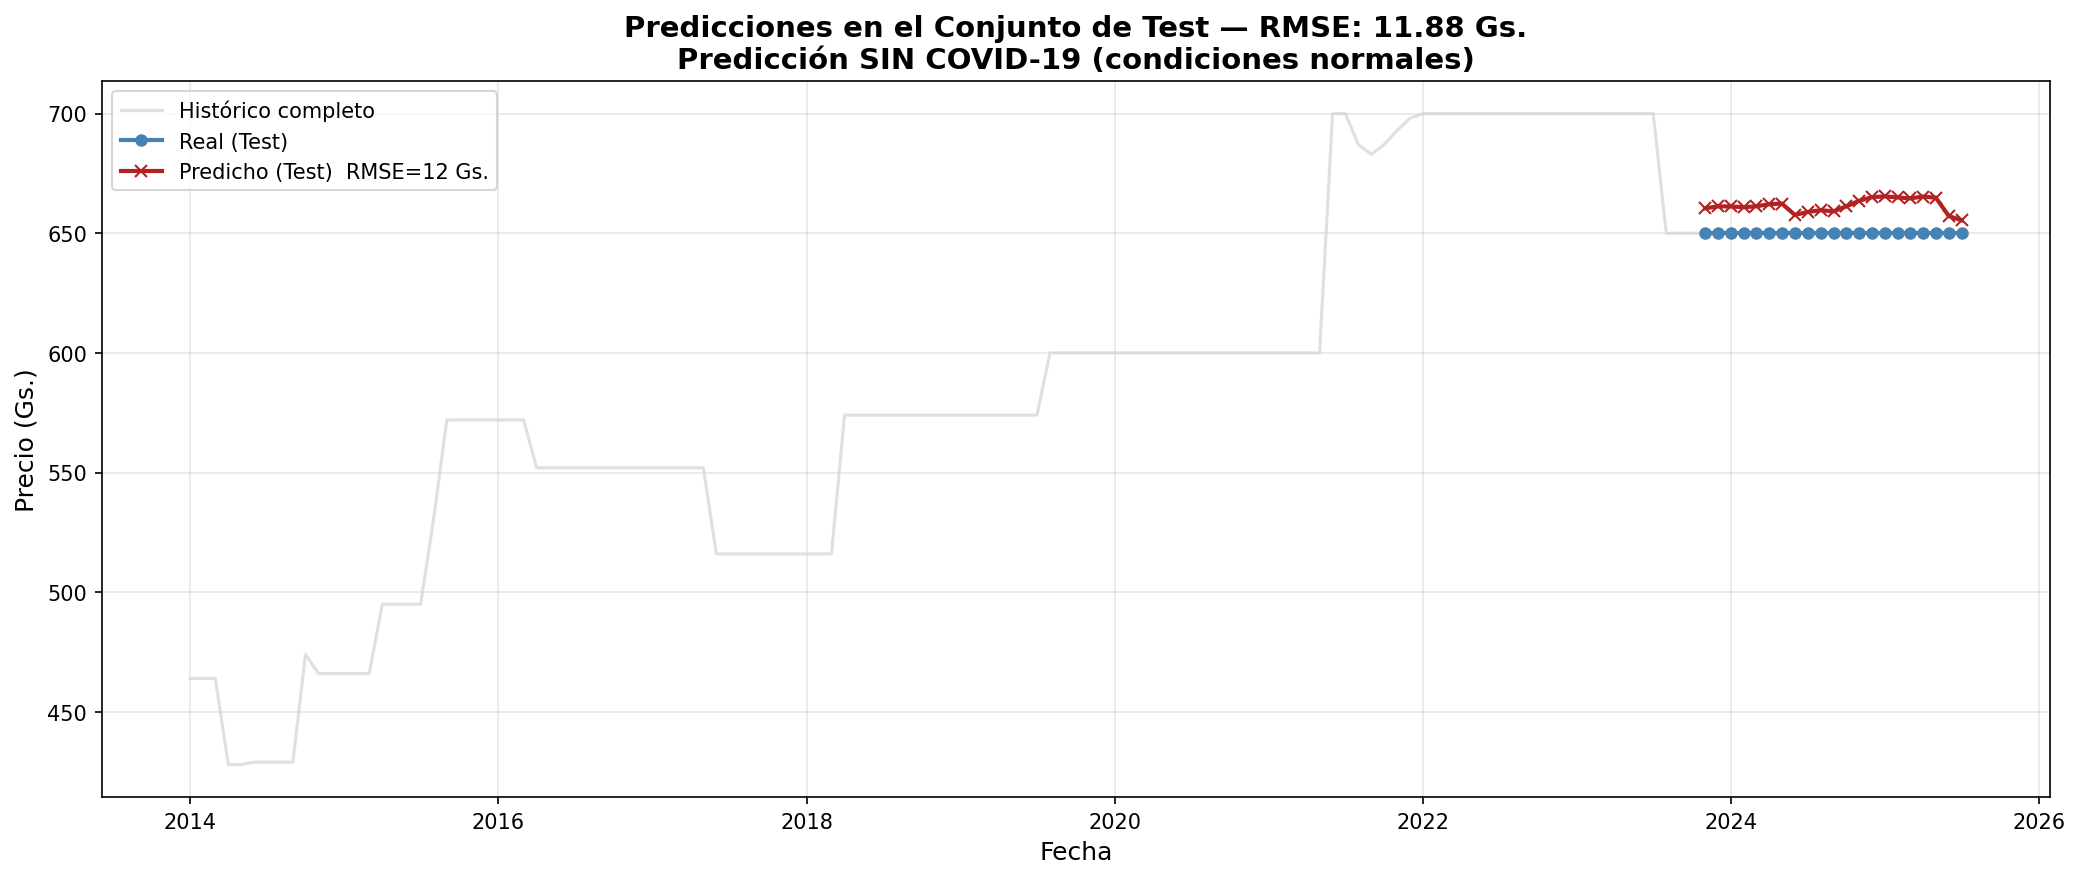
\includegraphics[width=\textwidth]{predicciones/prediccion_ladrillo_gru/resultados_sin_covid/final_02_prediccion_test_serie.png}
    \caption{Predicción GRU vs.\ valores reales del precio del ladrillo --- escenario sin pandemia, conjunto de prueba.}
    \label{fig:gru_ladrillo_test_sc}
\end{figure}

\begin{figure}[htbp]
    \centering
    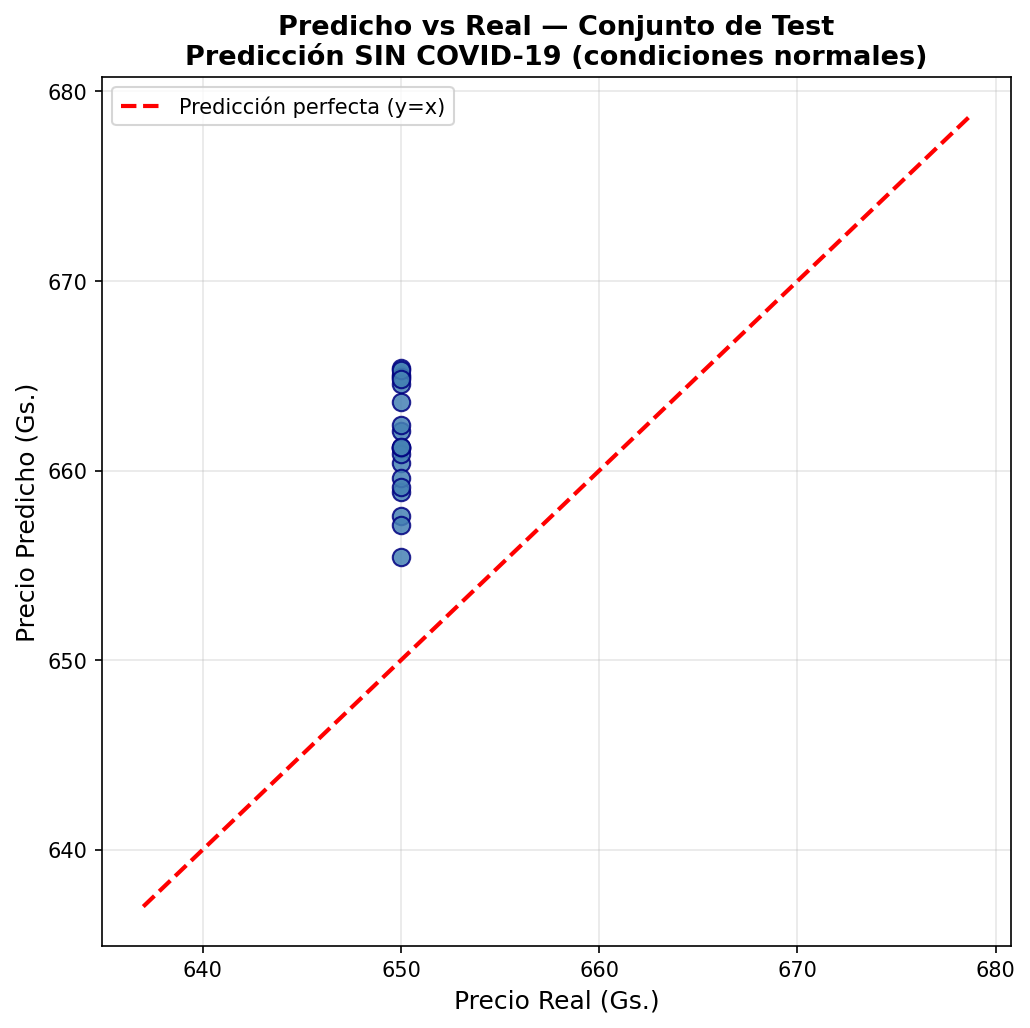
\includegraphics[width=0.8\textwidth]{predicciones/prediccion_ladrillo_gru/resultados_sin_covid/final_03_scatter_test.png}
    \caption{Diagrama de dispersión: precio predicho vs.\ real del ladrillo --- escenario sin pandemia (GRU).}
    \label{fig:gru_ladrillo_scatter_sc}
\end{figure}

\begin{figure}[htbp]
    \centering
    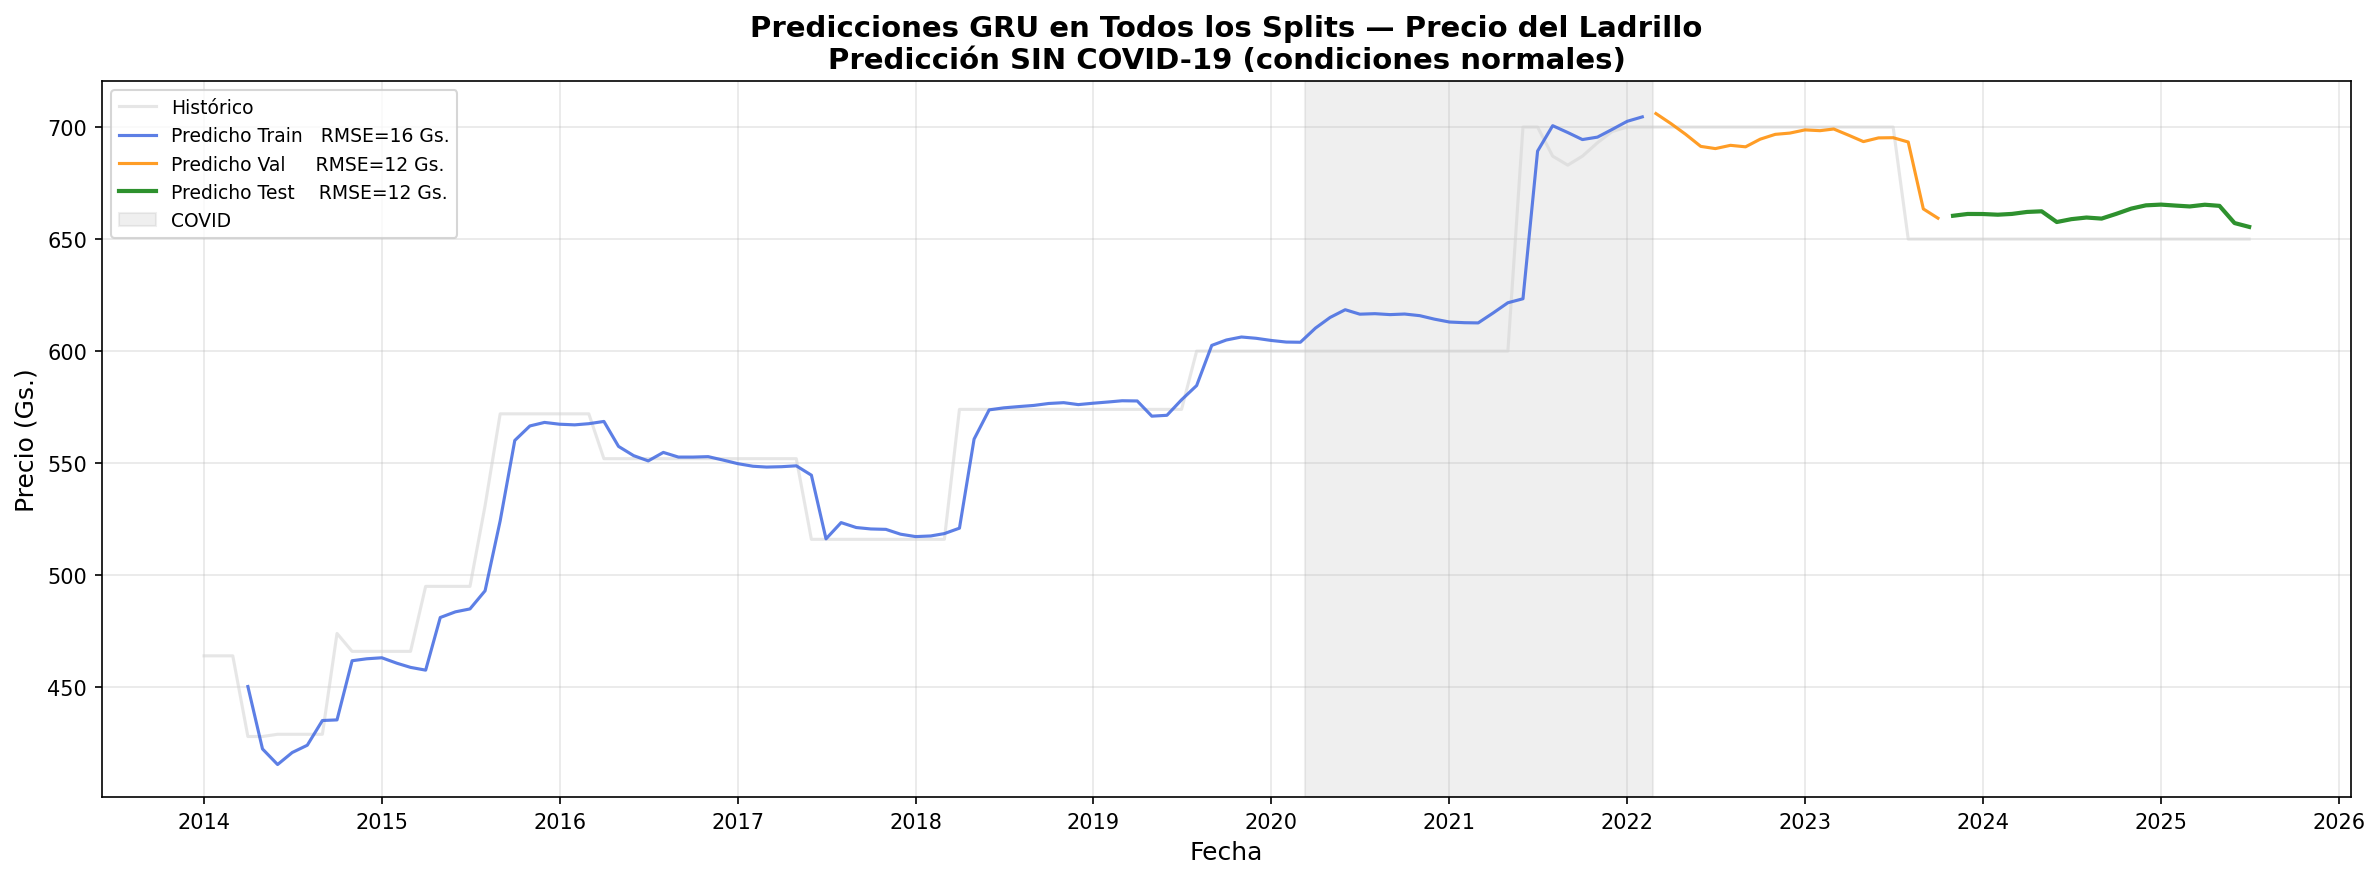
\includegraphics[width=\textwidth]{predicciones/prediccion_ladrillo_gru/resultados_sin_covid/final_05_todos_splits.png}
    \caption{Ajuste del modelo GRU del ladrillo sobre las tres particiones --- escenario sin pandemia.}
    \label{fig:gru_ladrillo_splits_sc}
\end{figure}

\clearpage
\paragraph{Análisis de Residuos}

\begin{figure}[htbp]
    \centering
    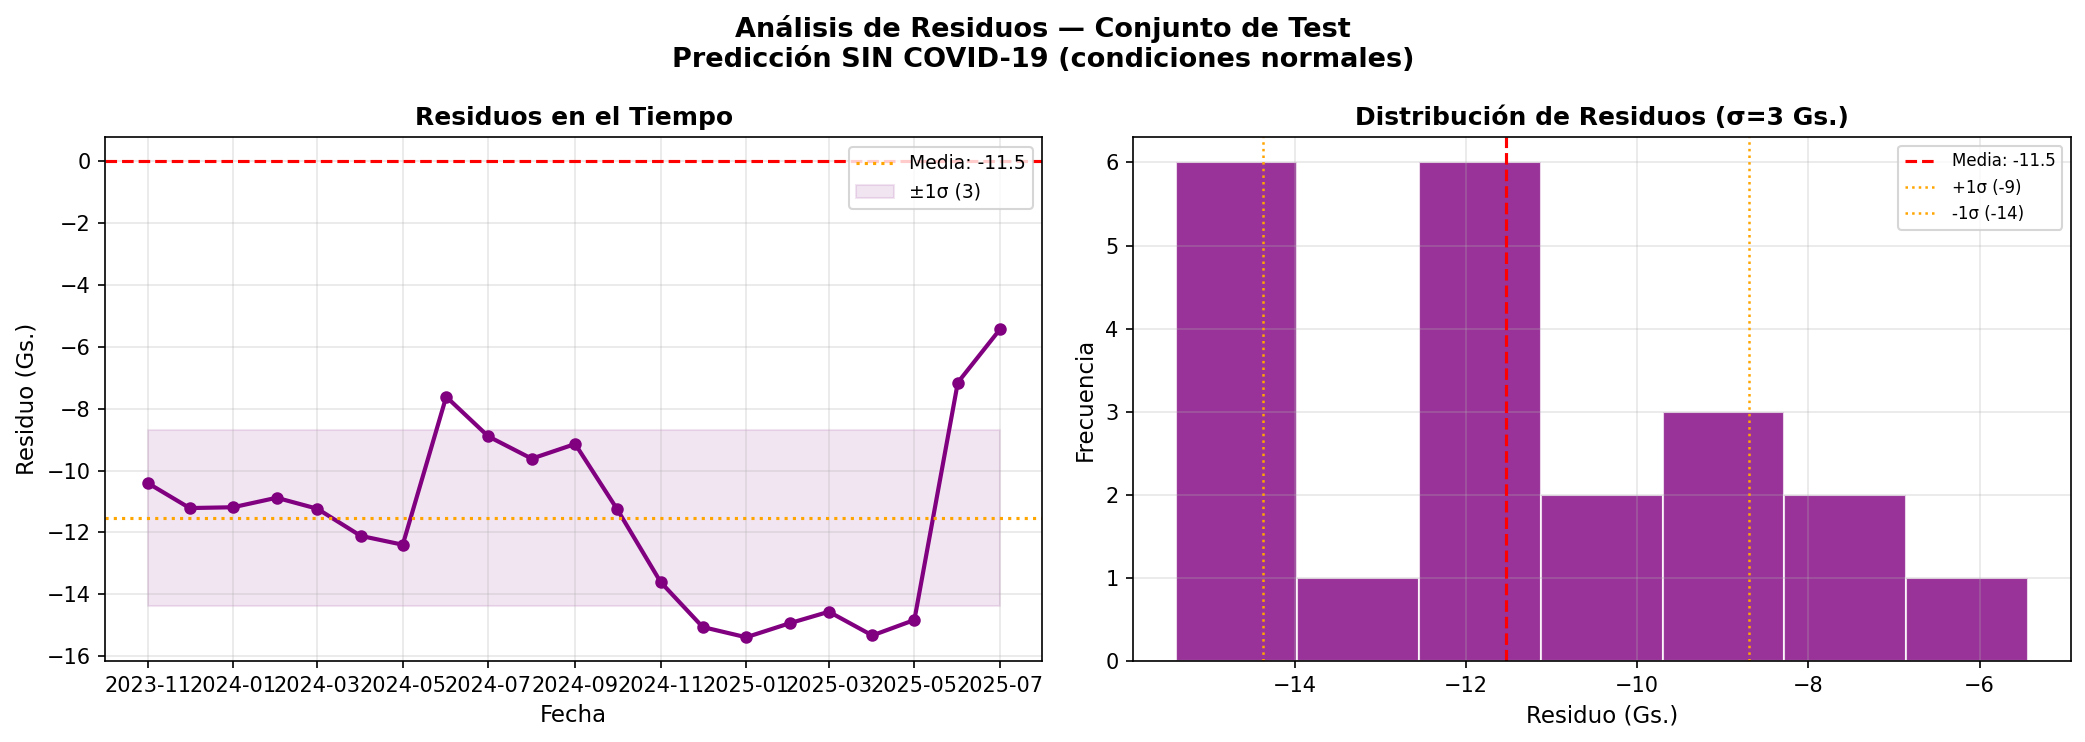
\includegraphics[width=\textwidth]{predicciones/prediccion_ladrillo_gru/resultados_sin_covid/final_04_residuos.png}
    \caption{Residuos del modelo GRU para ladrillo --- escenario sin pandemia, conjunto de prueba.}
    \label{fig:gru_ladrillo_res_sc}
\end{figure}

\begin{figure}[htbp]
    \centering
    \includegraphics[width=0.8\textwidth]{predicciones/prediccion_ladrillo_gru/resultados_sin_covid/residuos_histograma.png}
    \caption{Histograma de residuos del modelo GRU para ladrillo --- escenario sin pandemia.}
    \label{fig:gru_ladrillo_reshist_sc}
\end{figure}

\begin{figure}[htbp]
    \centering
    \includegraphics[width=\textwidth]{predicciones/prediccion_ladrillo_gru/resultados_sin_covid/residuos_acf_pacf.png}
    \caption{ACF y PACF de los residuos del modelo GRU para ladrillo --- escenario sin pandemia.}
    \label{fig:gru_ladrillo_acf_sc}
\end{figure}

\justify
El test de Ljung-Box sobre los residuos del conjunto de prueba no rechaza la hipótesis nula de ausencia de autocorrelación serial en ninguno de los rezagos evaluados: $p=0{,}442$ a 10 rezagos y $p=0{,}081$ a 20 rezagos, ambos superiores al umbral de 0{,}05. Este resultado confirma que los residuos se comportan como ruido blanco y que la estructura temporal de la serie ha sido capturada adecuadamente, un resultado notable para el modelo más compacto del estudio.

\clearpage
\paragraph{Pronóstico a 24 Meses}

\begin{figure}[htbp]
    \centering
    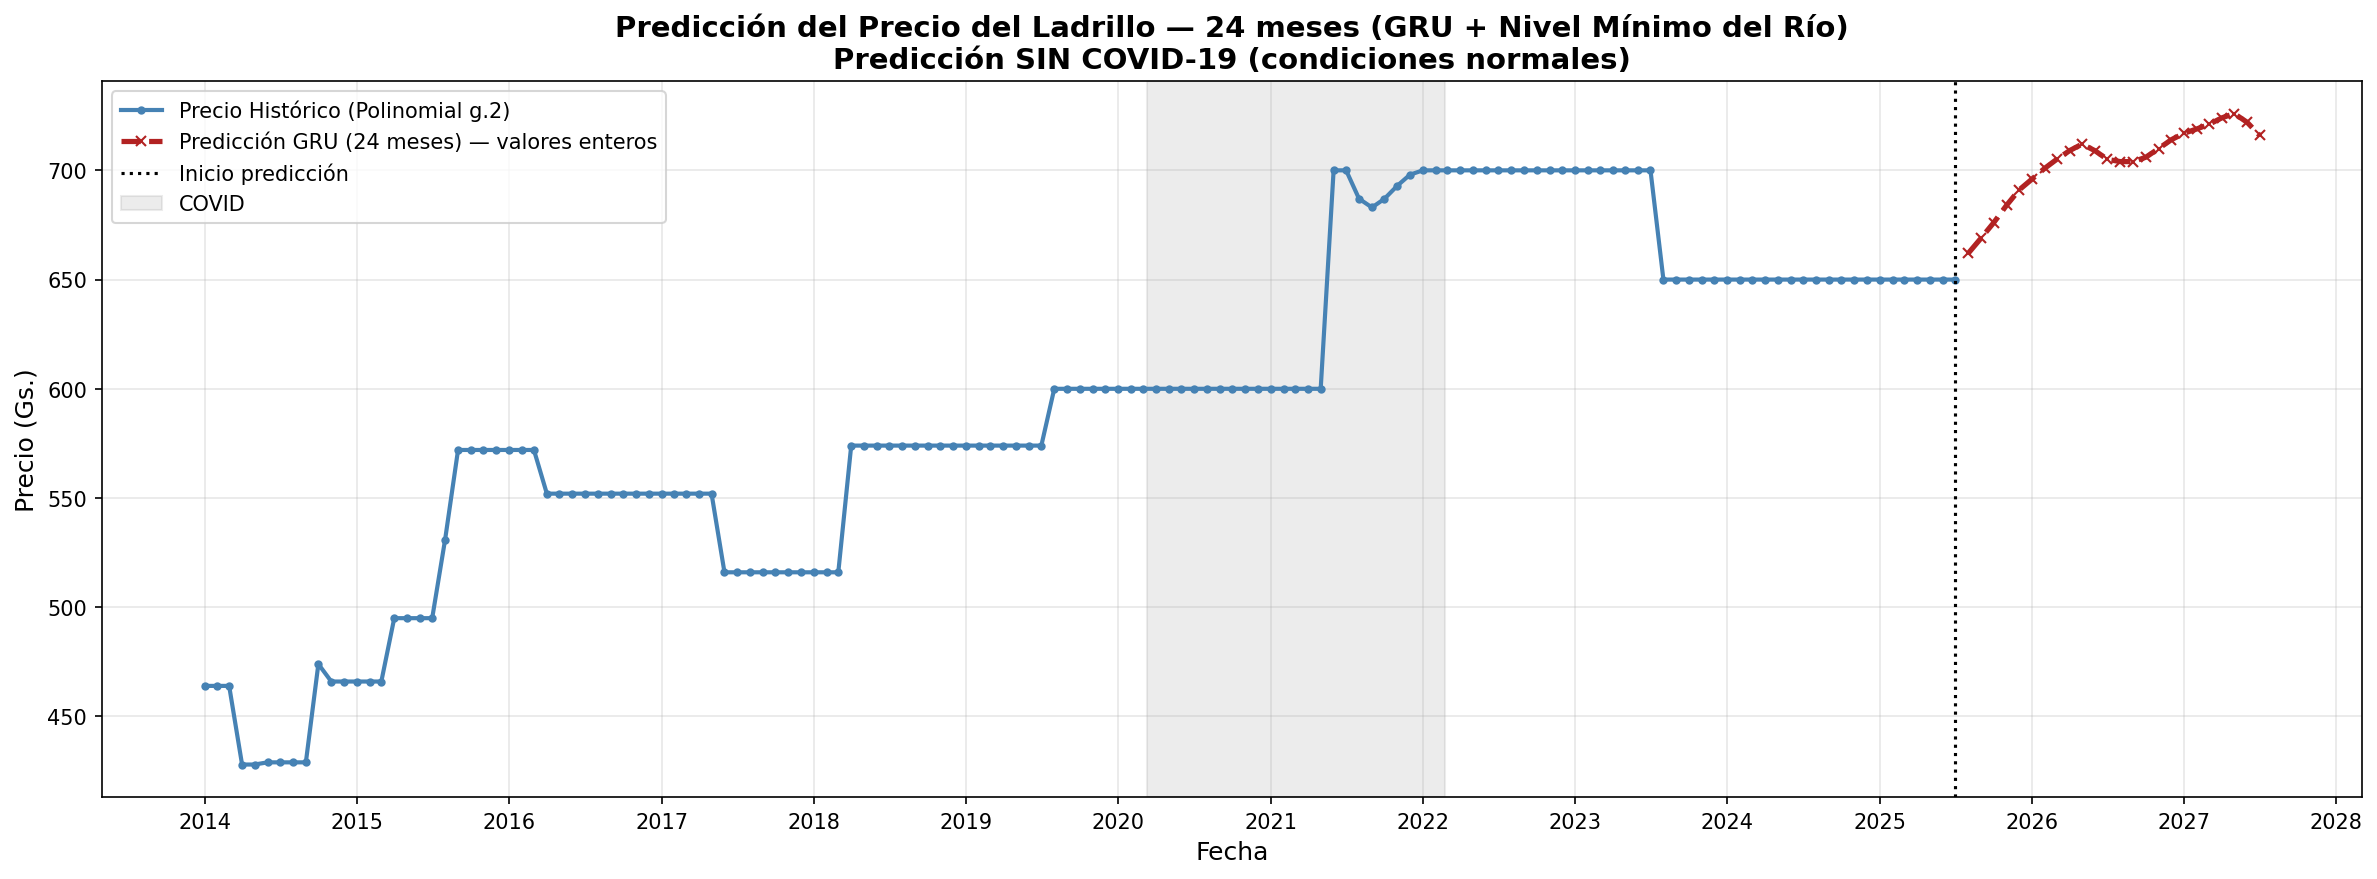
\includegraphics[width=\textwidth]{predicciones/prediccion_ladrillo_gru/resultados_sin_covid/final_06_prediccion_futura_completa.png}
    \caption{Pronóstico GRU del precio del ladrillo a 24 meses --- escenario sin pandemia: serie histórica y proyección.}
    \label{fig:gru_ladrillo_pred_sin_covid}
\end{figure}

\begin{figure}[htbp]
    \centering
    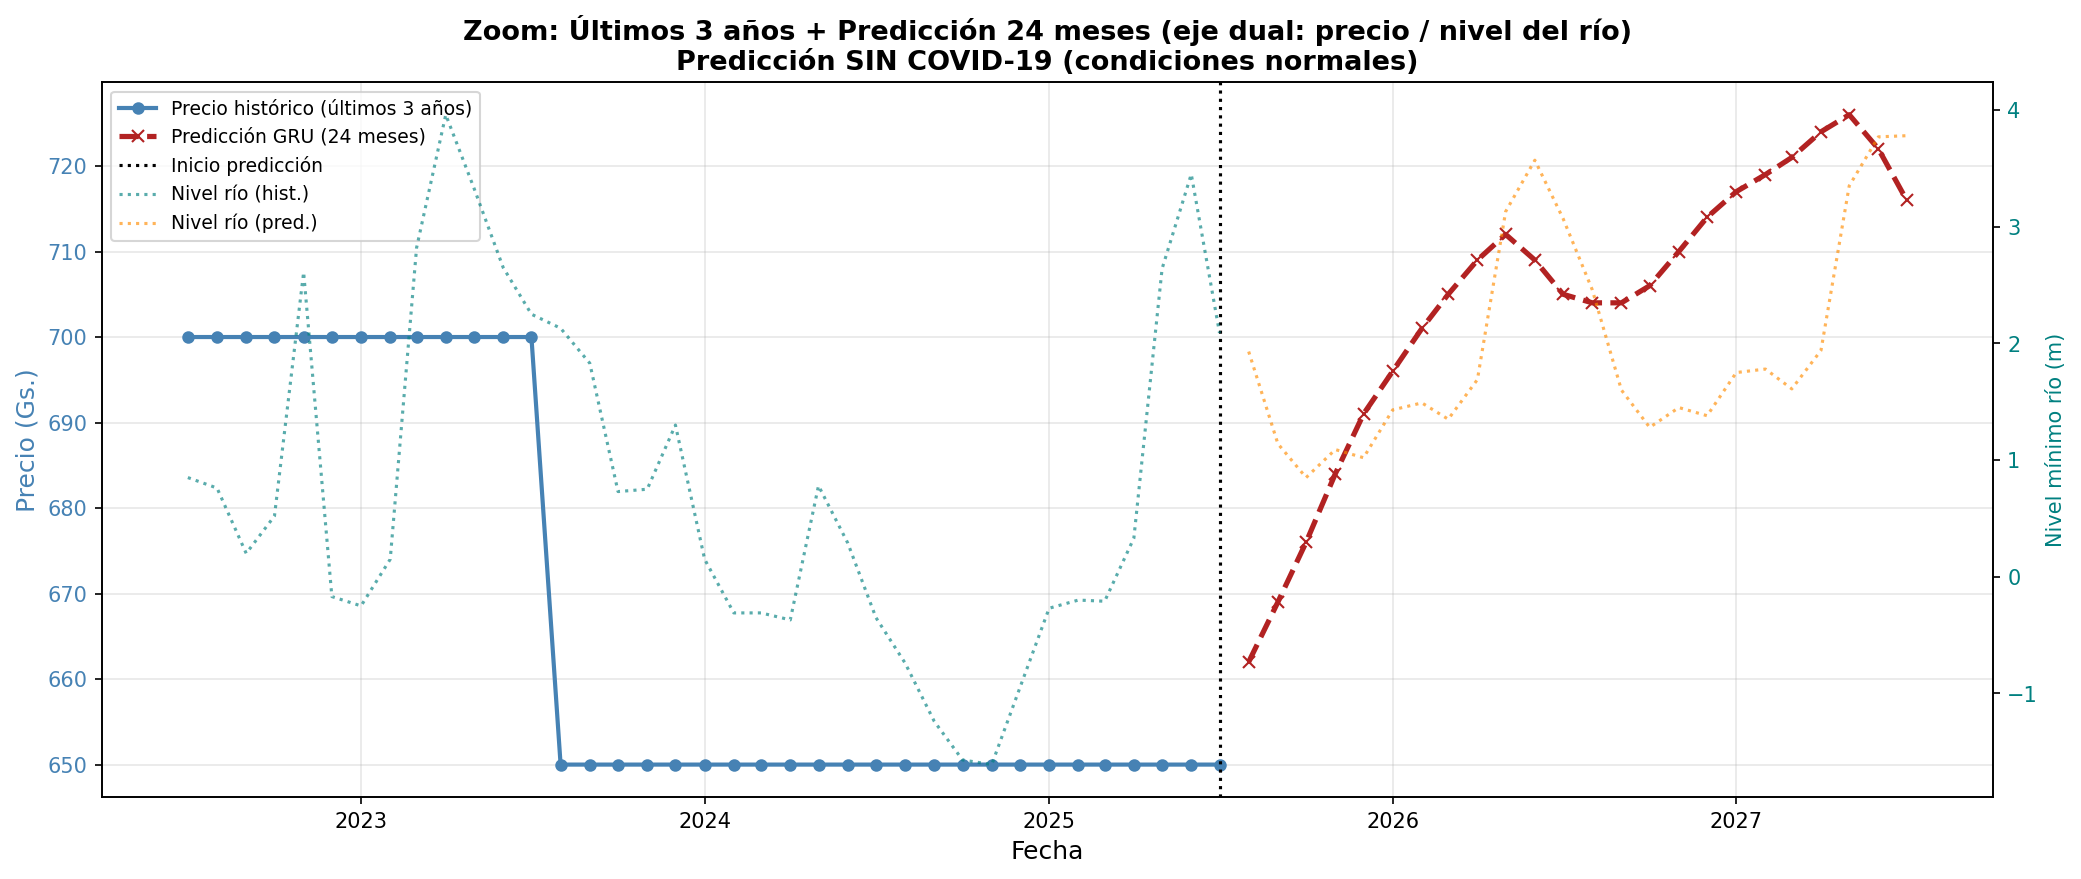
\includegraphics[width=\textwidth]{predicciones/prediccion_ladrillo_gru/resultados_sin_covid/final_07_prediccion_zoom_dual.png}
    \caption{Zoom sobre la transición entre datos observados y pronóstico GRU del ladrillo --- escenario sin pandemia.}
    \label{fig:gru_ladrillo_zoom_sin_covid}
\end{figure}

\begin{figure}[htbp]
    \centering
    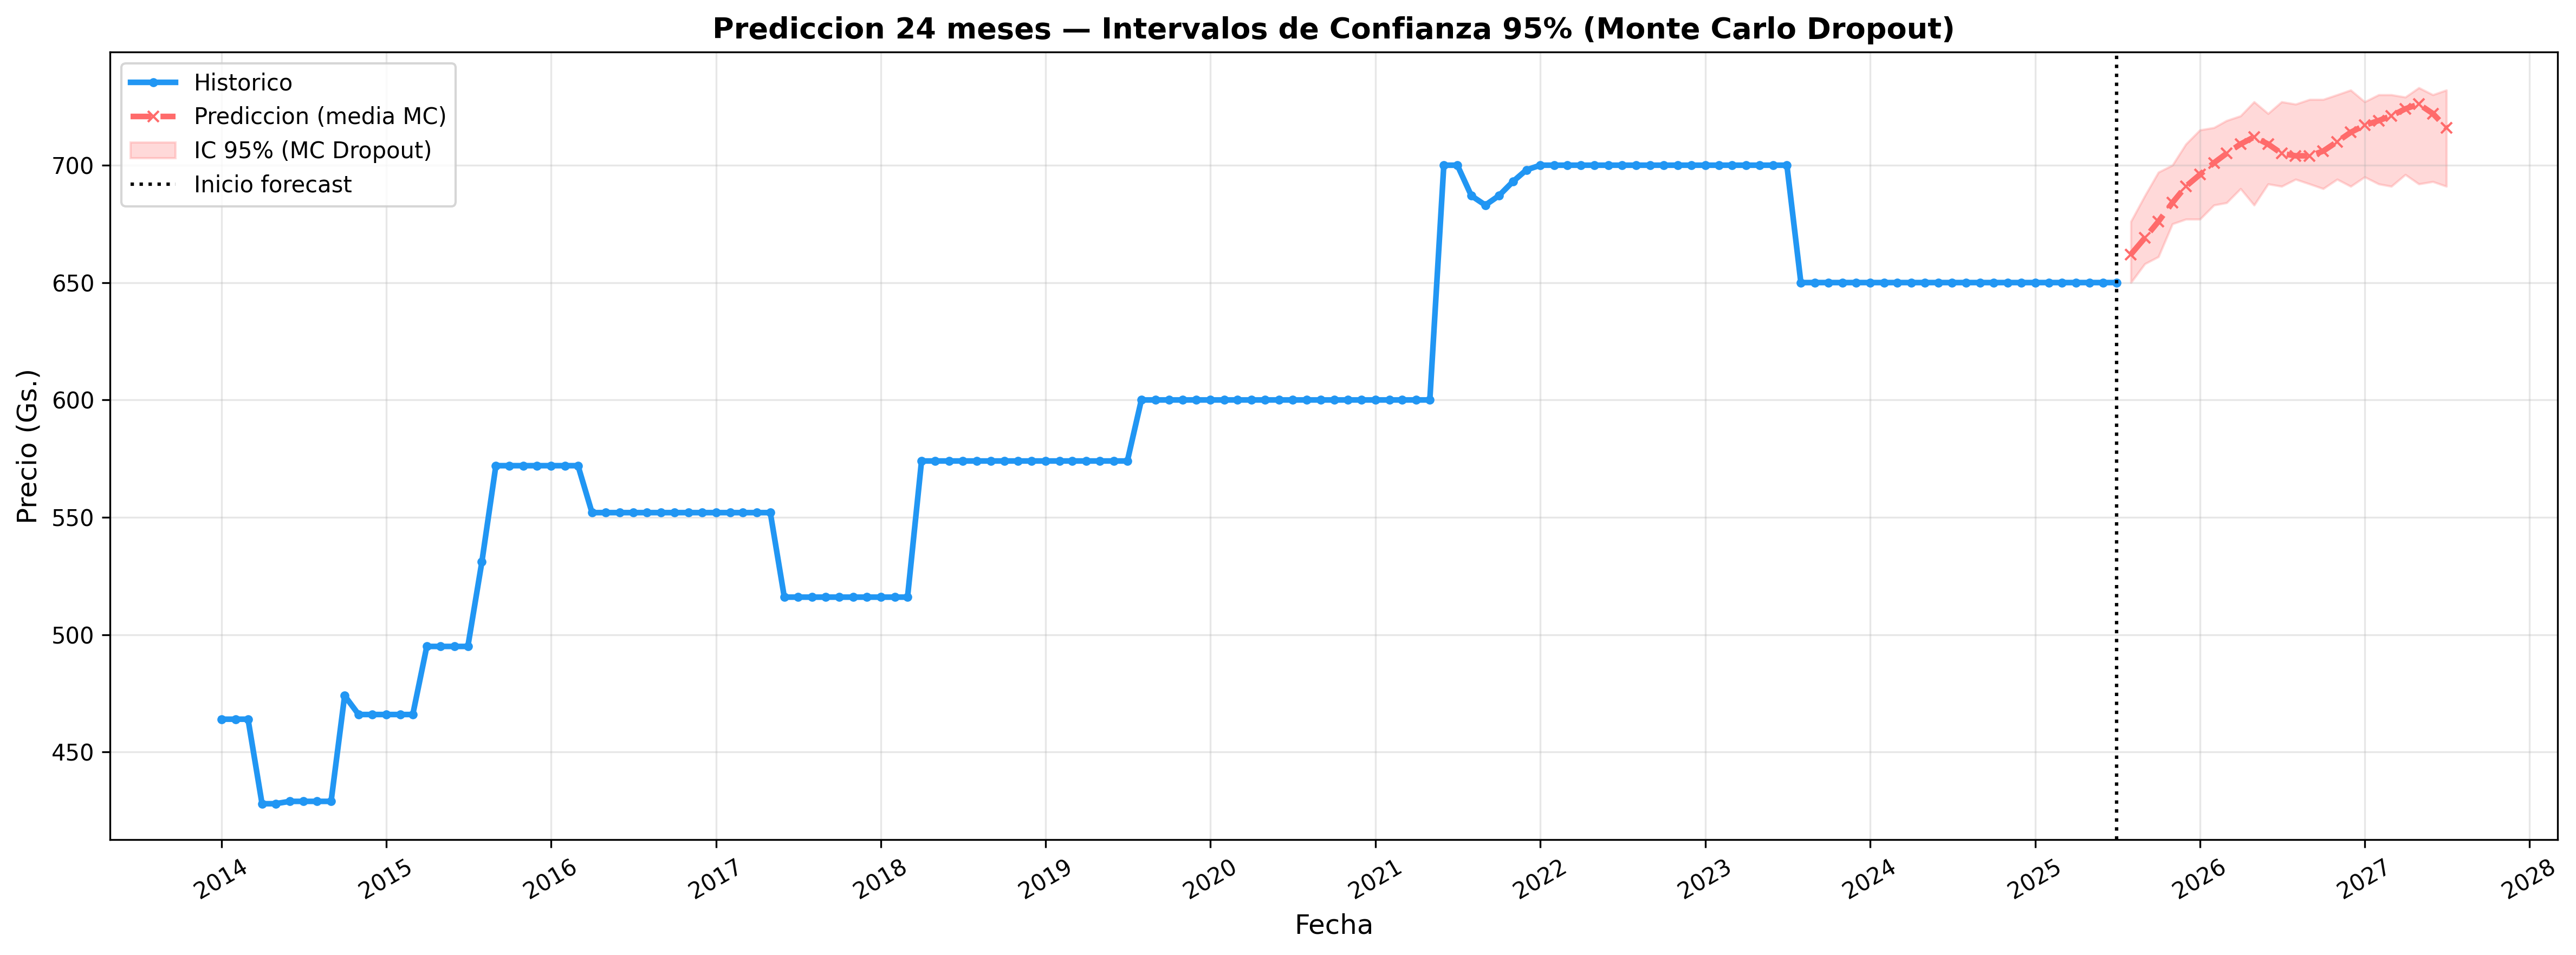
\includegraphics[width=\textwidth]{predicciones/prediccion_ladrillo_gru/resultados_sin_covid/forecast_ic_monte_carlo.png}
    \caption{IC Monte Carlo Dropout del pronóstico GRU para ladrillo --- escenario sin pandemia.}
    \label{fig:gru_ladrillo_ic_sin_covid}
\end{figure}

\justify
El modelo GRU proyecta, bajo el escenario sin pandemia, un precio del ladrillo en el rango de Gs.~662 a Gs.~726 a lo largo del horizonte de 24 meses. La amplitud del intervalo refleja la incertidumbre acumulada en las predicciones recursivas, aunque su magnitud sigue siendo moderada para una proyección de dos años.

% ------ LADRILLO GRU CON COVID ------
\clearpage
\subsubsection{Escenario con Efecto Pandémico}

\paragraph{Hiperparámetros y Arquitectura}

\justify
Para el escenario con pandemia, la búsqueda con Optuna (261 ensayos, 171,2 min) convergió a la misma configuración que el escenario sin pandemia: una GRU unidireccional con 64 unidades ocultas, Adam con $\eta = 0{,}008441$ y \textit{weight decay} $1{,}04 \times 10^{-6}$, \textit{lookback} de 3 meses, \textit{batch size} de 8, \textit{dropout} de 0{,}05, \textit{dropout} recurrente de 0{,}2 y \textit{scheduler} StepLR. Los 13.889 parámetros entrenables son idénticos al escenario sin pandemia. La Tabla~\ref{tab:gru_ladrillo_cc_arq} resume estos parámetros.

\begin{table}[htbp]
    \centering
    \caption{Hiperparámetros del modelo GRU para ladrillo --- escenario con pandemia.}
    \label{tab:gru_ladrillo_cc_arq}
    \begin{tabular}{ll}
        \toprule
        \textbf{Hiperparámetro} & \textbf{Valor} \\
        \midrule
        Capas GRU              & 1 (unidireccional) \\
        Unidades ocultas       & 64 \\
        Lookback               & 3 meses \\
        Optimizador            & Adam ($\eta=0{,}008441$, WD $=1{,}04 \times 10^{-6}$) \\
        Batch size             & 8 \\
        Dropout / Rec.\ dropout & 0{,}05 / 0{,}2 \\
        Scheduler              & StepLR \\
        Parámetros entrenables & 13.889 \\
        \bottomrule
    \end{tabular}
\end{table}

\paragraph{Curva de Aprendizaje}

\begin{figure}[htbp]
    \centering
    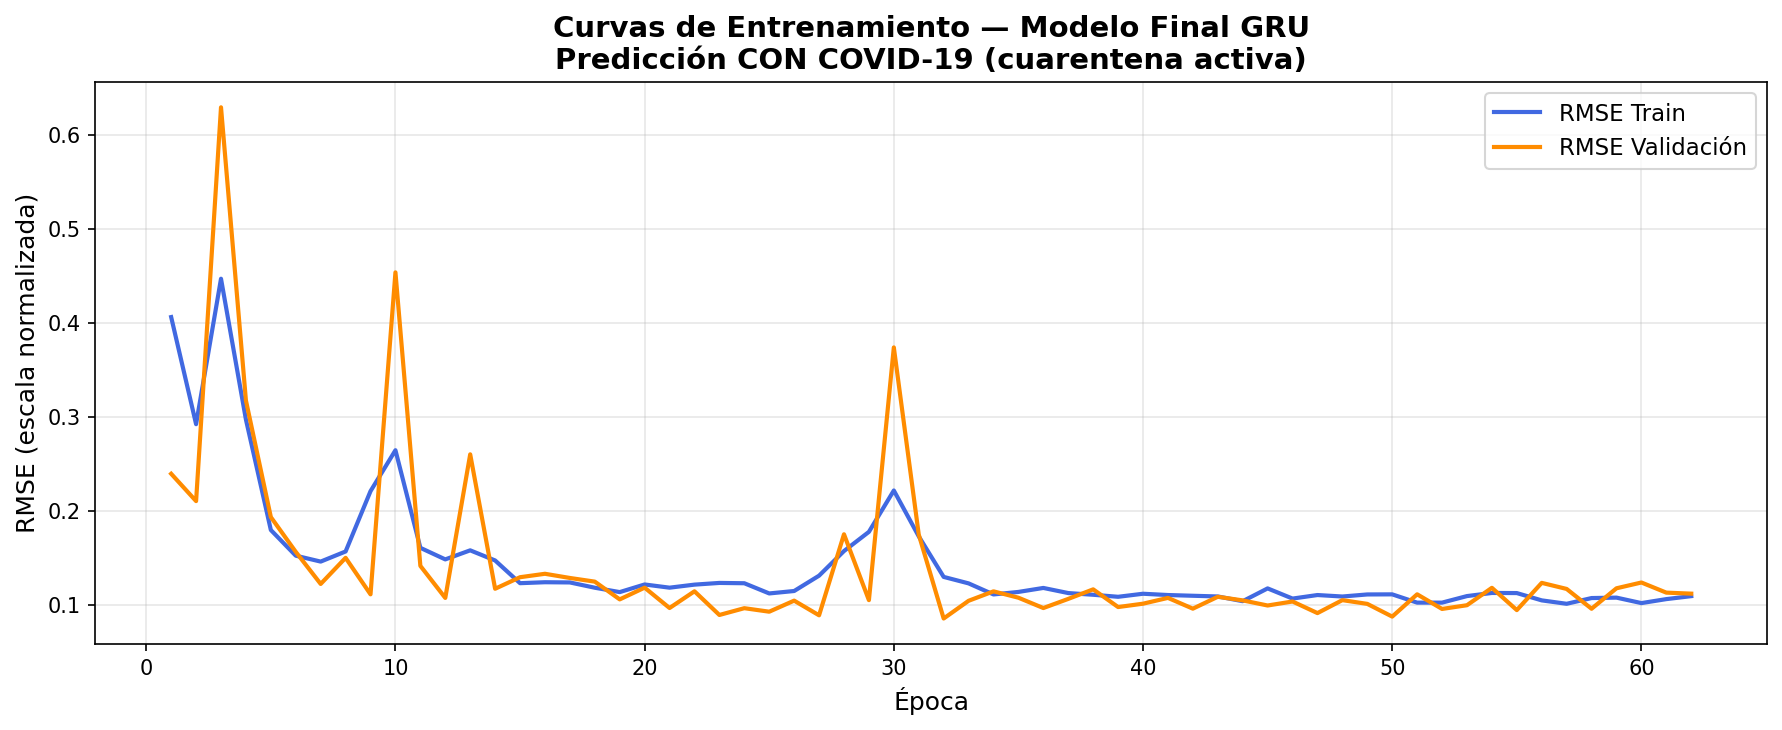
\includegraphics[width=\textwidth]{predicciones/prediccion_ladrillo_gru/resultados_con_covid/final_01_curvas_entrenamiento.png}
    \caption{Curvas de aprendizaje del modelo GRU para ladrillo --- escenario con pandemia.}
    \label{fig:gru_ladrillo_curva_cc}
\end{figure}

\paragraph{Métricas de Evaluación}

\begin{table}[htbp]
    \centering
    \caption{Desempeño del modelo GRU para ladrillo --- escenario con pandemia: RMSE en train, val y test.}
    \label{tab:gru_ladrillo_cc_metricas}
    \begin{tabular}{lrrr}
        \toprule
        \textbf{Métrica} & \textbf{Train} & \textbf{Val} & \textbf{Test} \\
        \midrule
        RMSE (Gs.) & 15{,}56 & 11{,}53 & 11{,}88 \\
        \bottomrule
    \end{tabular}
\end{table}

\justify
El RMSE de prueba del escenario con pandemia (Gs.~11{,}88) es idéntico al del escenario sin pandemia, resultado esperable dado que la búsqueda de hiperparámetros convergió a la misma configuración. El RMSE de validación de Gs.~11{,}53 también coincide, confirmando que ambos modelos son funcionalmente equivalentes salvo por el valor de la variable indicadora de pandemia durante la predicción futura.

\paragraph{Evaluación sobre el Conjunto de Prueba}

\begin{figure}[htbp]
    \centering
    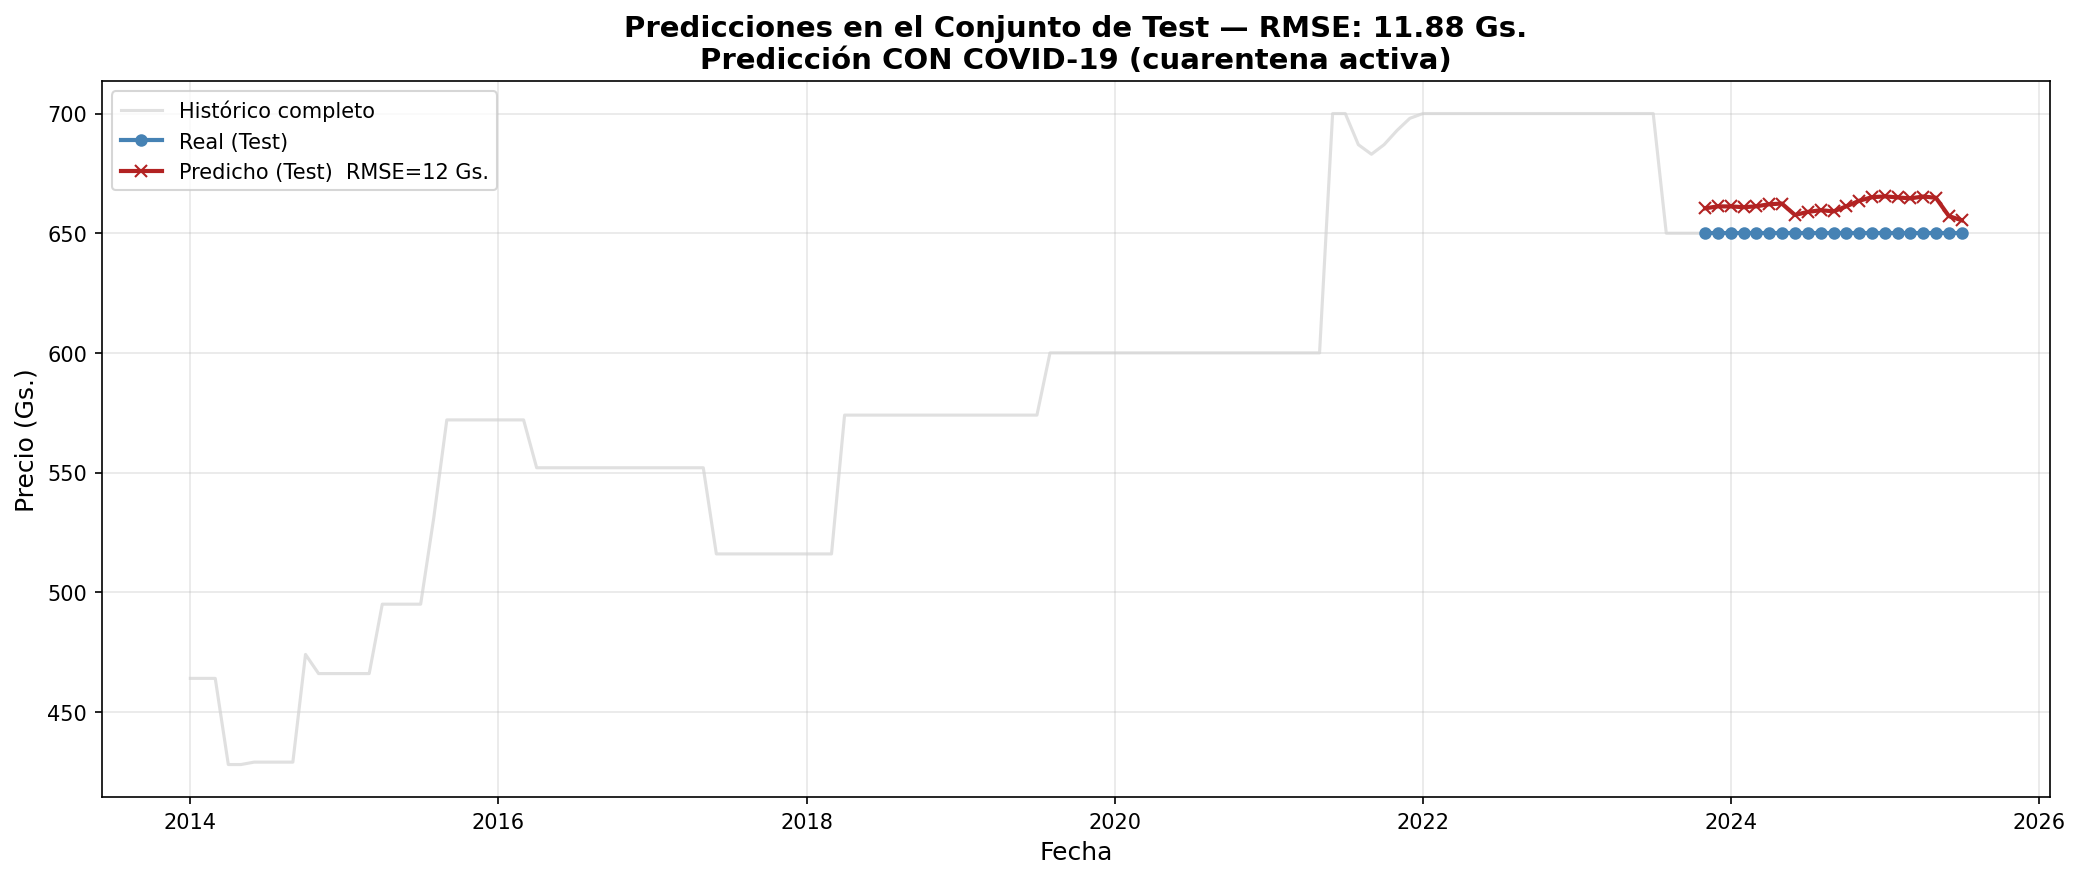
\includegraphics[width=\textwidth]{predicciones/prediccion_ladrillo_gru/resultados_con_covid/final_02_prediccion_test_serie.png}
    \caption{Predicción GRU vs.\ valores reales del precio del ladrillo --- escenario con pandemia, conjunto de prueba.}
    \label{fig:gru_ladrillo_test_cc}
\end{figure}

\begin{figure}[htbp]
    \centering
    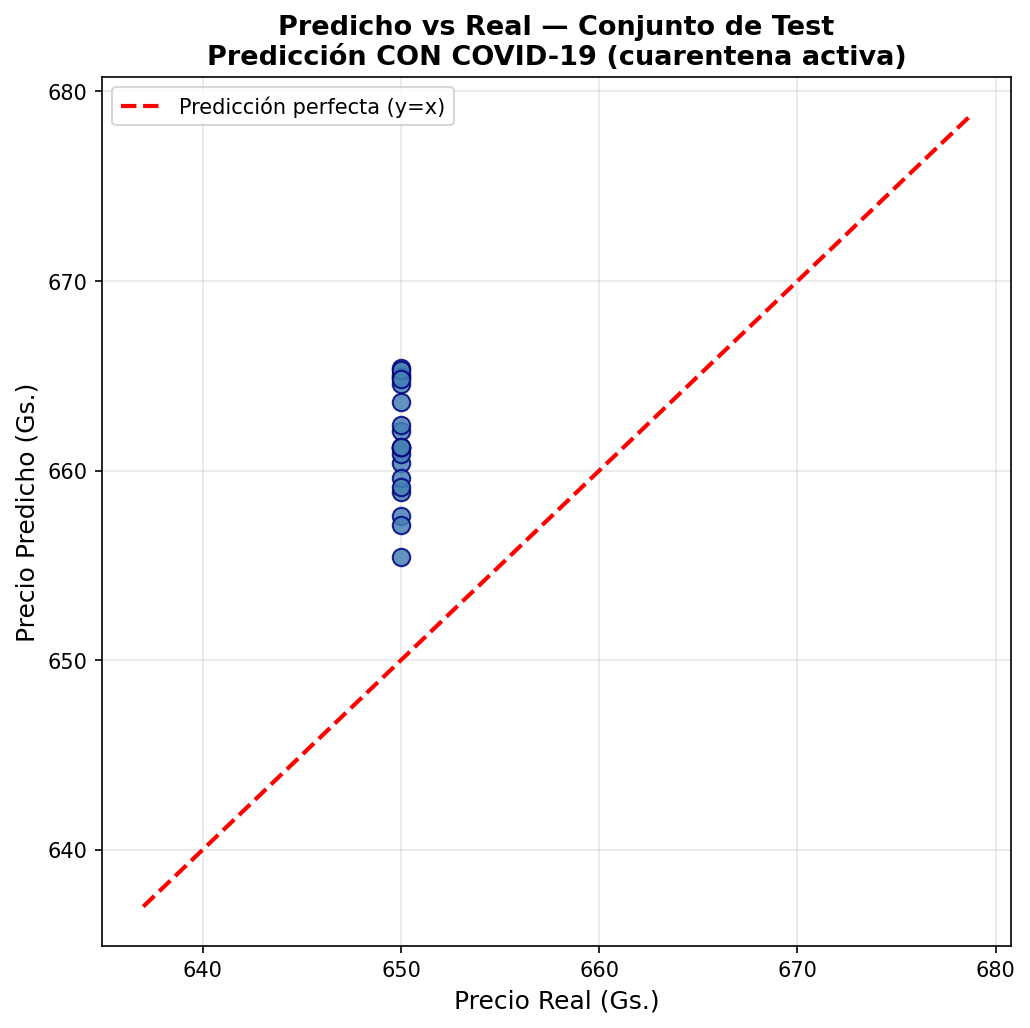
\includegraphics[width=0.8\textwidth]{predicciones/prediccion_ladrillo_gru/resultados_con_covid/final_03_scatter_test.png}
    \caption{Diagrama de dispersión: precio predicho vs.\ real del ladrillo --- escenario con pandemia (GRU).}
    \label{fig:gru_ladrillo_scatter_cc}
\end{figure}

\begin{figure}[htbp]
    \centering
    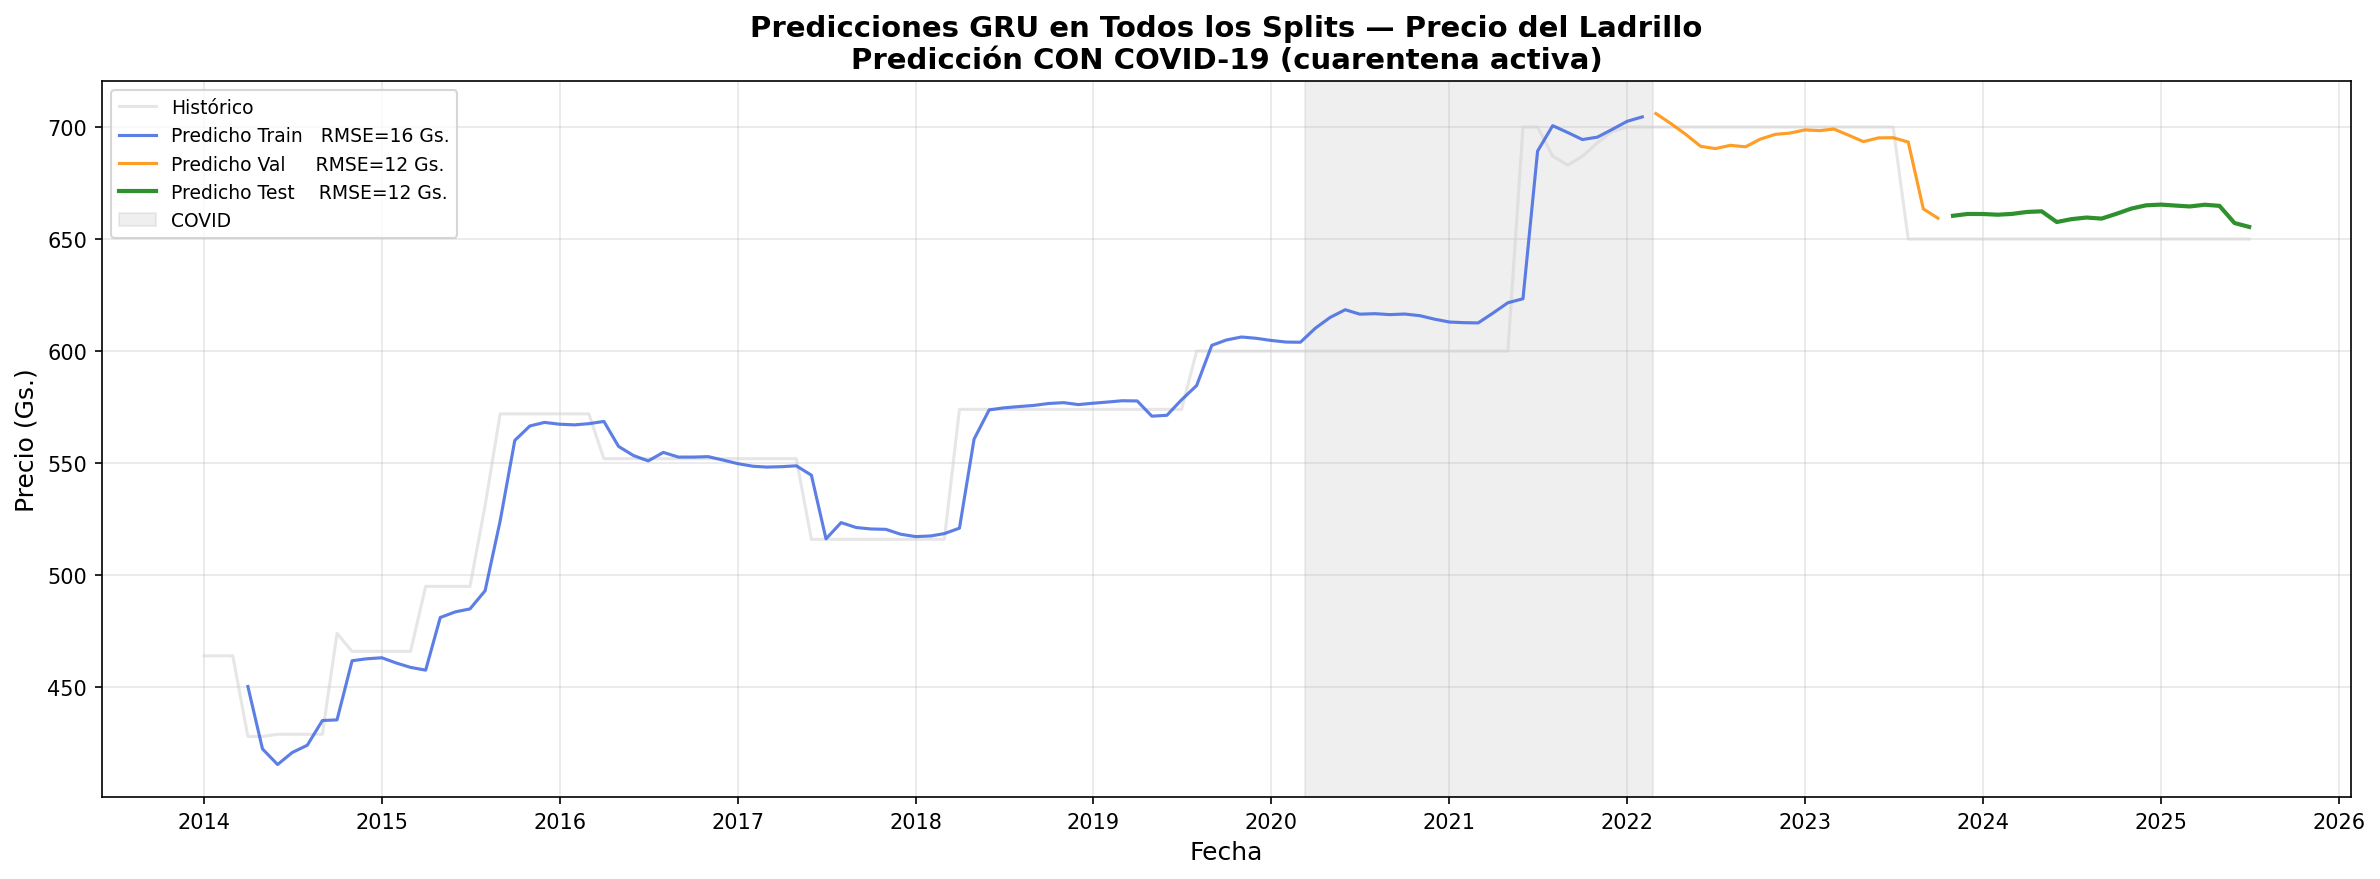
\includegraphics[width=\textwidth]{predicciones/prediccion_ladrillo_gru/resultados_con_covid/final_05_todos_splits.png}
    \caption{Ajuste del modelo GRU del ladrillo sobre las tres particiones --- escenario con pandemia.}
    \label{fig:gru_ladrillo_splits_cc}
\end{figure}

\clearpage
\paragraph{Análisis de Residuos}

\begin{figure}[htbp]
    \centering
    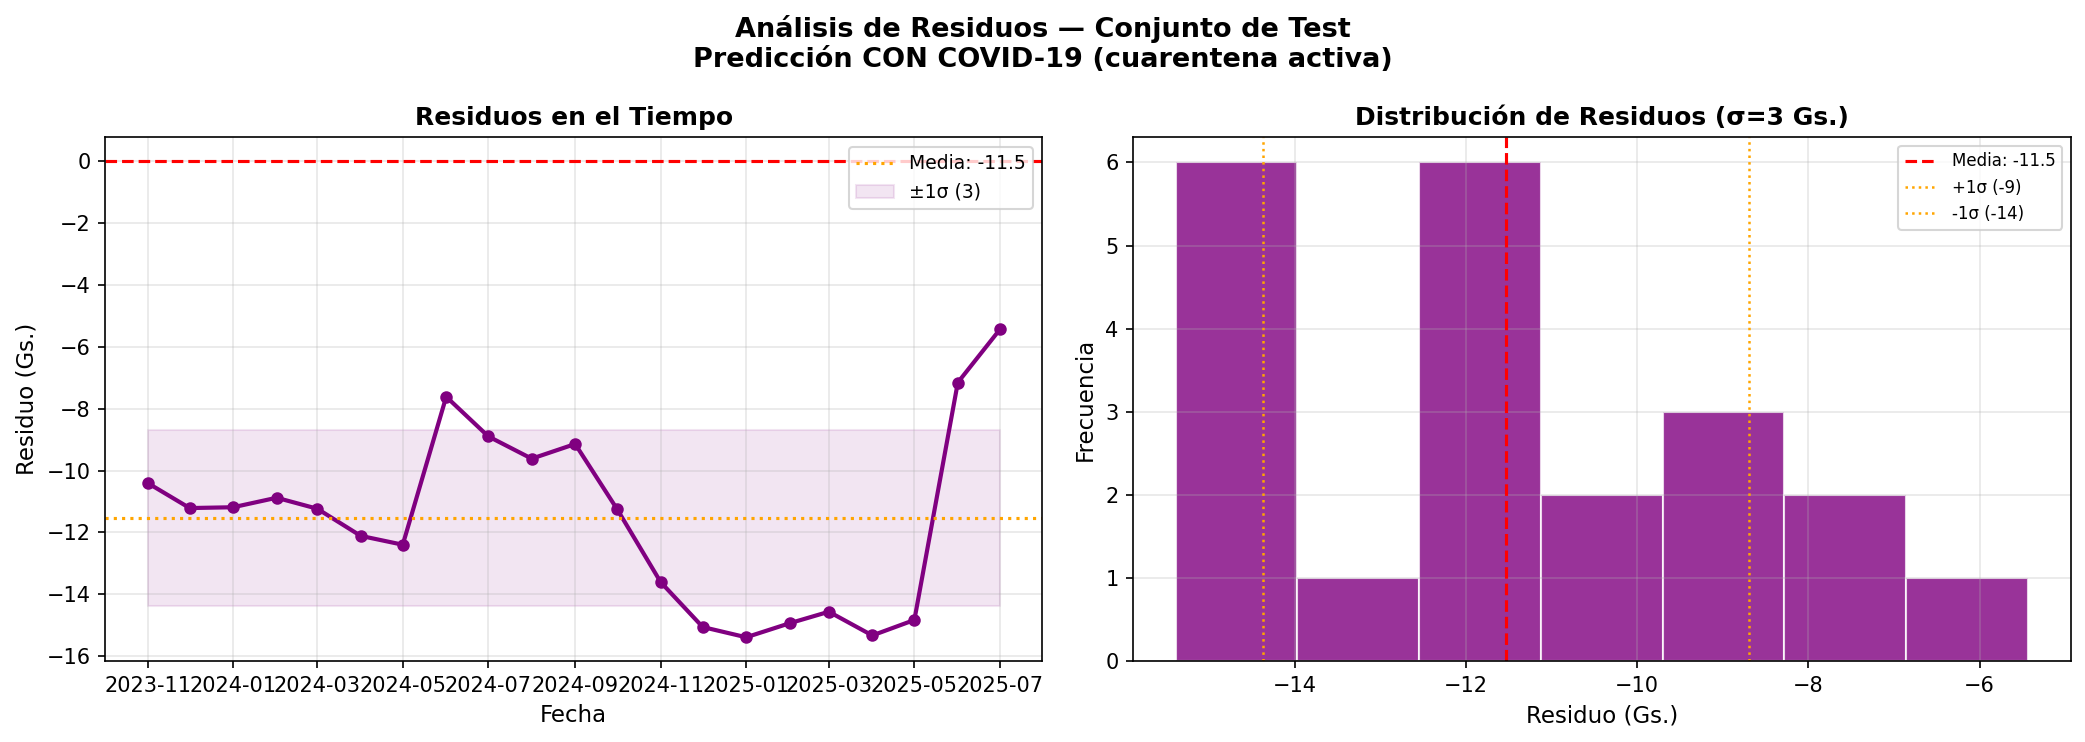
\includegraphics[width=\textwidth]{predicciones/prediccion_ladrillo_gru/resultados_con_covid/final_04_residuos.png}
    \caption{Residuos del modelo GRU para ladrillo --- escenario con pandemia, conjunto de prueba.}
    \label{fig:gru_ladrillo_res_cc}
\end{figure}

\begin{figure}[htbp]
    \centering
    \includegraphics[width=0.8\textwidth]{predicciones/prediccion_ladrillo_gru/resultados_con_covid/residuos_histograma.png}
    \caption{Histograma de residuos del modelo GRU para ladrillo --- escenario con pandemia.}
    \label{fig:gru_ladrillo_reshist_cc}
\end{figure}

\begin{figure}[htbp]
    \centering
    \includegraphics[width=\textwidth]{predicciones/prediccion_ladrillo_gru/resultados_con_covid/residuos_acf_pacf.png}
    \caption{ACF y PACF de los residuos del modelo GRU para ladrillo --- escenario con pandemia.}
    \label{fig:gru_ladrillo_acf_cc}
\end{figure}

\justify
El test de Ljung-Box sobre los residuos del conjunto de prueba muestra un $p$-valor de 0,009 a 10 rezagos (rechaza $H_0$) y de $1{,}13 \times 10^{-9}$ a 20 rezagos (rechaza fuertemente $H_0$). Este resultado indica la presencia de autocorrelación residual significativa en el modelo con pandemia, en contraste con el comportamiento de ruido blanco logrado por el modelo sin pandemia. La mayor autocorrelación residual sugiere que la configuración predeterminada del escenario con pandemia no captura tan eficientemente la estructura temporal de la serie del ladrillo como lo hace el modelo más compacto y propiamente optimizado.

\clearpage
\paragraph{Pronóstico a 24 Meses}

\begin{figure}[htbp]
    \centering
    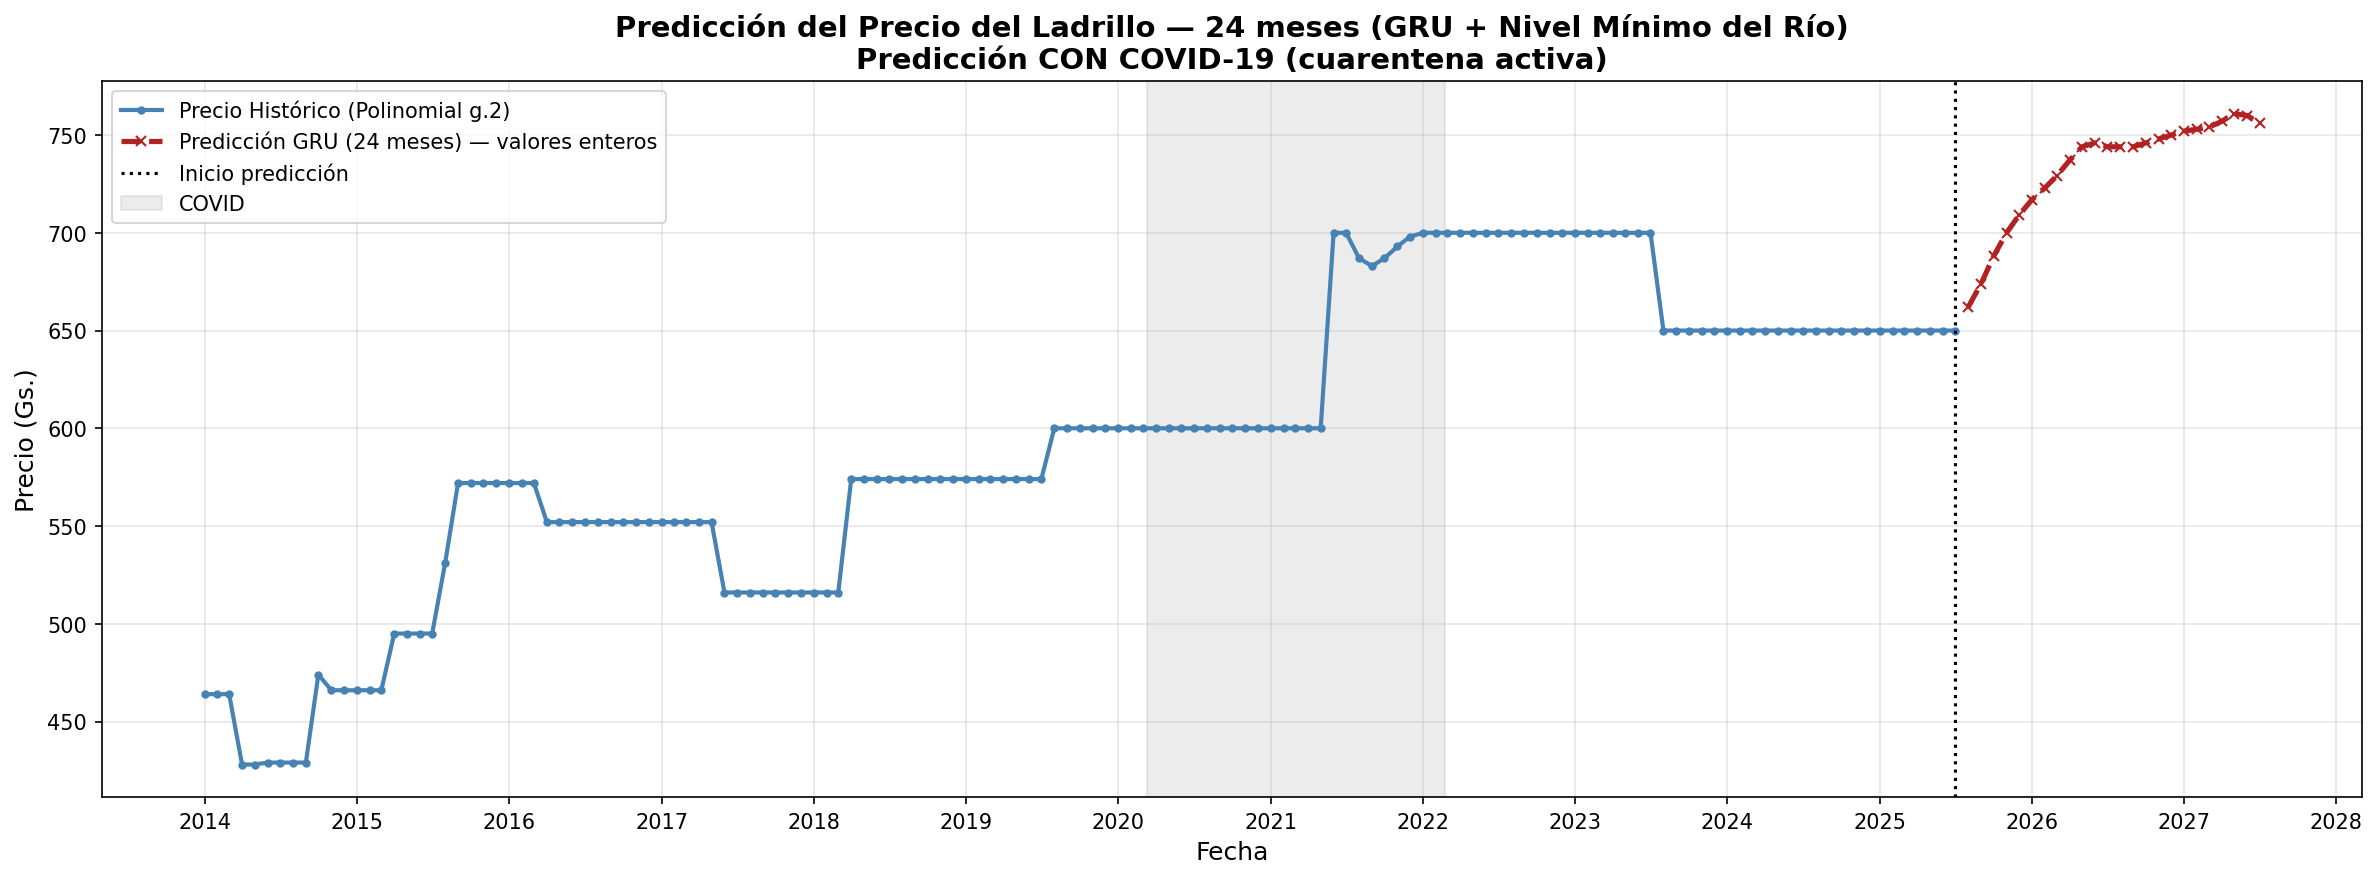
\includegraphics[width=\textwidth]{predicciones/prediccion_ladrillo_gru/resultados_con_covid/final_06_prediccion_futura_completa.png}
    \caption{Pronóstico GRU del precio del ladrillo a 24 meses --- escenario con pandemia: serie histórica y proyección.}
    \label{fig:gru_ladrillo_pred_con_covid}
\end{figure}

\begin{figure}[htbp]
    \centering
    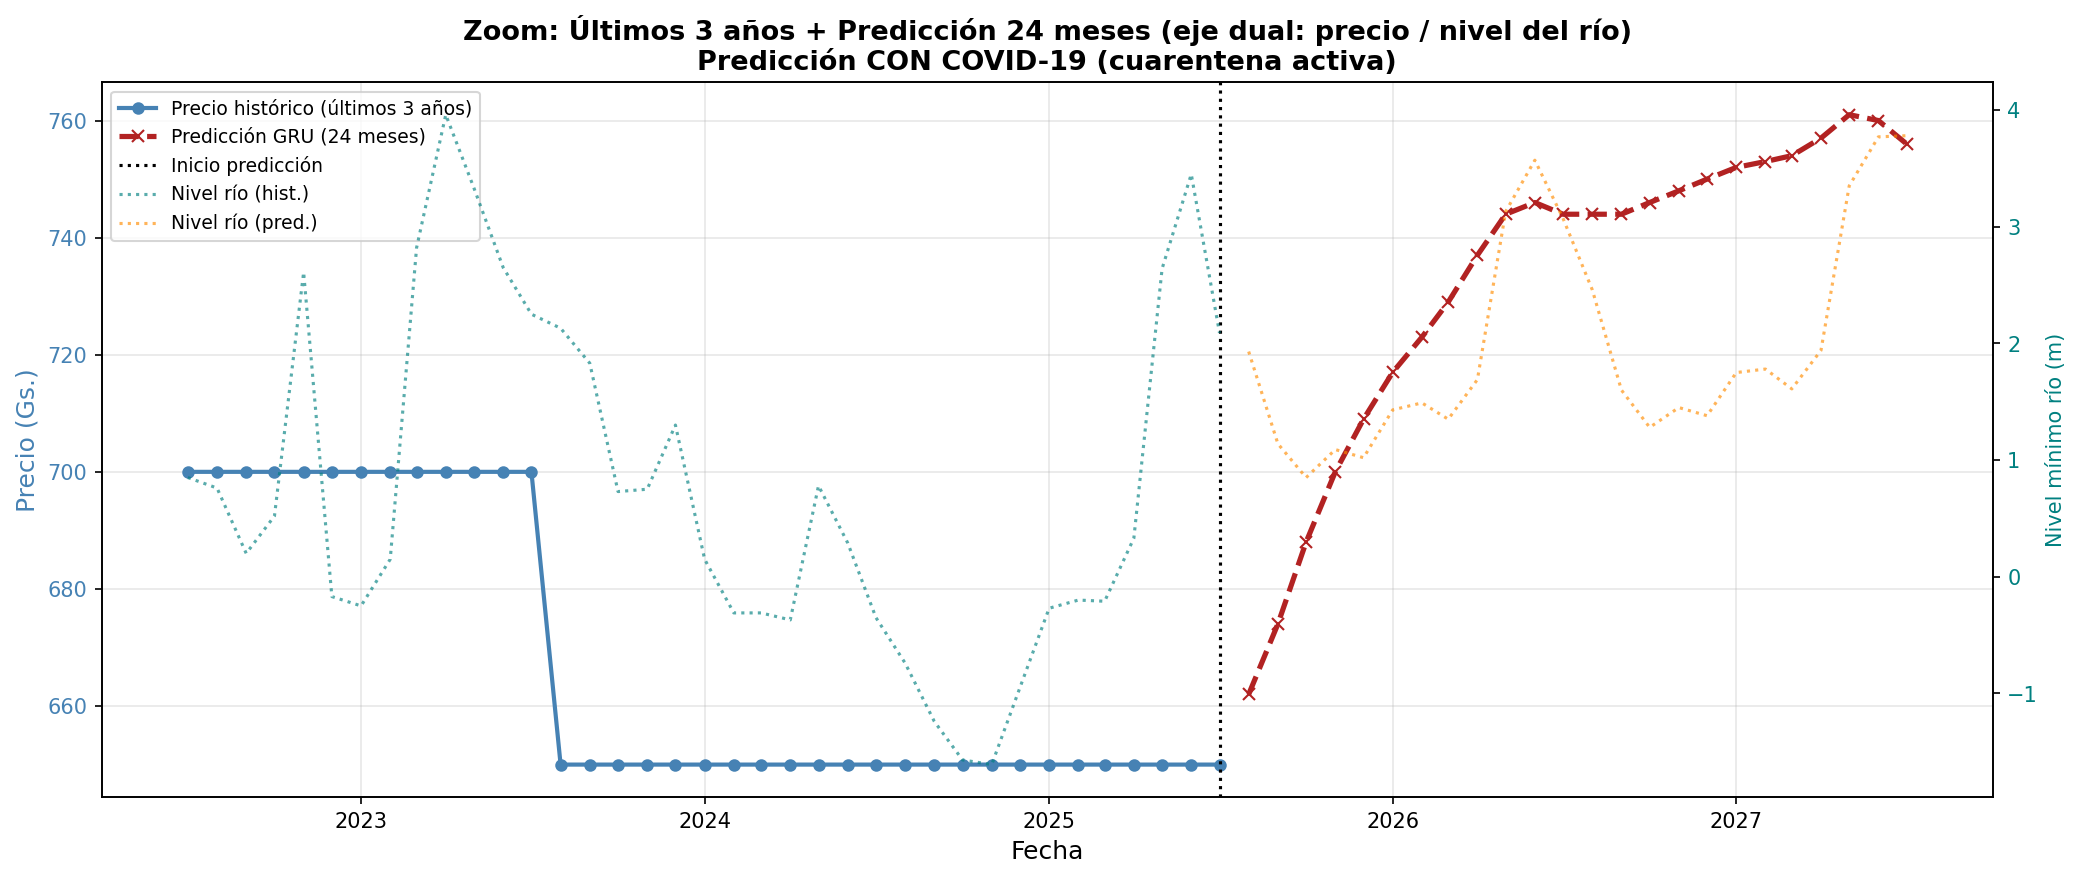
\includegraphics[width=\textwidth]{predicciones/prediccion_ladrillo_gru/resultados_con_covid/final_07_prediccion_zoom_dual.png}
    \caption{Zoom sobre la transición entre datos observados y pronóstico GRU del ladrillo --- escenario con pandemia.}
    \label{fig:gru_ladrillo_zoom_con_covid}
\end{figure}

\begin{figure}[htbp]
    \centering
    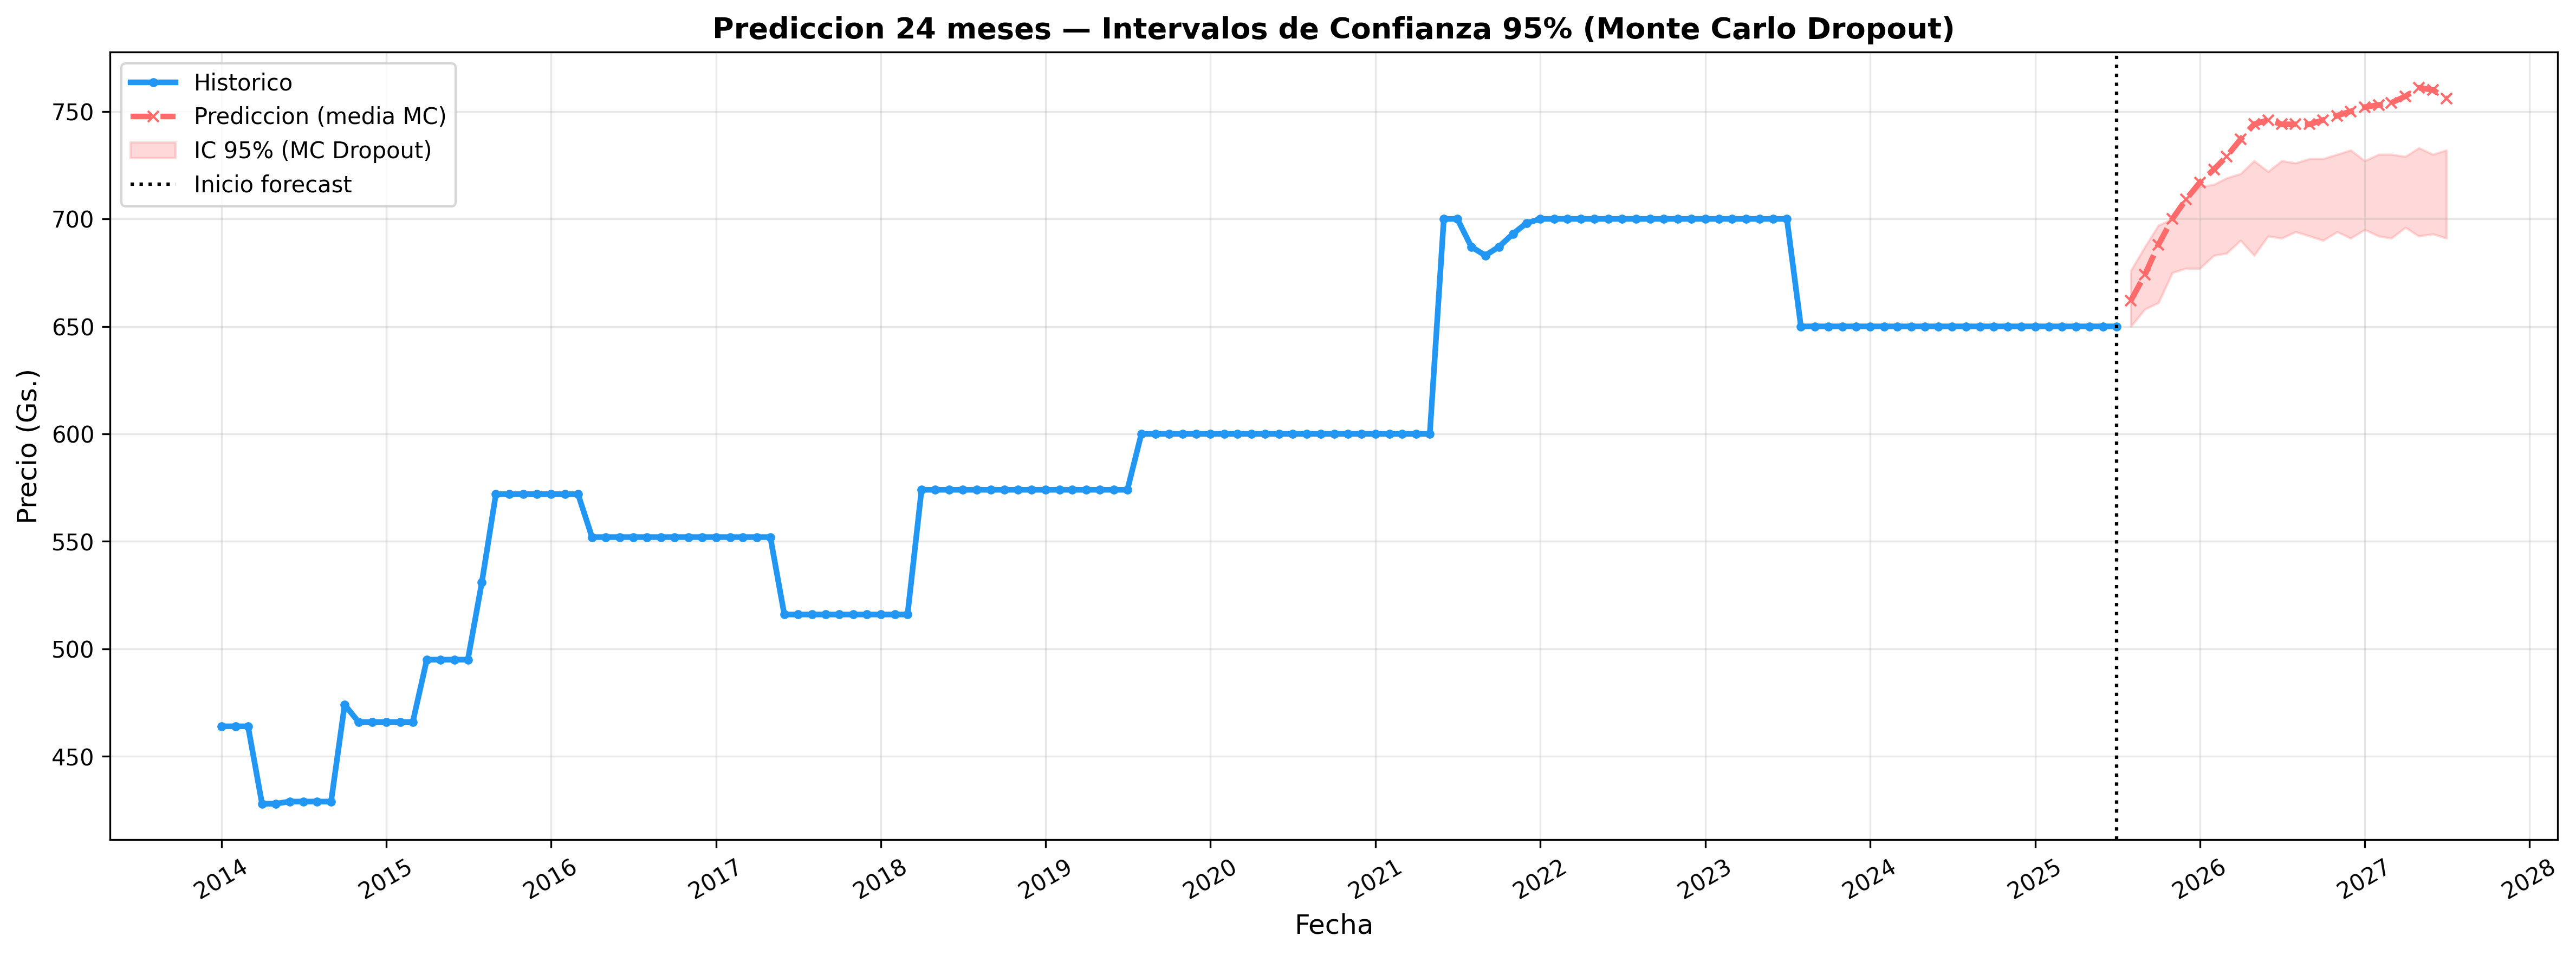
\includegraphics[width=\textwidth]{predicciones/prediccion_ladrillo_gru/resultados_con_covid/forecast_ic_monte_carlo.png}
    \caption{IC Monte Carlo Dropout del pronóstico GRU para ladrillo --- escenario con pandemia.}
    \label{fig:gru_ladrillo_ic_con_covid}
\end{figure}

\justify
Bajo el escenario con efecto pandémico, el rango de precios proyectado para el ladrillo se sitúa entre Gs.~662 y Gs.~761. El límite superior es ligeramente mayor que en el escenario sin pandemia (Gs.~726), lo que indica que el modelo captura un efecto alcista acumulado de la variable pandémica sobre el precio del ladrillo hacia el final del horizonte de predicción.

\justify
La divergencia en la interpretación del efecto pandémico entre los modelos GRU del cemento y del ladrillo es uno de los hallazgos más relevantes del estudio. Para el cemento, la GRU asoció la pandemia con una contracción de precios (rango Gs.~46.048--53.874 con pandemia versus Gs.~55.600--61.845 sin pandemia); para el ladrillo, el modelo capturó un efecto alcista moderado (Gs.~662--761 con pandemia versus Gs.~662--726 sin pandemia). Para el cemento, la pandemia fue interpretada como un factor de contracción de la demanda; para el ladrillo, como un leve impulso ascendente, lo que es más consistente con la evolución observada de los precios durante 2020--2022.
